\section{Phụ lục}
\subsection{Thiết kế giao diện hệ thống}
\subsubsection{Thiết kế giao diện cho khách hàng}

\subsubsubsection {Trang chủ}
\begin{figure}[H]
    \centering
    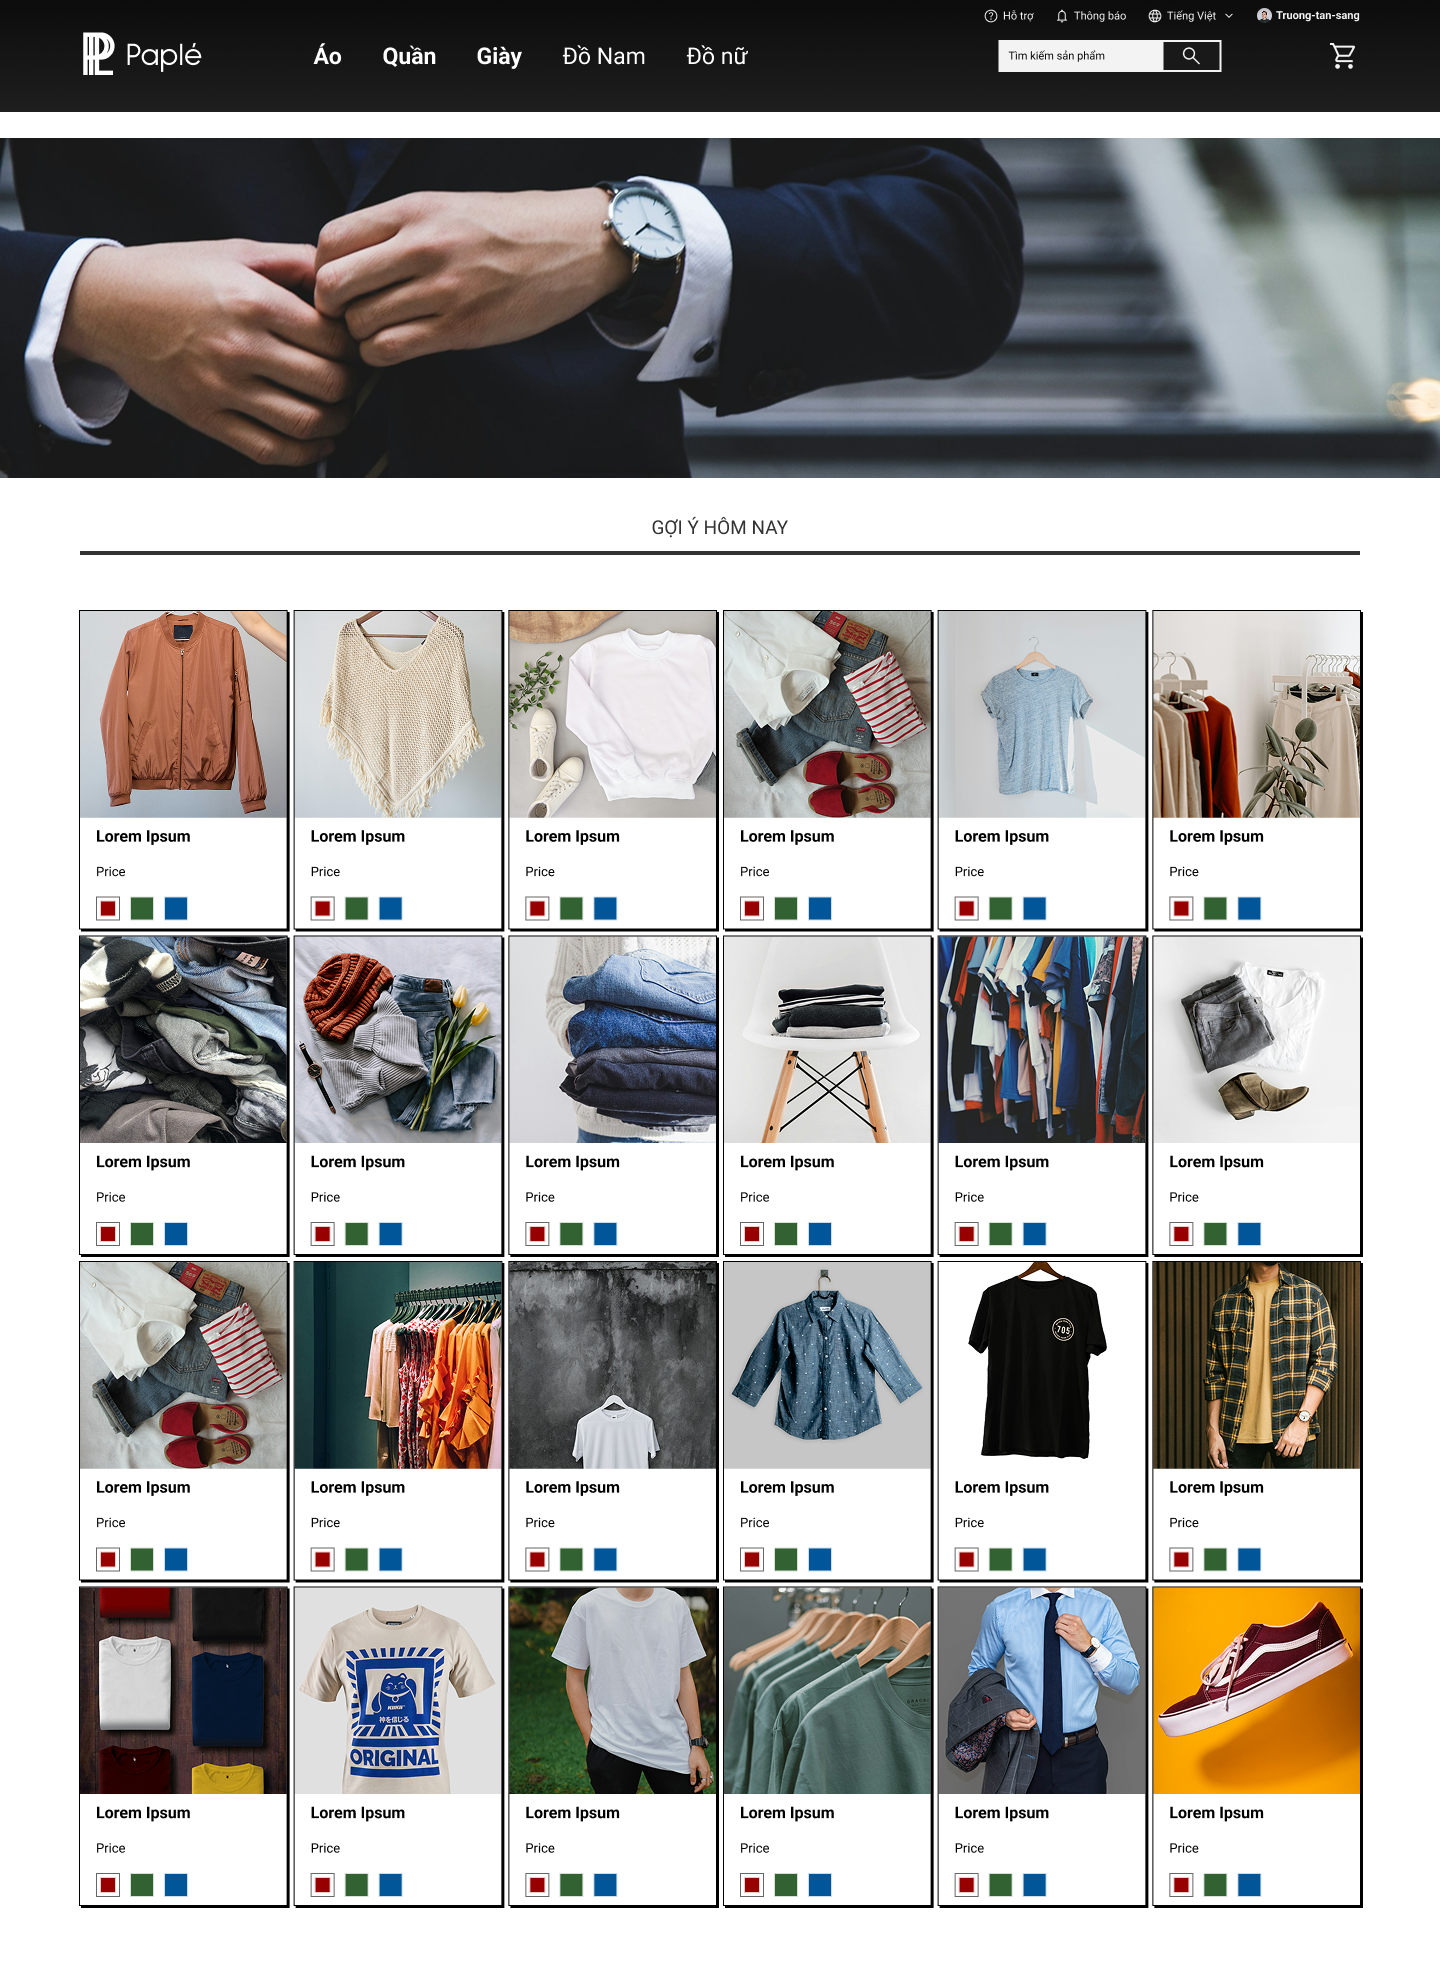
\includegraphics[width=1\textwidth]{Images/MockUp/Customer/Home.png}
    \vspace{0.5cm}
    \caption{Giao diện trang chủ}
    \label{fig: Giao diện trang chủ}
\end{figure}
\noindent\textbf{Các thao tác chính:} Người dùng có thể duyệt các sản phẩm nổi bật, xem danh mục sản phẩm, tìm kiếm sản phẩm qua thanh tìm kiếm, xem giỏ hàng, quản lý tài khoản, và truy cập chức năng chat hỗ trợ khách hàng.
\subsubsubsection {Xem Sản phẩm theo Loại/Tìm kiếm Sản phẩm}
\begin{figure}[H]
    \centering
    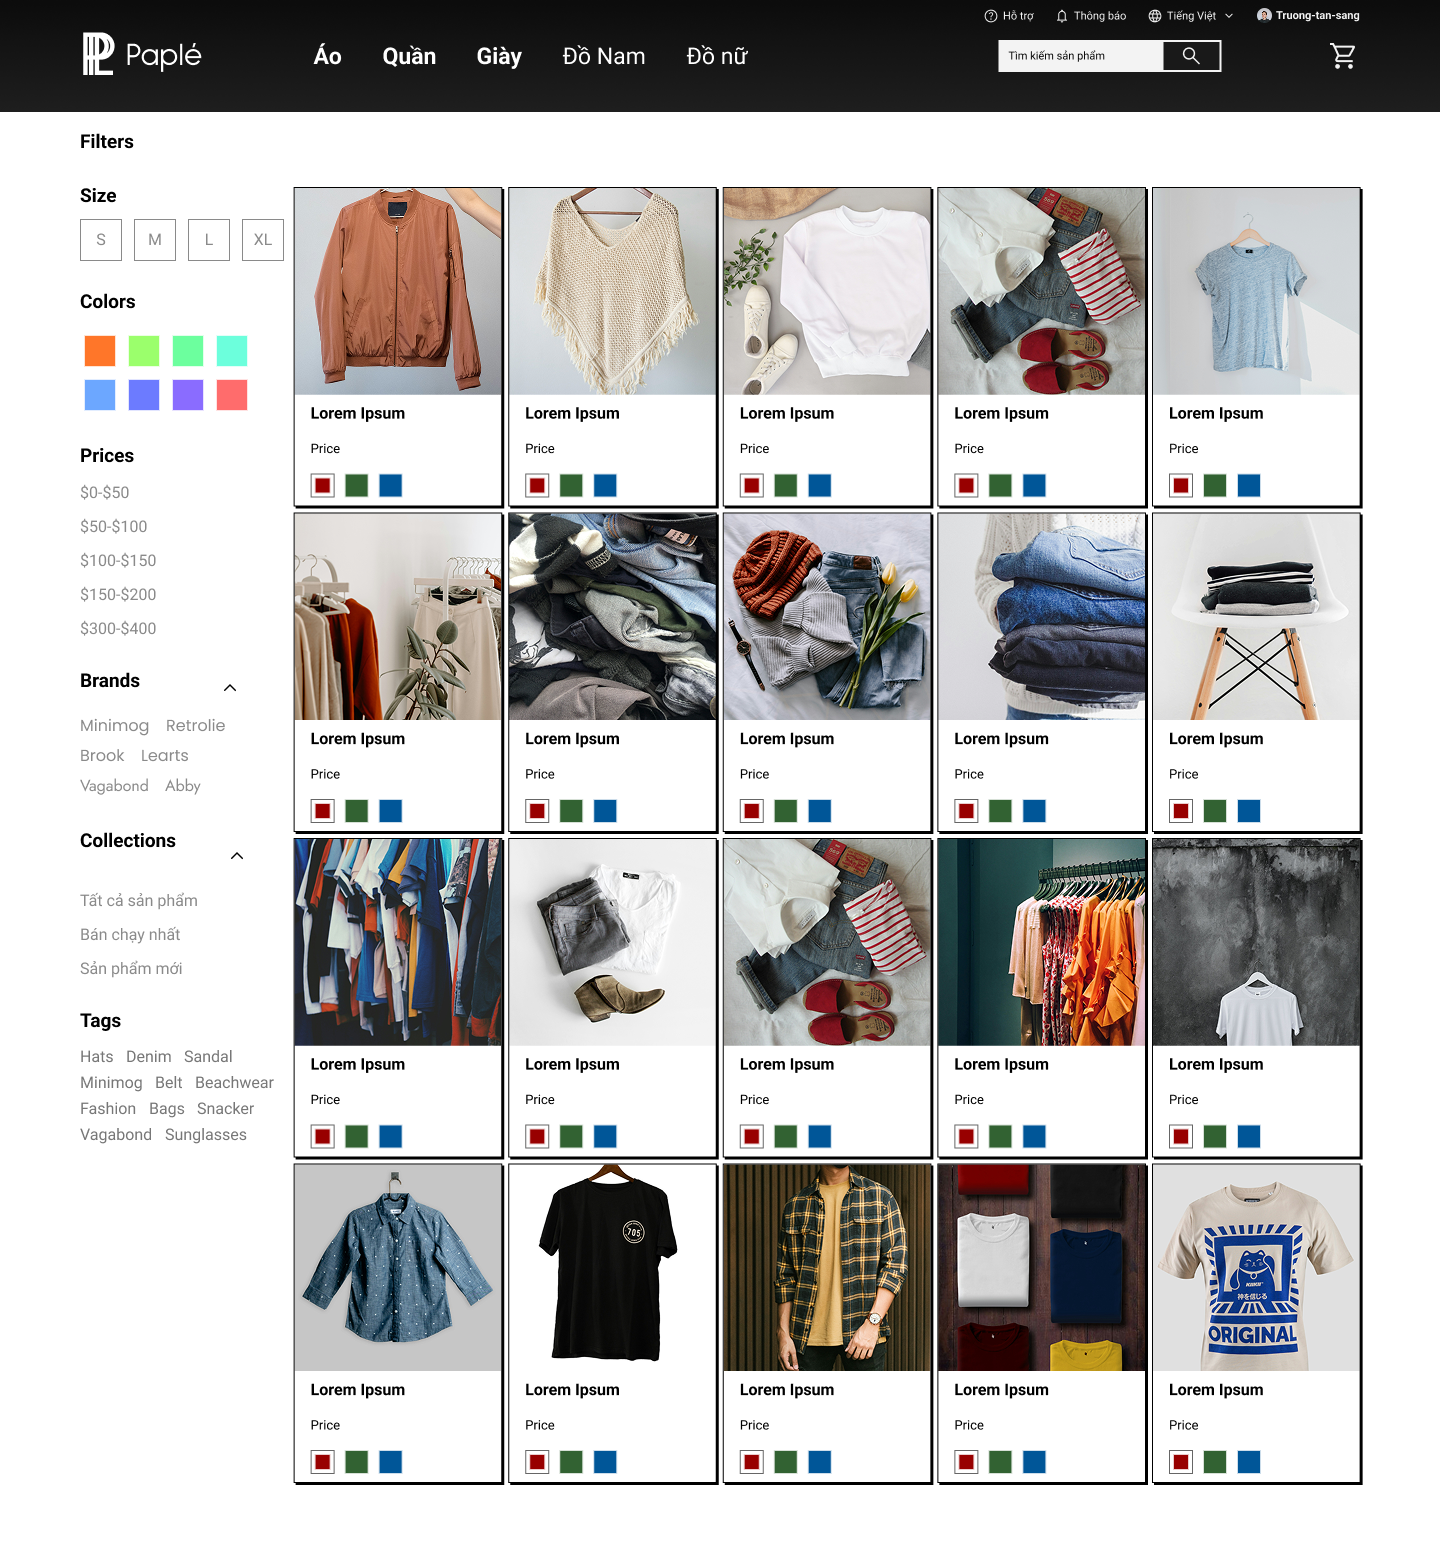
\includegraphics[width=1\textwidth]{Images/MockUp/Customer/Categories+Search.png}
    \vspace{0.5cm}
    \caption{Giao diện Xem theo loại/Tìm kiếm}
    \label{fig: Giao diện Xem theo loại/Tìm kiếm}
\end{figure}
\noindent\textbf{Các thao tác chính:} Người dùng có thể lọc sản phẩm theo danh mục, sắp xếp theo giá hoặc đánh giá, tìm kiếm theo từ khóa, xem chi tiết sản phẩm, thêm sản phẩm vào giỏ hàng, và so sánh các sản phẩm khác nhau.

\subsubsubsection {Tính năng Chăm sóc khách hàng}
\begin{enumerate}
    \item Màn hình người dùng:
          \begin{figure}[H]
              \centering
              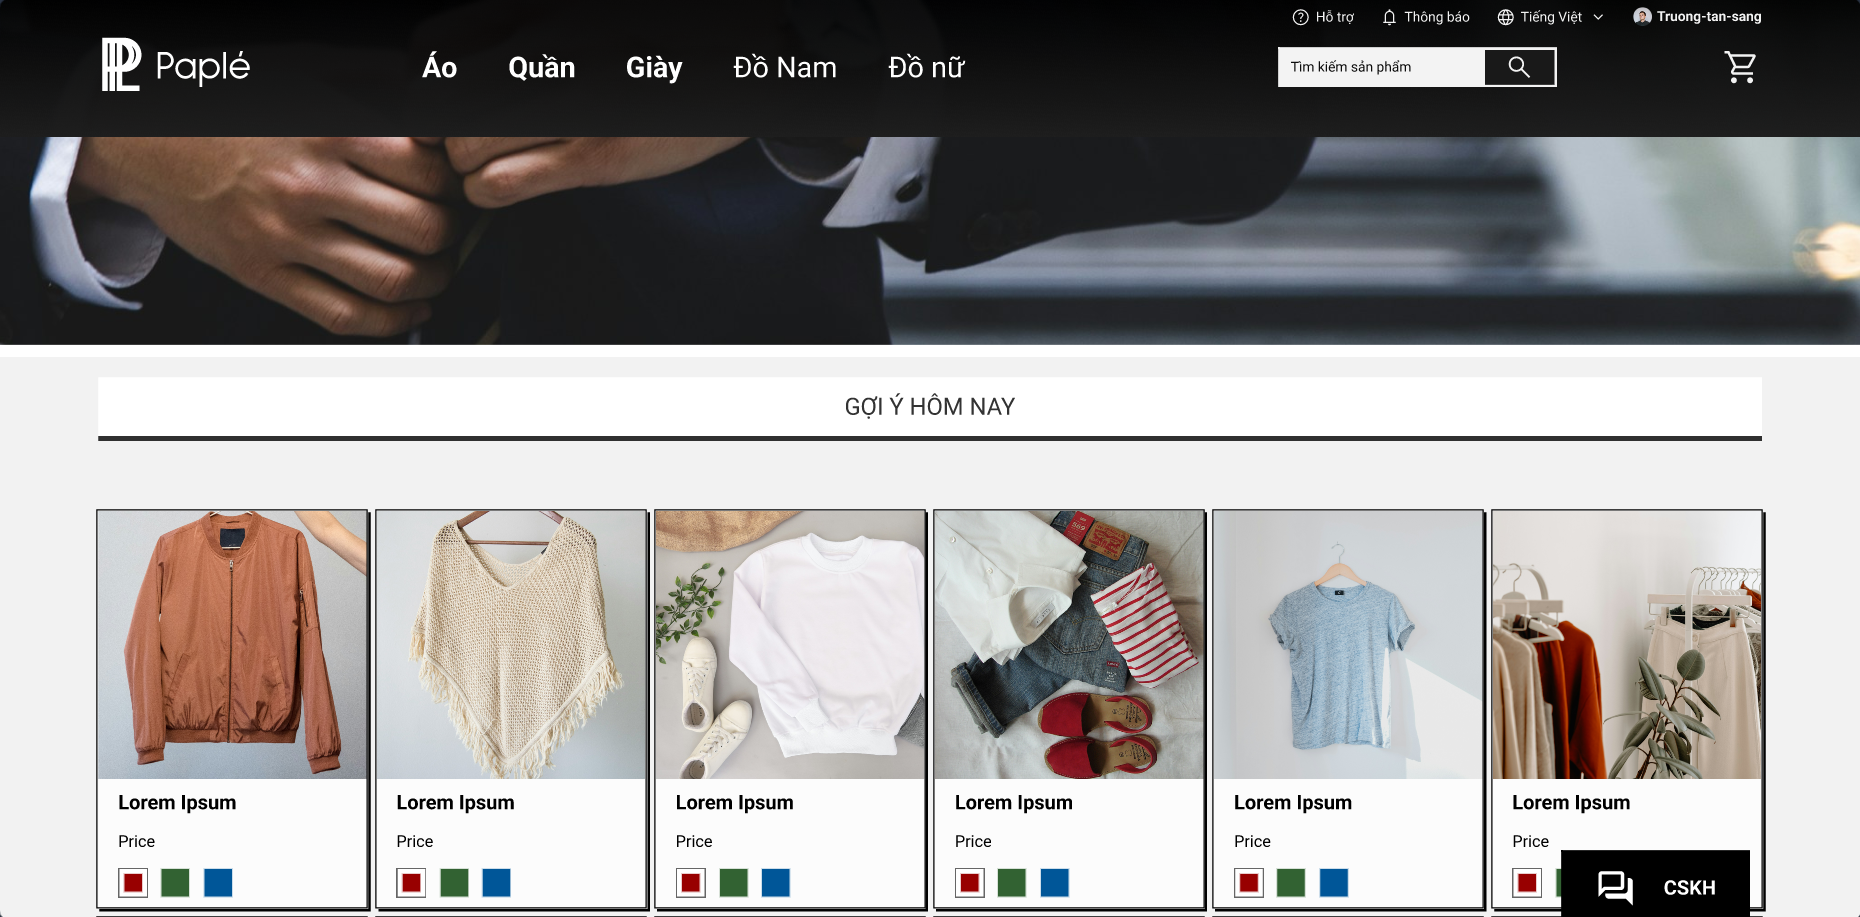
\includegraphics[width=1\textwidth]{Images/MockUp/Customer/Home-View.png}
              \vspace{0.5cm}
              \caption{Giao diện trang chủ (view)}
              \label{fig: Màn hình người dùng}
          \end{figure}
          \noindent\textbf{Các thao tác chính:} Nút chăm sóc khách hàng có thể expand ra để mở khung chat với nhân viên cửa hàng để nhận hỗ trợ.
    \item Màn hình người dùng (sau khi expand tính năng Chat):
          \begin{figure}[H]
              \centering
              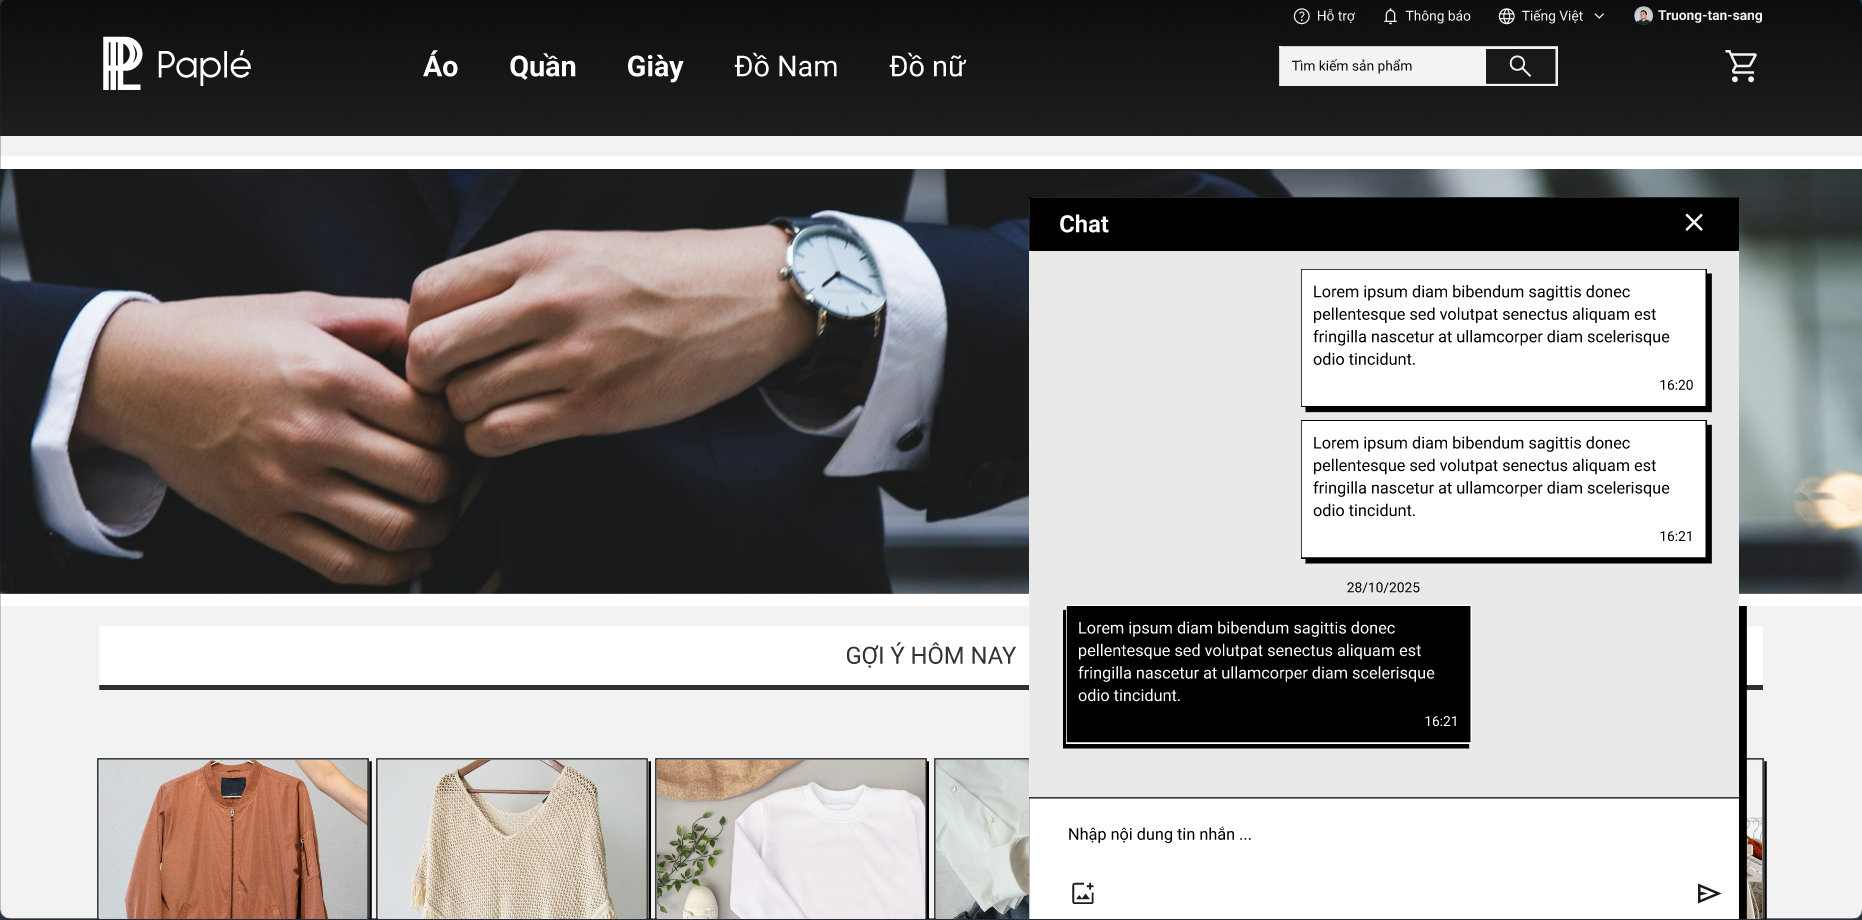
\includegraphics[width=1\textwidth]{Images/MockUp/Customer/Home-Message.png}
              \vspace{0.5cm}
              \caption{Giao diện trang chủ (message)}
              \label{fig: Màn hình người dùng sau khi expand tính năng Chat}
          \end{figure}
          \noindent\textbf{Các thao tác chính:} Gửi và nhận tin nhắn với nhân viên hỗ trợ, xem lịch sử cuộc trò chuyện, gửi hình ảnh, và đóng cửa sổ chat.
\end{enumerate}
\subsubsubsection {Giỏ hàng}
\begin{figure}[H]
    \centering
    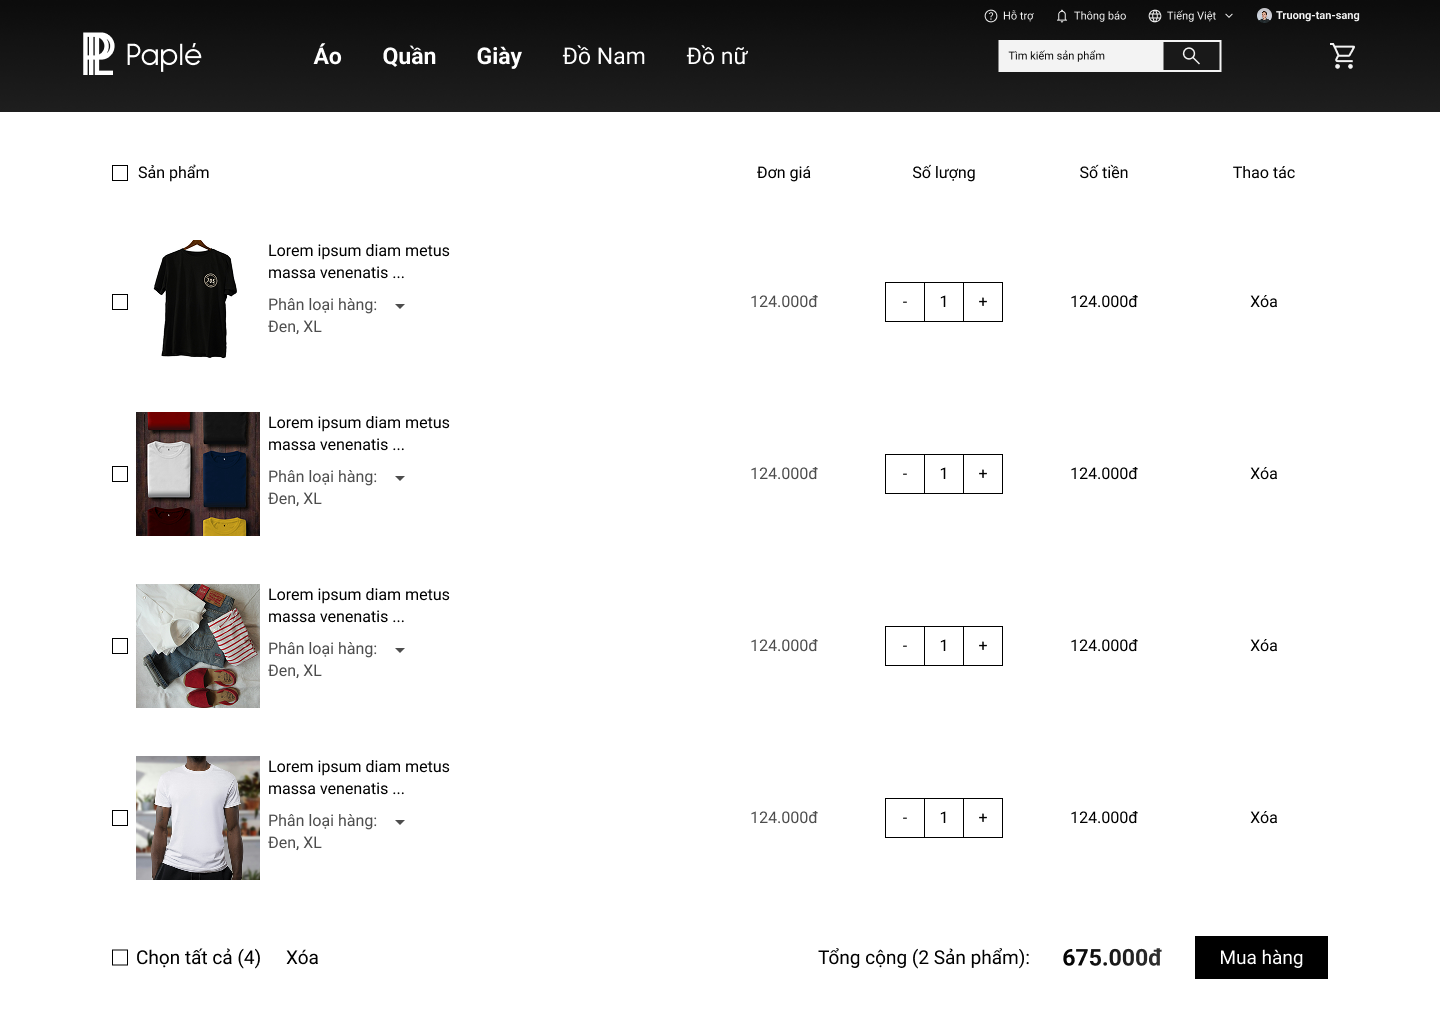
\includegraphics[width=1\textwidth]{Images/MockUp/Customer/Cart.png}
    \vspace{0.5cm}
    \caption{Giao diện Giỏ hàng}
    \label{fig: Giao diện Giỏ hàng}
\end{figure}
\noindent\textbf{Các thao tác chính:} Xem danh sách sản phẩm trong giỏ, thay đổi số lượng sản phẩm, xóa sản phẩm, xem tổng tiền và tiến hành thanh toán.
\subsubsubsection {Thanh toán}
\begin{figure}[H]
    \centering
    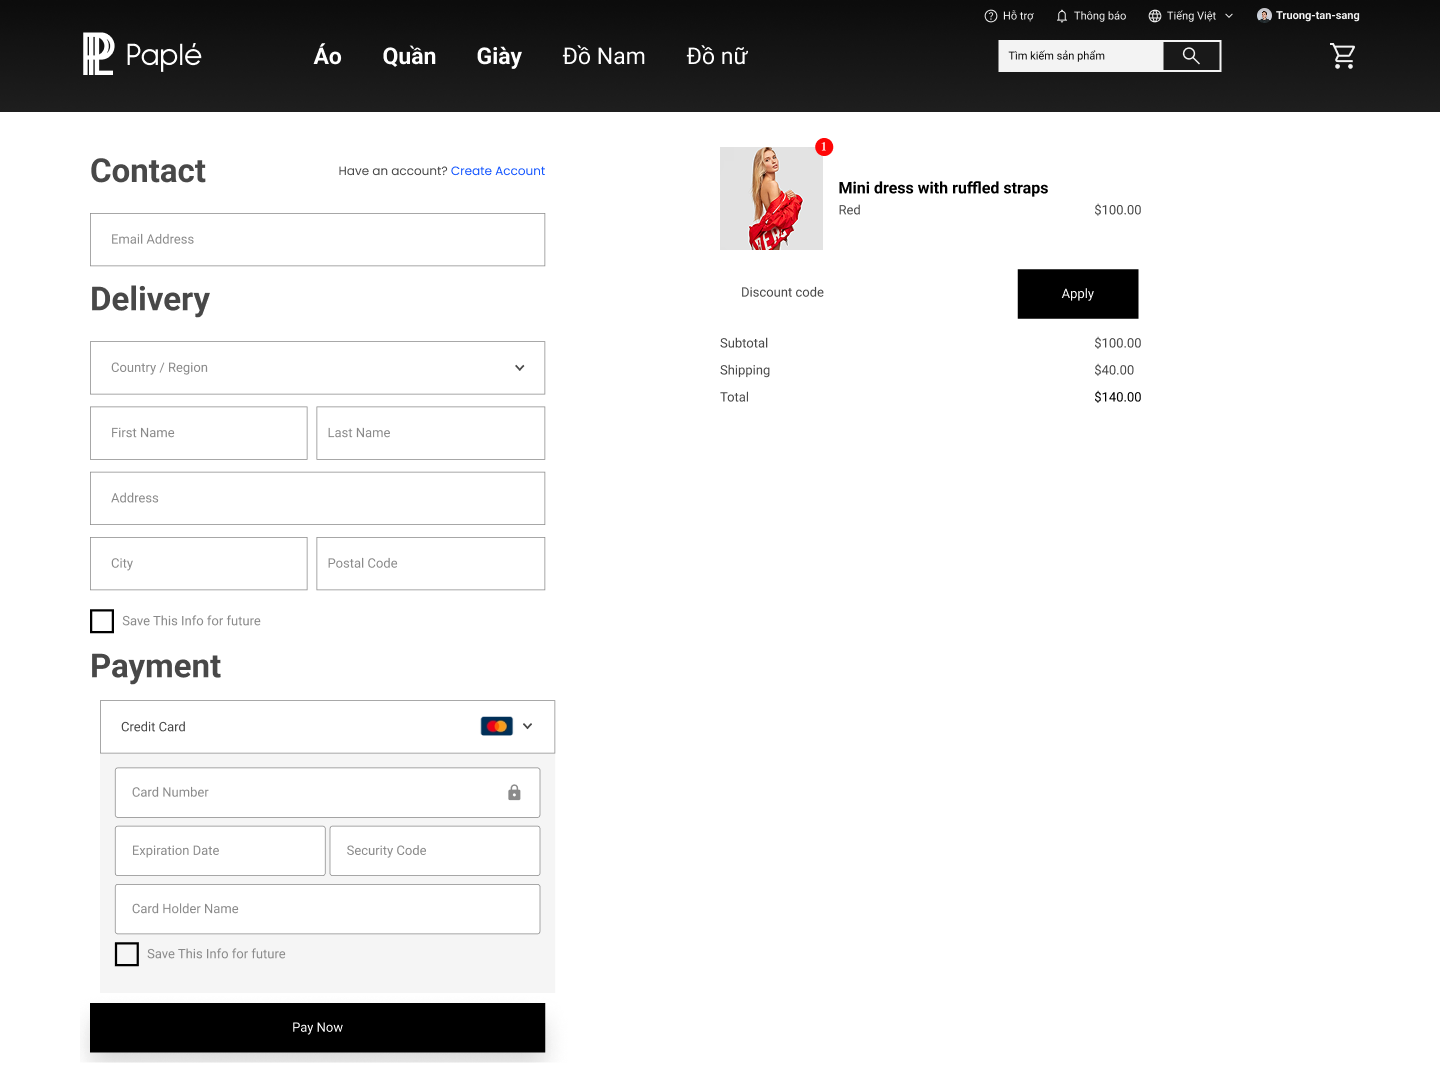
\includegraphics[width=1\textwidth]{Images/MockUp/Customer/Checkout.png}
    \vspace{0.5cm}
    \caption{Giao diện Thanh toán}
    \label{fig: Giao diện Thanh toán}
\end{figure}
\noindent\textbf{Các thao tác chính:} Nhập/chọn địa chỉ giao hàng, chọn phương thức thanh toán, xem chi tiết đơn hàng, nhập mã voucher, xác nhận đơn hàng và hoàn tất giao dịch.
\subsubsubsection {Chi tiết sản phẩm}
\begin{figure}[H]
    \centering
    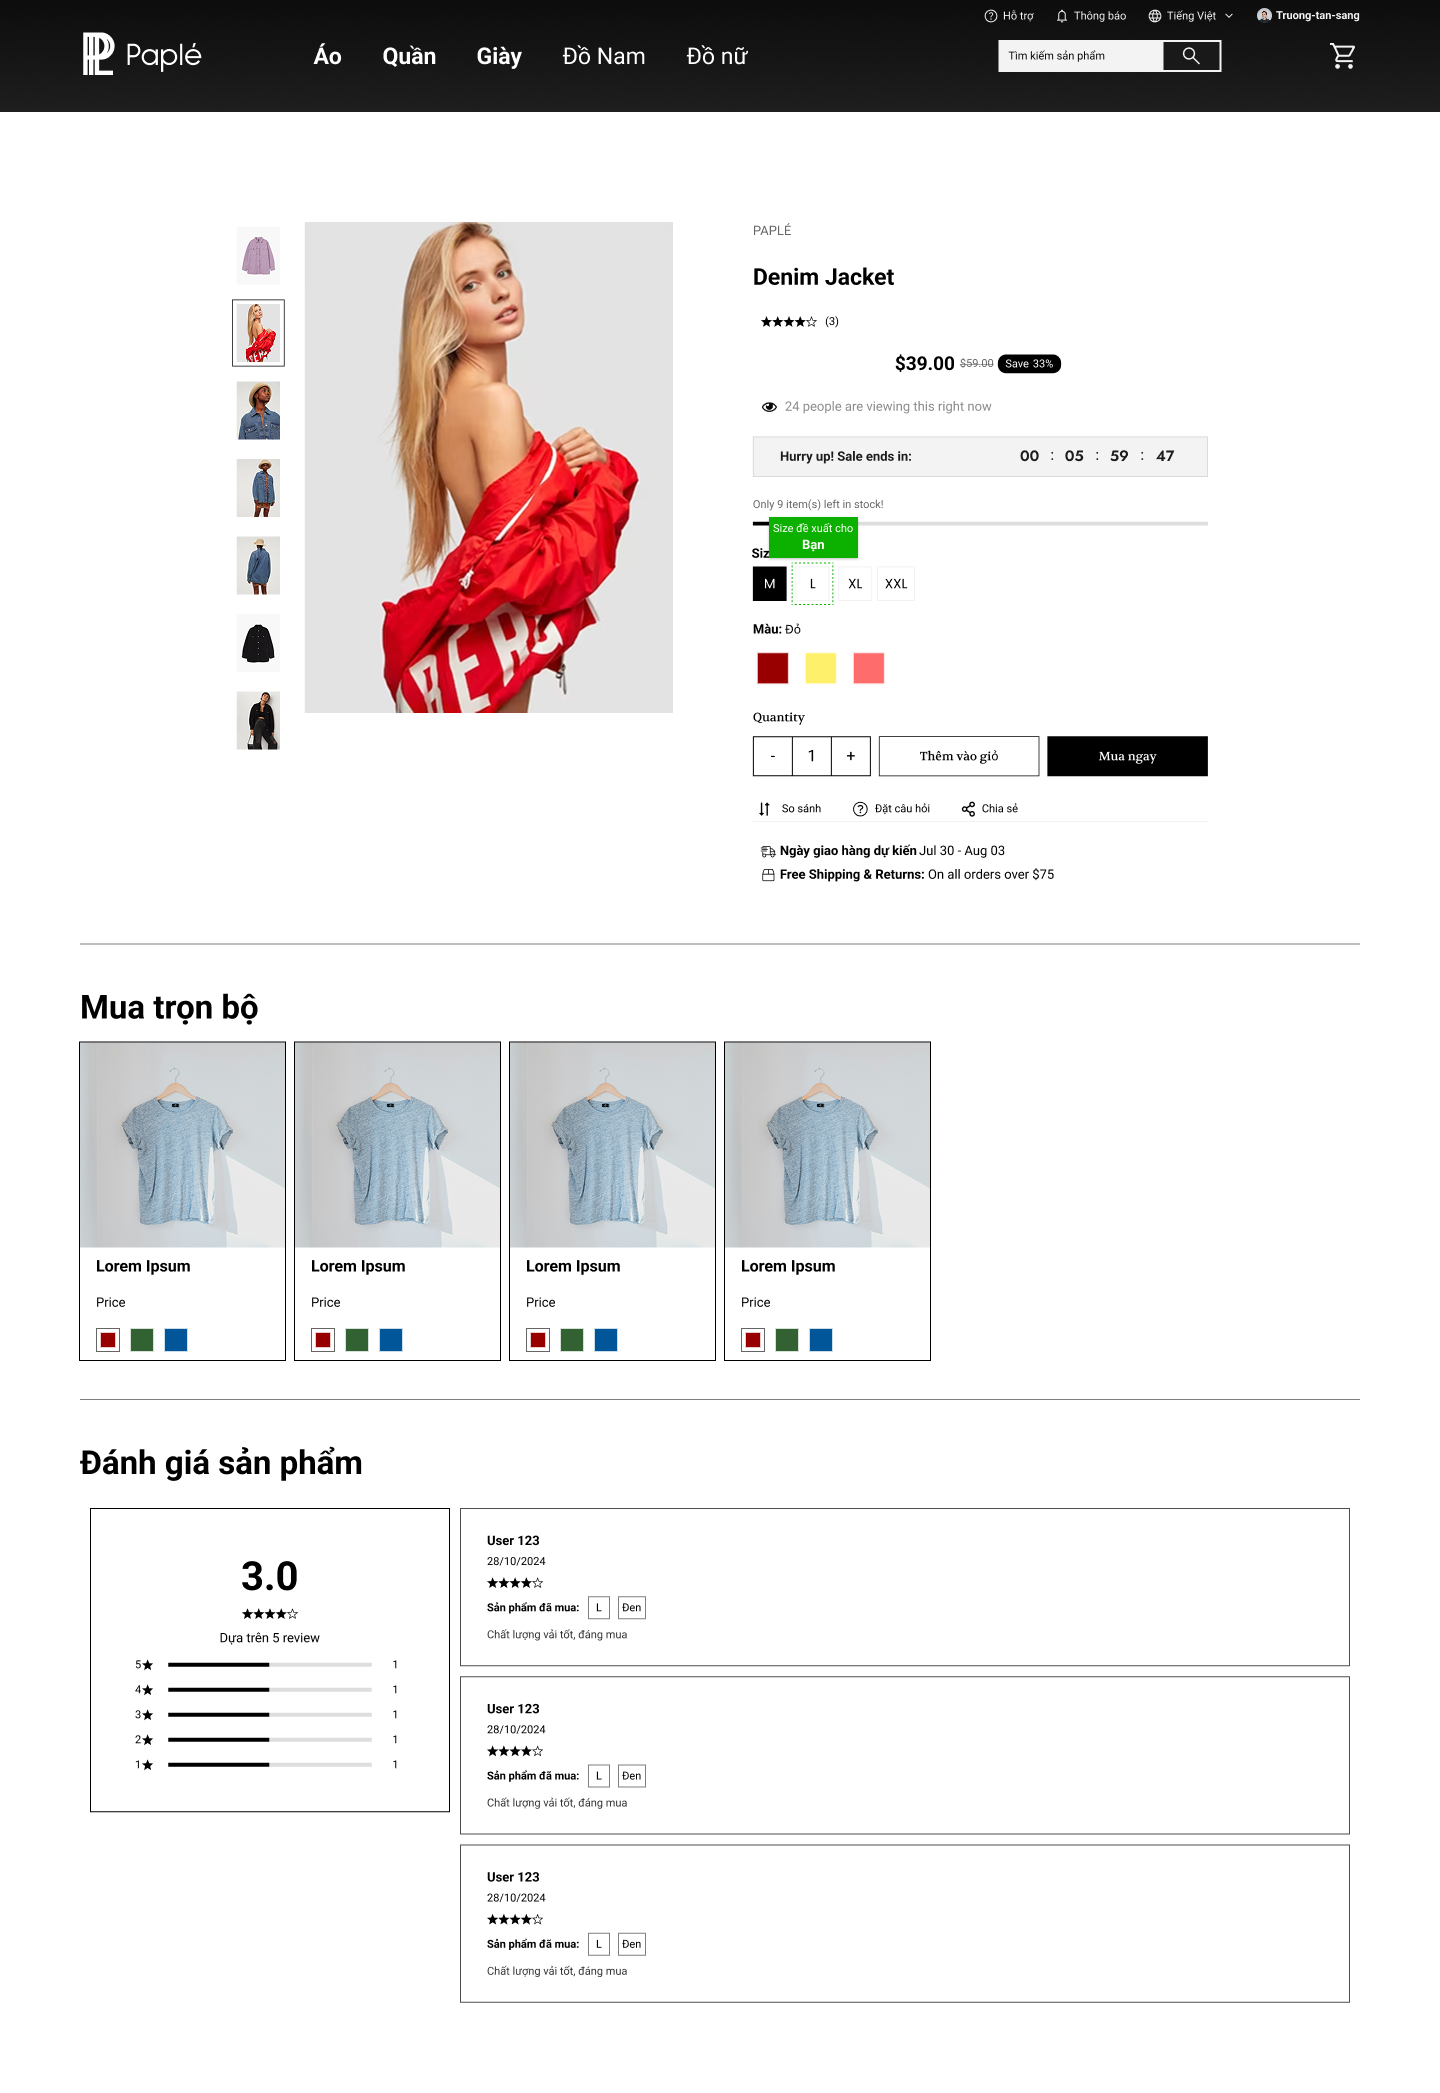
\includegraphics[width=1\textwidth]{Images/MockUp/Customer/Product.png}
    \vspace{0.5cm}
    \caption{Giao diện Chi tiết sản phẩm}
    \label{fig: Giao diện Chi tiết sản phẩm}
\end{figure}
\noindent\textbf{Các thao tác chính:} Xem hình ảnh sản phẩm chi tiết, chọn kích cỡ và màu sắc, xem thông tin mô tả, giá cả và đánh giá, thêm vào giỏ hàng, mua ngay.
\subsubsubsection {So sánh Sản phẩm}
\begin{figure}[H]
    \centering
    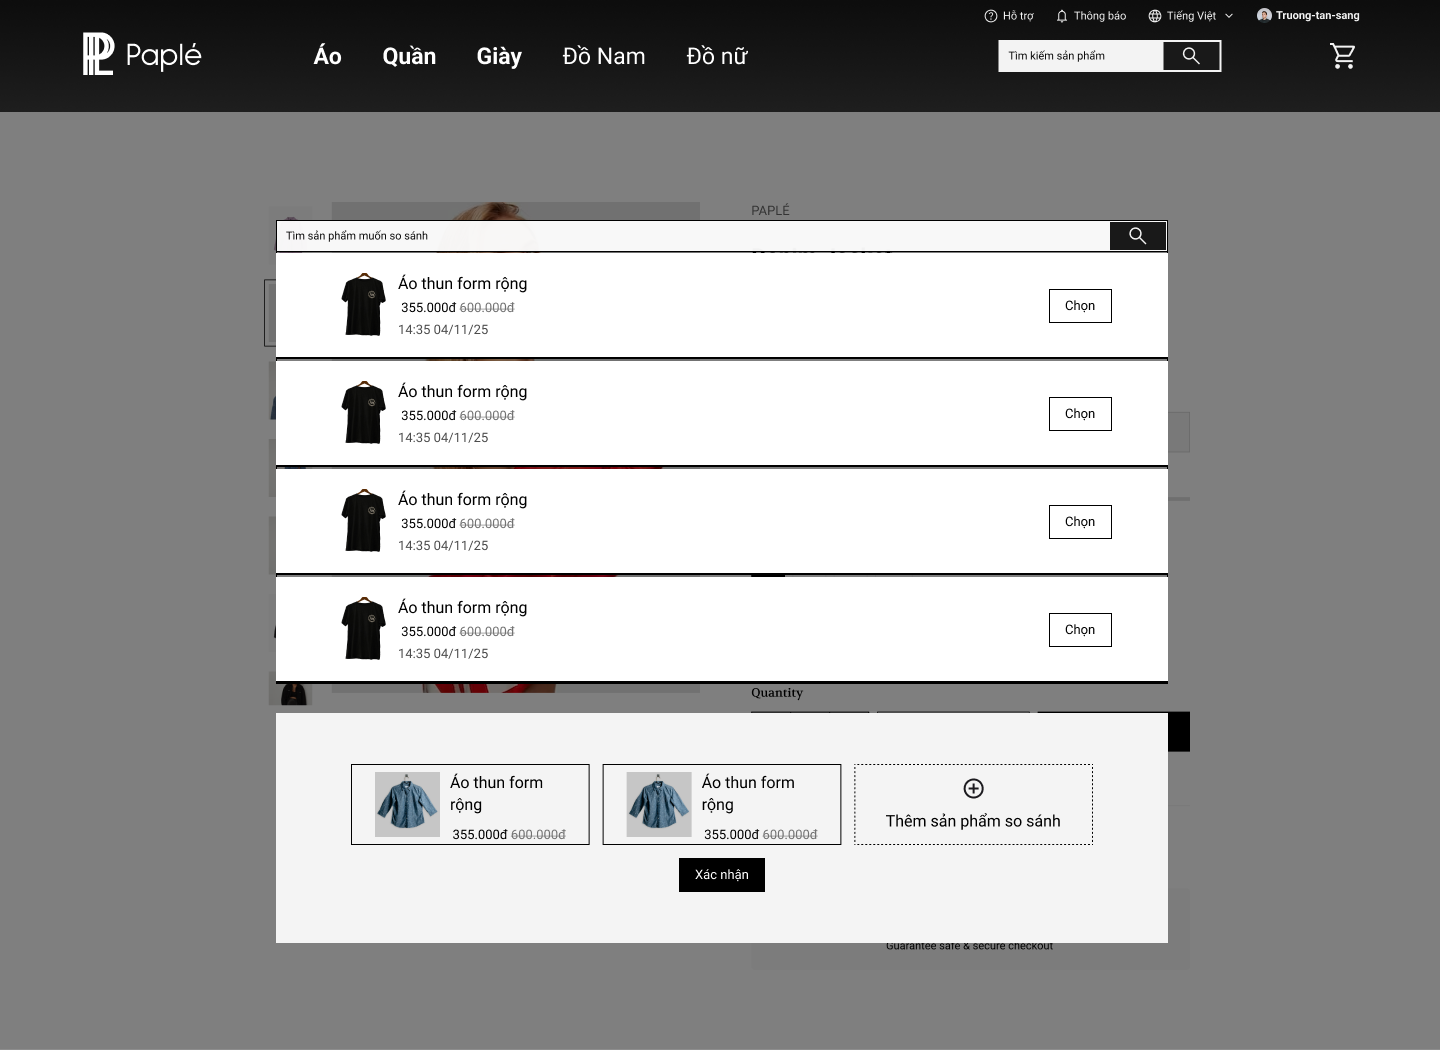
\includegraphics[width=1\textwidth]{Images/MockUp/Customer/Comparison/_1.png}
    \vspace{0.5cm}
    \caption{Giao diện So sánh Sản phẩm}
    \label{fig: Giao diện So sánh Sản phẩm}
\end{figure}
\noindent\textbf{Các bước chọn sản phẩm để so sánh:}
\begin{enumerate}
    \item Từ trang chi tiết sản phẩm, chọn chức năng \textit{So sánh} để thêm sản phẩm hiện tại vào bảng so sánh.
    \item Sử dụng ô tìm kiếm để chọn thêm các sản phẩm cần so sánh.
    \item Tại mỗi sản phẩm, nhấn \textit{Thêm vào so sánh} để đưa sản phẩm vào danh sách so sánh.
    \item Mở màn hình \textit{So sánh} để xem bảng so sánh hiển thị các thuộc tính: giá, kích cỡ, màu sắc/chất liệu, đánh giá, mô tả.
    \item Tùy chọn \textit{Xóa} một sản phẩm khỏi trang so sánh nếu không cần thiết, hoặc \textit{Thêm vào giỏ hàng}/\textit{Mua ngay} từ bảng so sánh.
\end{enumerate}
\begin{figure}[H]
    \centering
    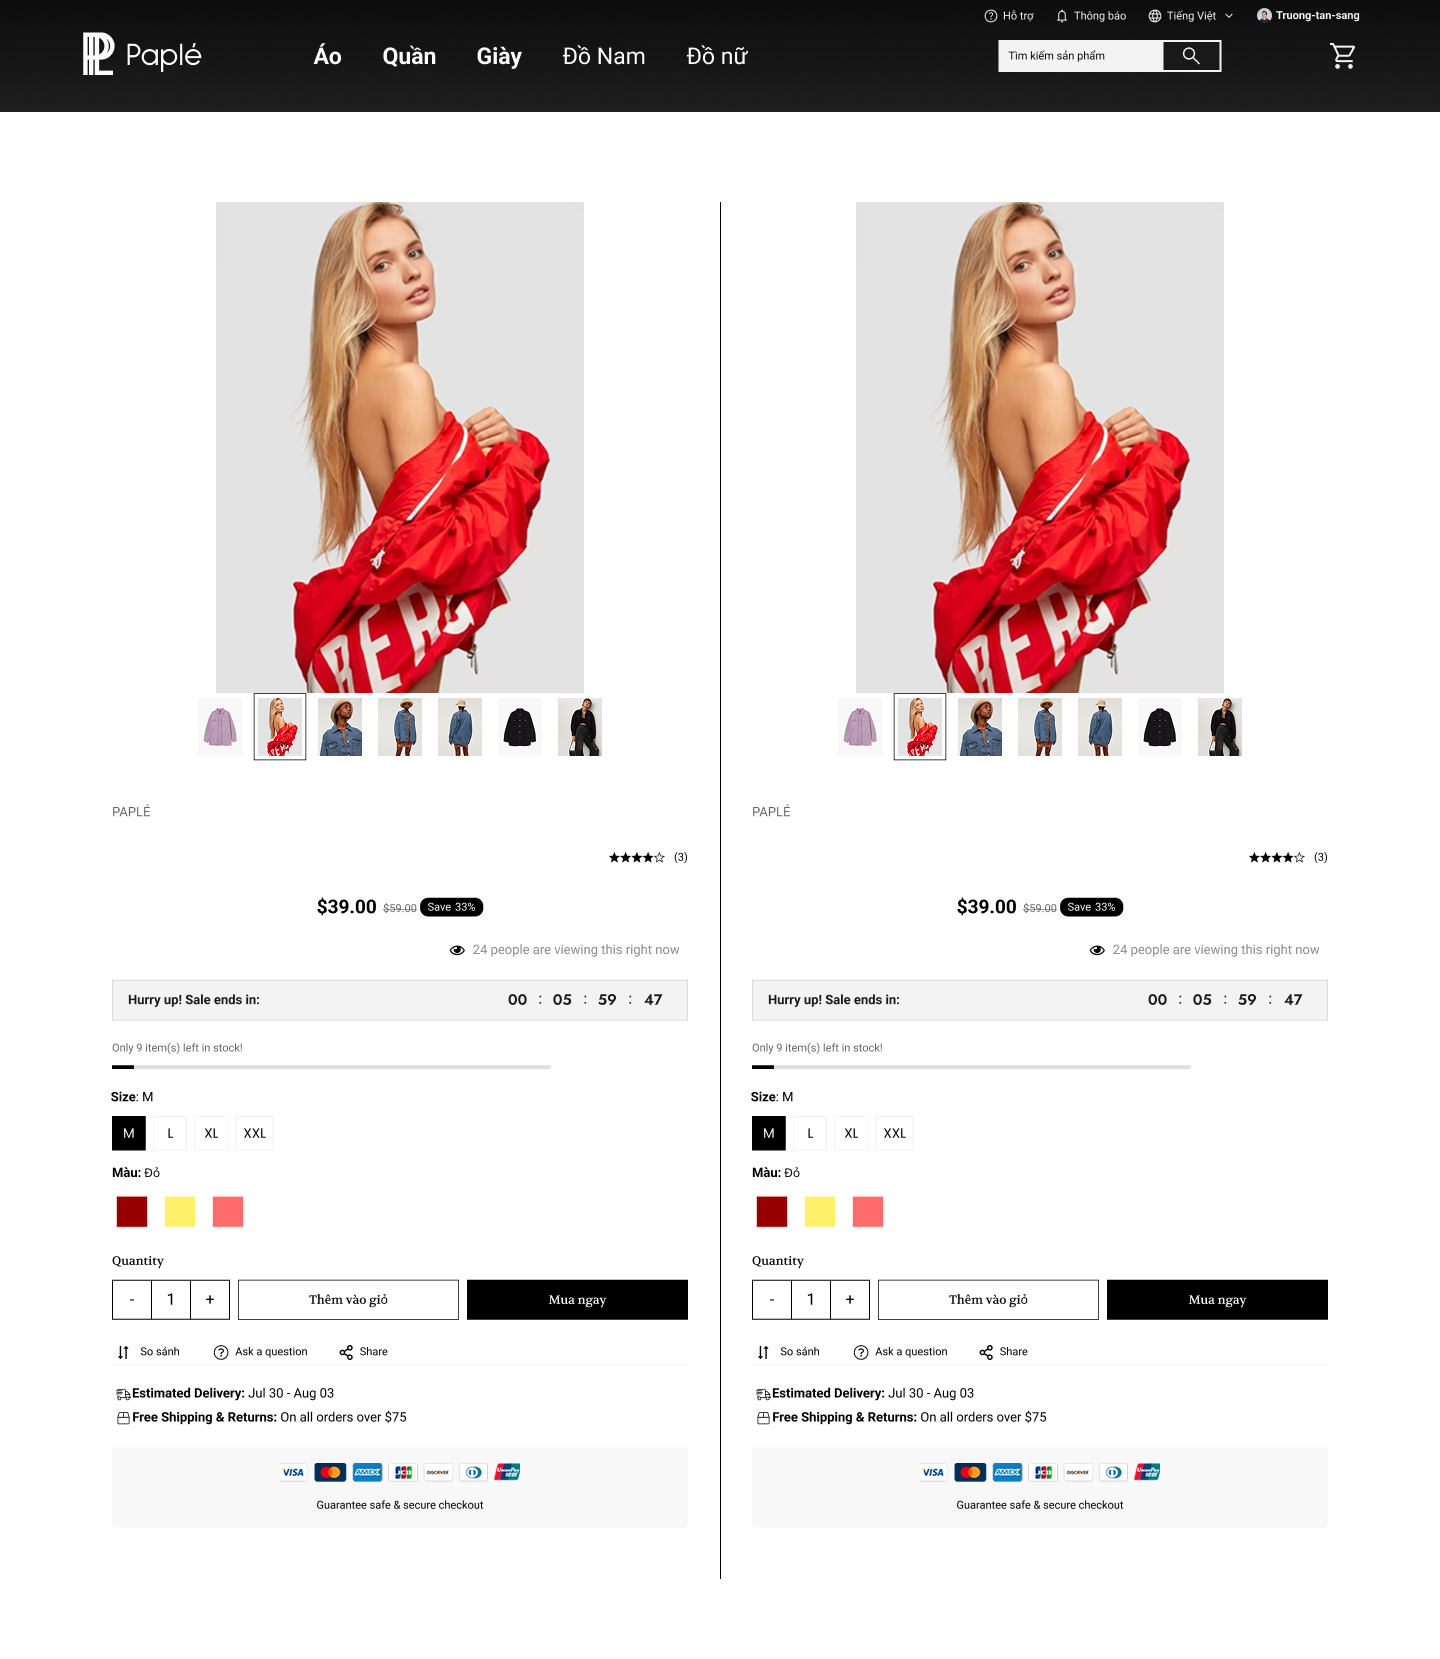
\includegraphics[width=1\textwidth]{Images/MockUp/Customer/Comparison/_2.png}
    \vspace{0.5cm}
    \caption{Các bước chọn sản phẩm để so sánh}
    \label{fig: Các bước chọn sản phẩm để so sánh}
\end{figure}
\noindent\textbf{Các thao tác chính:} So sánh thông tin chi tiết các sản phẩm (giá, kích cỡ, chất liệu, đánh giá), xóa sản phẩm khỏi bảng so sánh, thêm sản phẩm vào giỏ hàng từ bảng so sánh, và mua ngay sản phẩm được chọn.
\subsubsubsection {Trang cá nhân}
\begin{enumerate}
    \item Trang thông tin cá nhân:
          \begin{figure}[H]
              \centering
              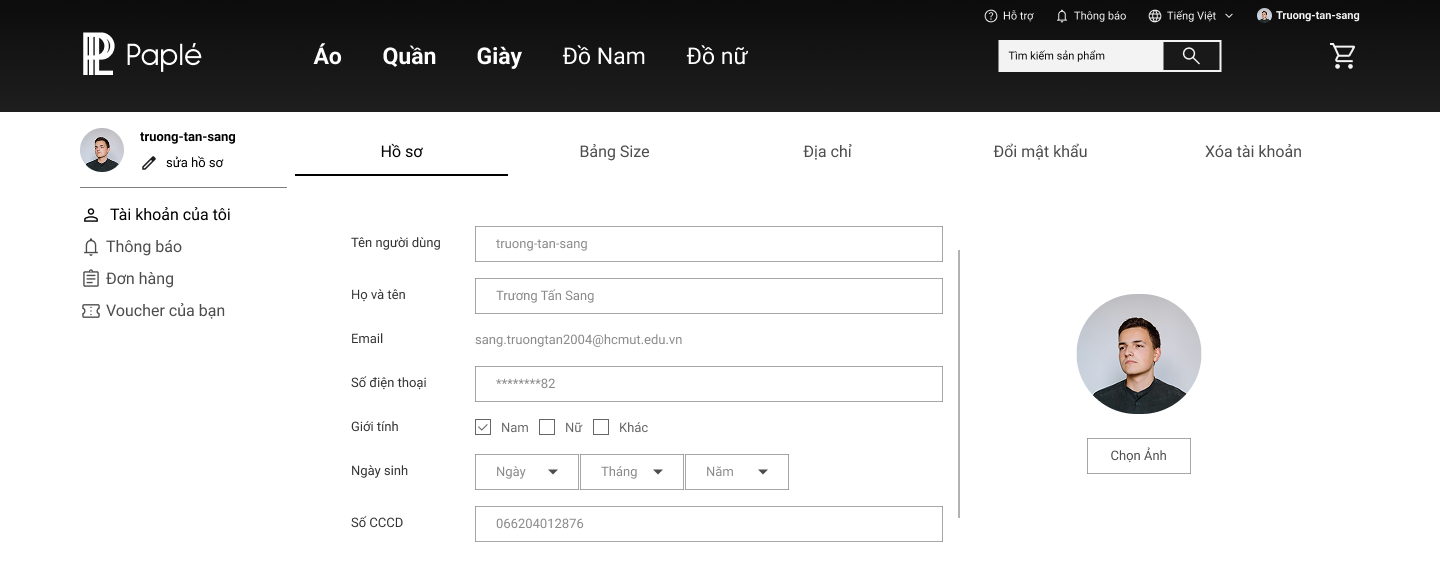
\includegraphics[width=1\textwidth]{Images/MockUp/Customer/Profile/Profile.png}
              \vspace{0.5cm}
              \caption{Giao diện trang thông tin cá nhân}
              \label{fig: Giao diện trang thông tin cá nhân}
          \end{figure}
          \noindent\textbf{Các thao tác chính:} Xem và chỉnh sửa thông tin cá nhân (tên, email, số điện thoại, ảnh đại diện), quản lý các địa chỉ, xem lịch sử giao dịch, và cập nhật thông tin tài khoản.

    \item Trang kích cỡ:
          \begin{figure}[H]
              \centering
              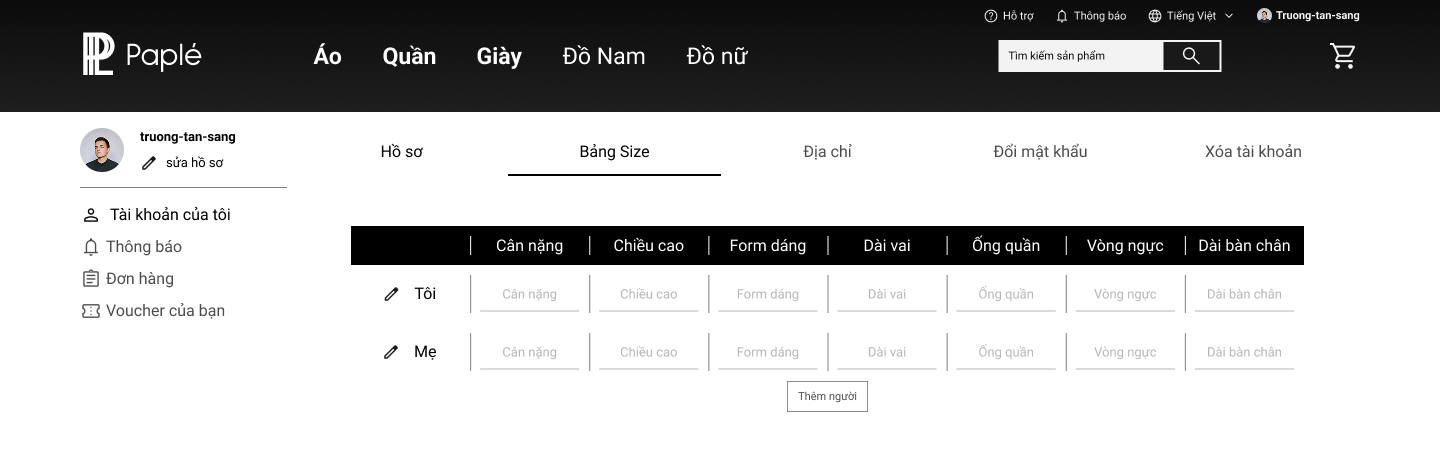
\includegraphics[width=1\textwidth]{Images/MockUp/Customer/Profile/Size.png}
              \vspace{0.5cm}
              \caption{Giao diện trang kích cỡ}
              \label{fig: Giao diện trang kích cỡ}
          \end{figure}
          \noindent\textbf{Các thao tác chính:} Lưu và quản lý thông tin kích cỡ cơ thể cho các loại sản phẩm khác nhau, cập nhật số đo cơ thể, và sử dụng thông tin kích cỡ để gợi ý sản phẩm phù hợp.

    \item Trang quản lý địa chỉ:
          \begin{figure}[H]
              \centering
              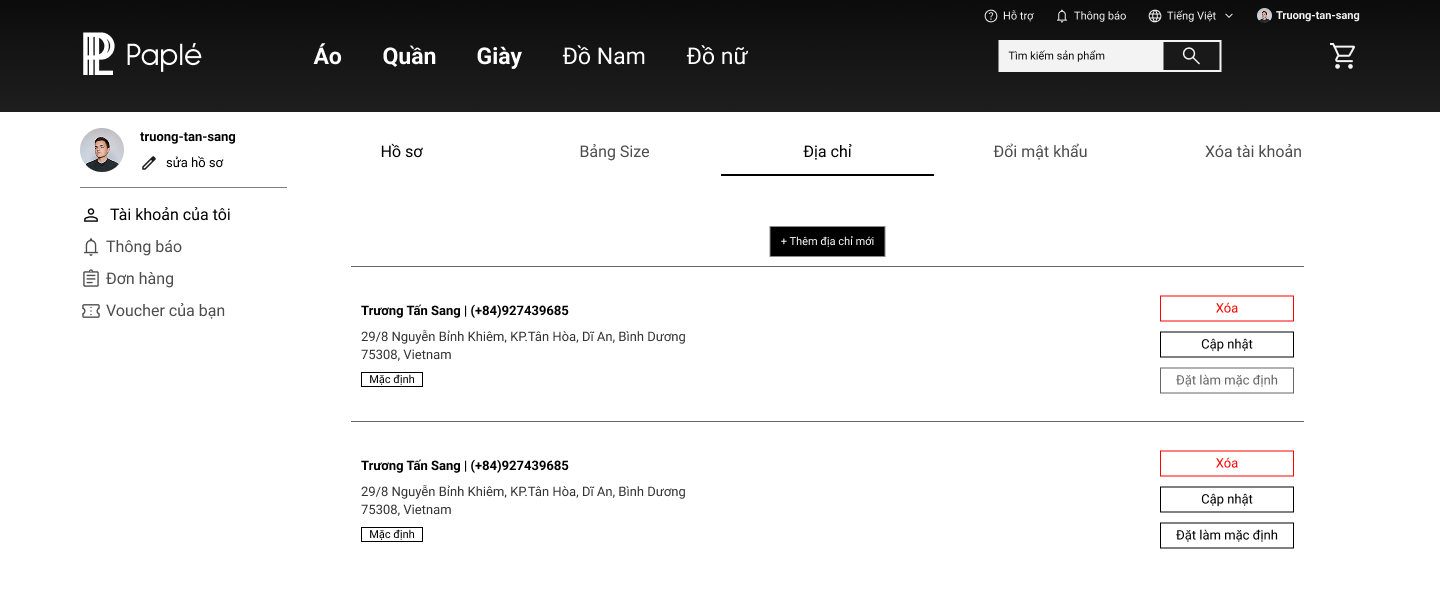
\includegraphics[width=1\textwidth]{Images/MockUp/Customer/Profile/Address.png}
              \vspace{0.5cm}
              \caption{Giao diện trang quản lý địa chỉ}
              \label{fig: Giao diện trang quản lý địa chỉ}
          \end{figure}
          \noindent\textbf{Các thao tác chính:} Thêm, chỉnh sửa và xóa địa chỉ giao hàng, đặt địa chỉ mặc định, xem danh sách đầy đủ các địa chỉ đã lưu, và nhanh chóng chọn địa chỉ trong quá trình thanh toán.

    \item Trang đổi mật khẩu:
          \begin{figure}[H]
              \centering
              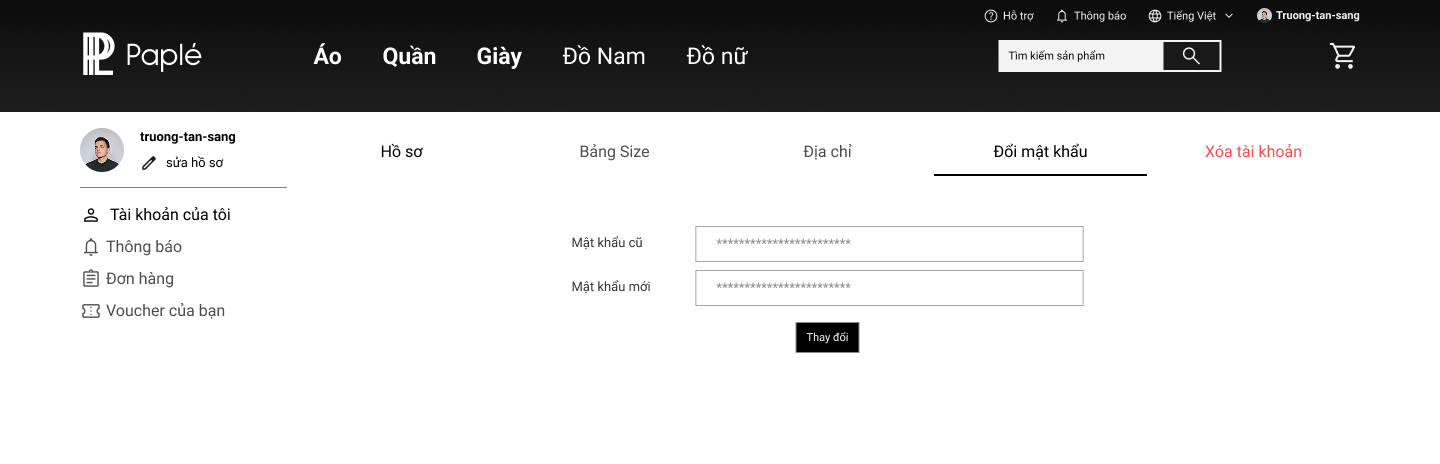
\includegraphics[width=1\textwidth]{Images/MockUp/Customer/Profile/Change Password.png}
              \vspace{0.5cm}
              \caption{Giao diện trang đổi mật khẩu}
              \label{fig: Giao diện trang đổi mật khẩu}
          \end{figure}
          \noindent\textbf{Các thao tác chính:} Nhập mật khẩu cũ, nhập mật khẩu mới, xác nhận mật khẩu mới, và cập nhật mật khẩu để bảo vệ tài khoản.

    \item Trang xóa tài khoản:
          \begin{figure}[H]
              \centering
              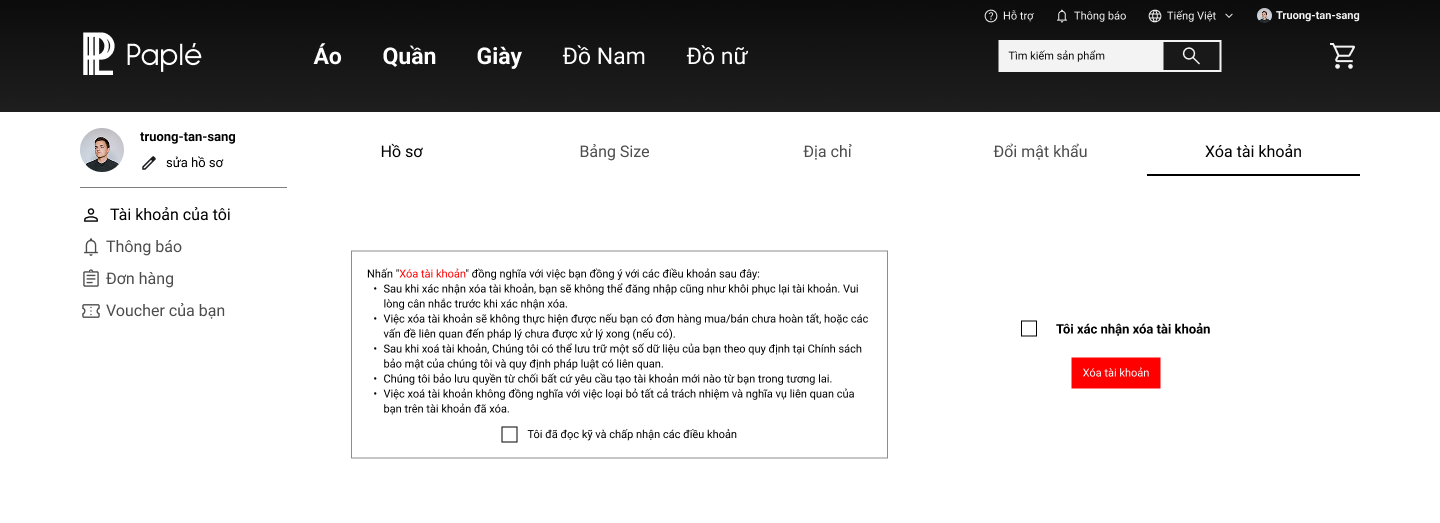
\includegraphics[width=1\textwidth]{Images/MockUp/Customer/Profile/Delete Account.png}
              \vspace{0.5cm}
              \caption{Giao diện trang xóa tài khoản}
              \label{fig: Giao diện trang xóa tài khoản}
          \end{figure}
          \noindent\textbf{Các thao tác chính:} Xác nhận yêu cầu xóa tài khoản, đọc cảnh báo và hậu quả của việc xóa tài khoản vĩnh viễn, và hoàn tất quy trình xóa tài khoản.
\end{enumerate}
\subsubsubsection {Quản lý đơn hàng}
\begin{enumerate}
    \item Tất cả đơn hàng:
          \begin{figure}[H]
              \centering
              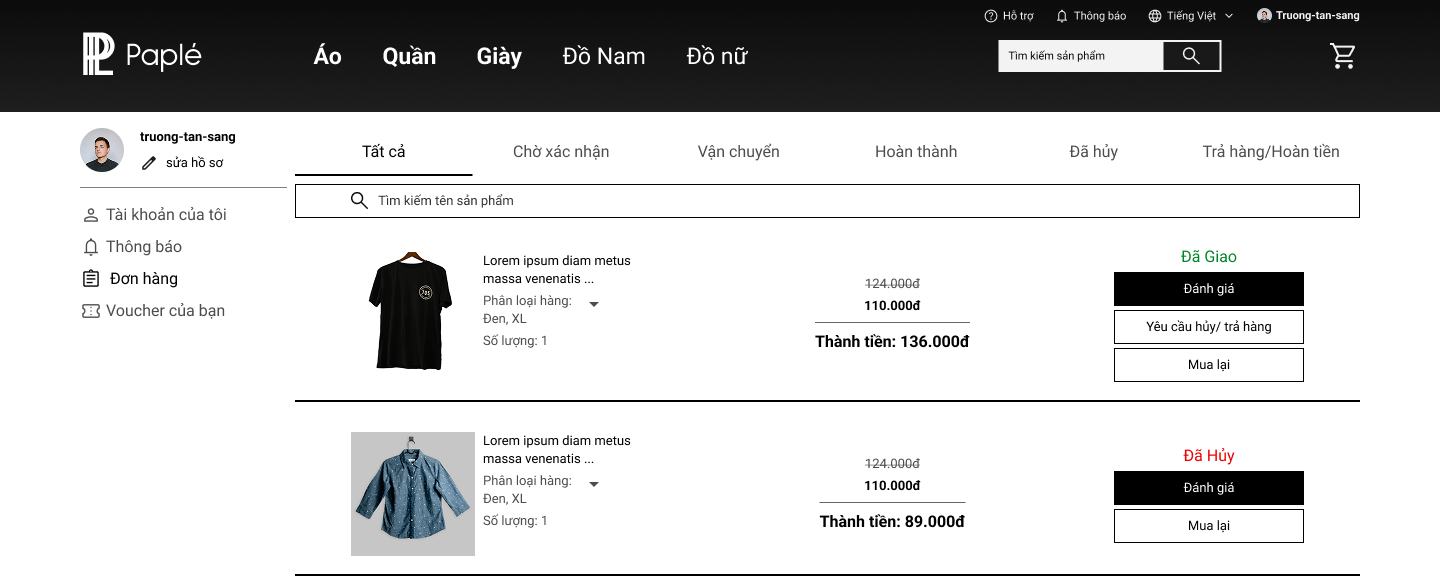
\includegraphics[width=1\textwidth]{Images/MockUp/Customer/Orders/All.png}
              \vspace{0.5cm}
              \caption{Giao diện xem tất cả đơn hàng}
              \label{fig: Giao diện xem tất cả đơn hàng}
          \end{figure}
          \noindent\textbf{Các thao tác chính:} Xem danh sách toàn bộ đơn hàng, lọc theo trạng thái, sắp xếp theo ngày, tìm kiếm đơn hàng, xem chi tiết từng đơn, và thực hiện các hành động liên quan (hủy, trả hàng, theo dõi).

    \item Chi tiết đơn hàng:
          \begin{figure}[H]
              \centering
              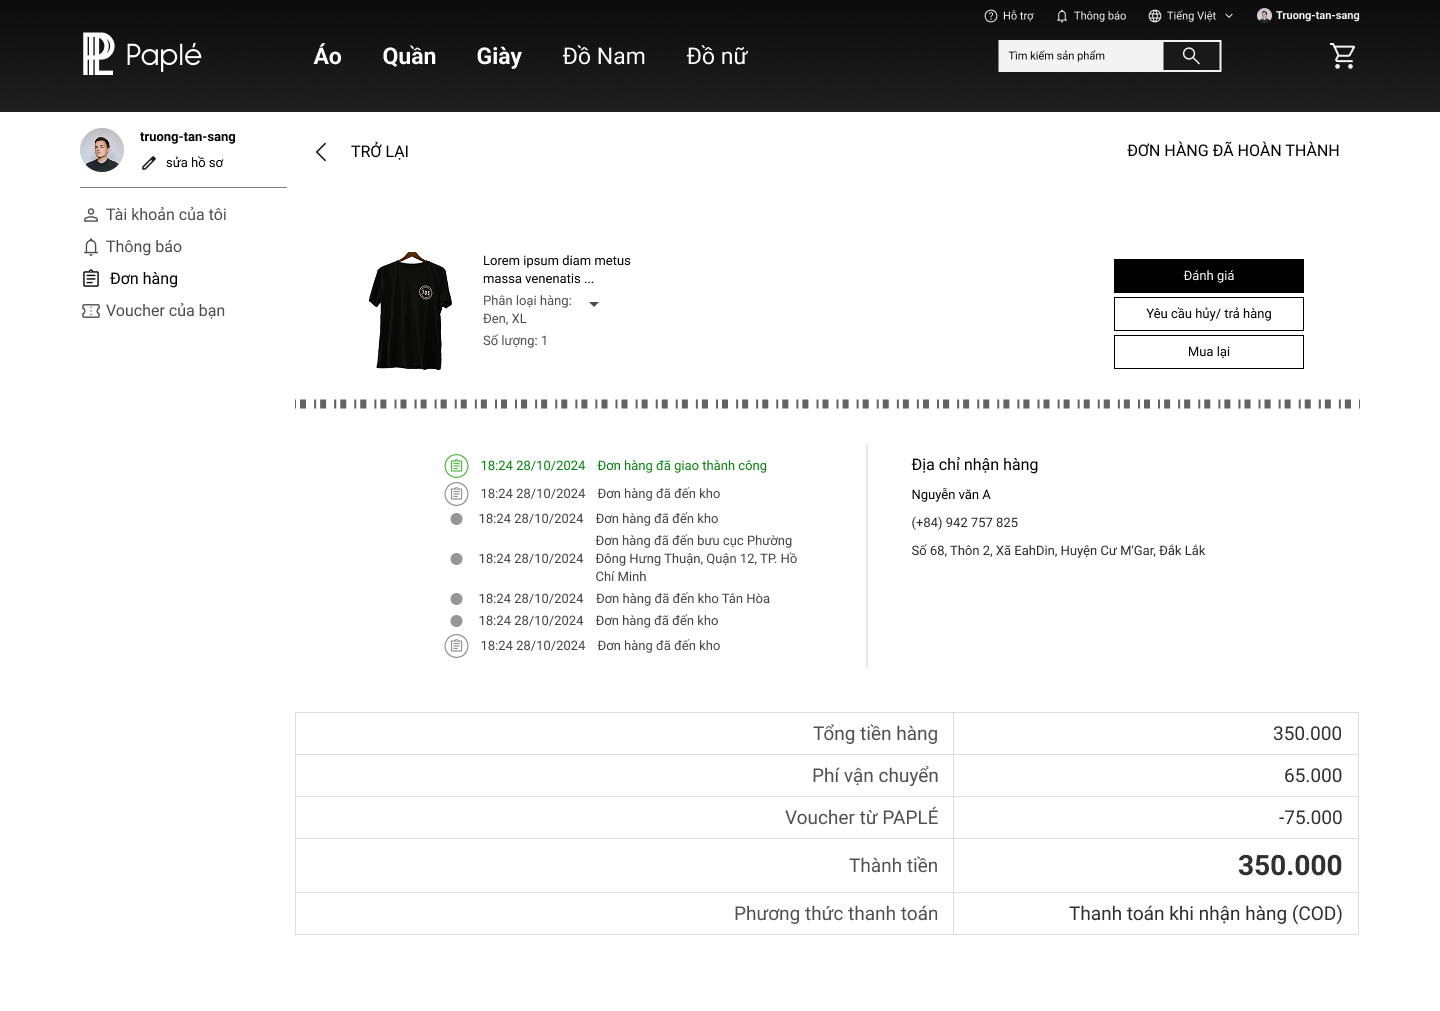
\includegraphics[width=1\textwidth]{Images/MockUp/Customer/Orders/Details.png}
              \vspace{0.5cm}
              \caption{Giao diện chi tiết đơn hàng}
              \label{fig: Giao diện chi tiết đơn hàng}
          \end{figure}
          \noindent\textbf{Các thao tác chính:} Xem thông tin chi tiết đơn hàng bao gồm ngày đặt, trạng thái hiện tại, danh sách sản phẩm (tên, số lượng, giá, màu sắc, kích cỡ), thông tin người nhận (tên, địa chỉ giao hàng, số điện thoại), phương thức thanh toán, thông tin voucher đã áp dụng, chi phí vận chuyển, tổng tiền thanh toán, lịch sử cập nhật trạng thái đơn hàng, và các tùy chọn hành động (hủy đơn, yêu cầu trả hàng, theo dõi vận chuyển).
    \item Đánh giá đơn hàng:
          \begin{figure}[H]
              \centering
              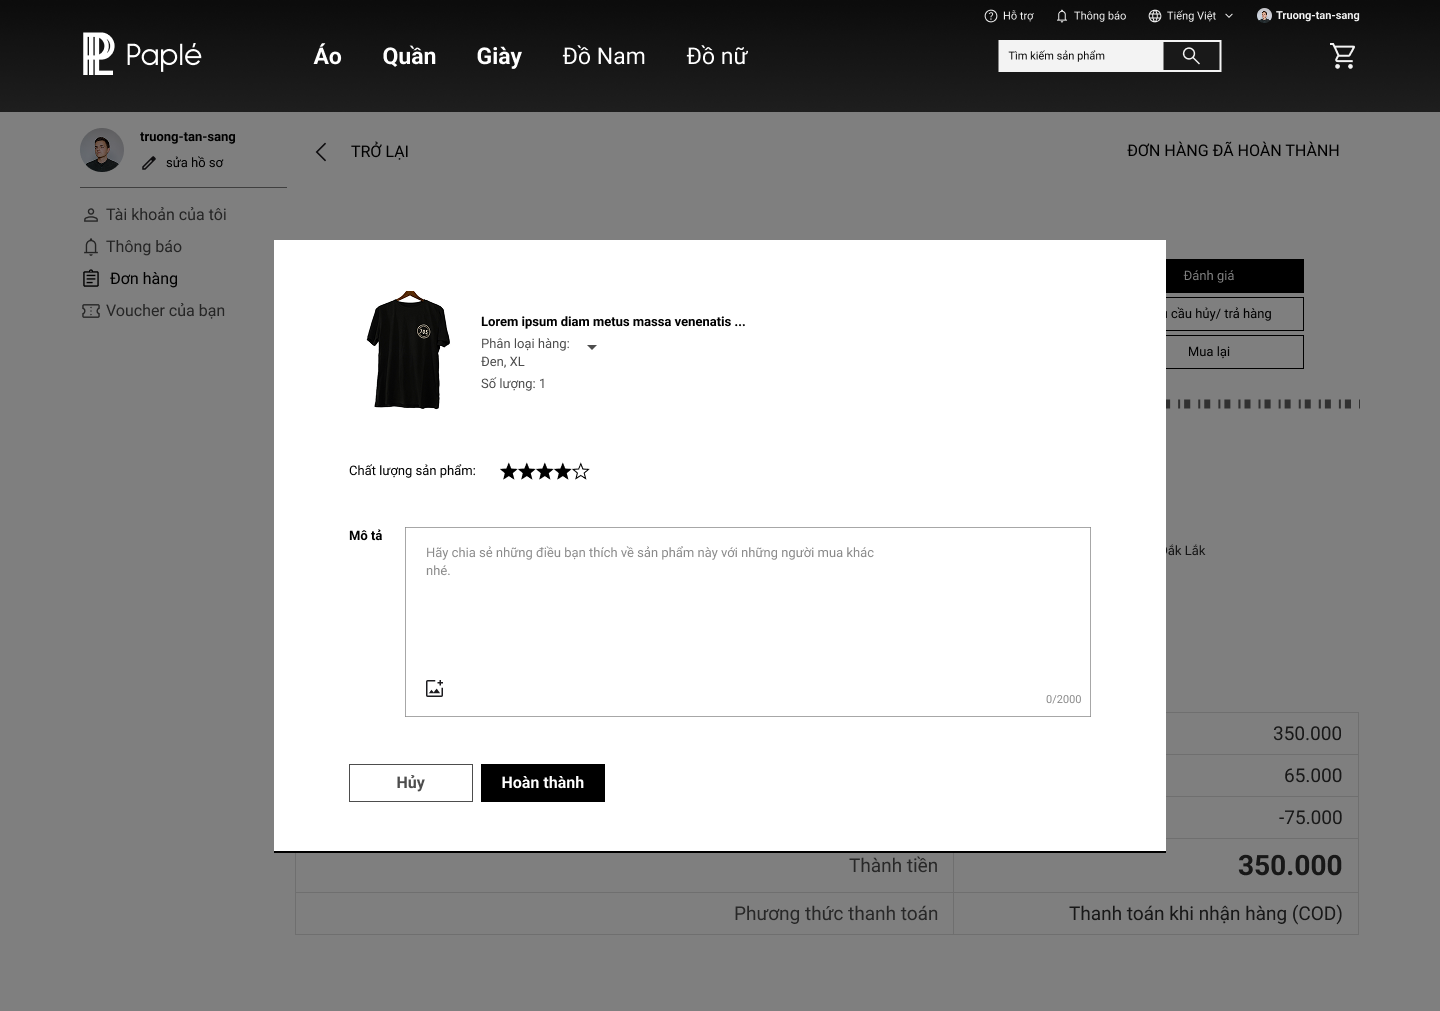
\includegraphics[width=1\textwidth]{Images/MockUp/Customer/Orders/Review.png}
              \vspace{0.5cm}
              \caption{Giao diện đánh giá đơn hàng}
              \label{fig: Giao diện đánh giá đơn hàng}
          \end{figure}
          \noindent\textbf{Các thao tác chính:} Xem lại chi tiết sản phẩm vừa mua, chọn số sao đánh giá, nhập nội dung nhận xét, đính kèm hình ảnh minh họa, gửi đánh giá, và xem danh sách các đánh giá đã tạo.
          \newpage
    \item Hủy/trả đơn hàng:
          \begin{figure}[H]
              \centering
              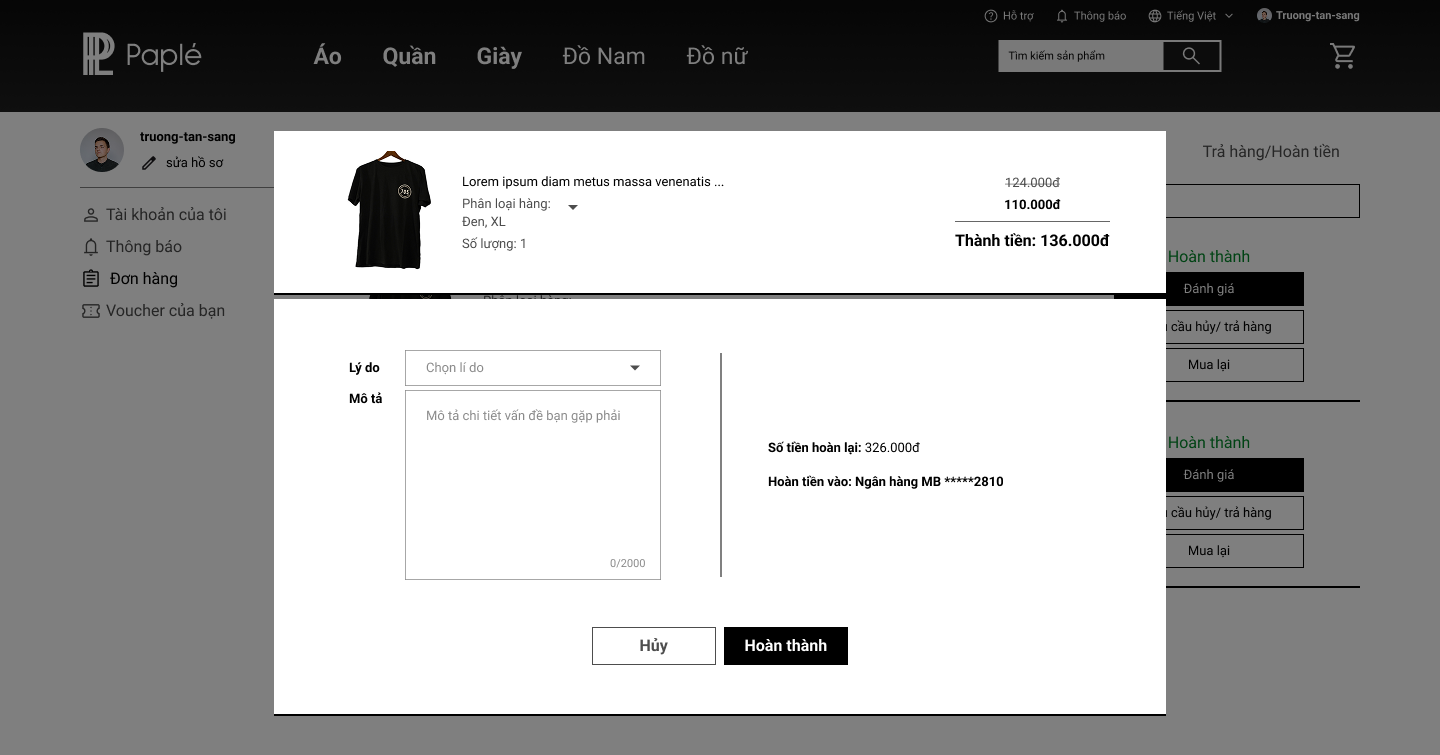
\includegraphics[width=1\textwidth]{Images/MockUp/Customer/Orders/Cancel+Return request.png}
              \vspace{0.5cm}
              \caption{Giao diện hủy/trả đơn hàng}
              \label{fig: Giao diện hủy/trả đơn hàng}
          \end{figure}
          \noindent\textbf{Các thao tác chính:} Tạo yêu cầu hủy đơn hàng hoặc trả hàng, chọn lý do hủy/trả hàng, mô tả chi tiết vấn đề gặp phải, đính kèm hình ảnh/video minh họa (đối với trả hàng), gửi yêu cầu.

\end{enumerate}
\subsubsubsection {Thông báo}
\begin{enumerate}
    \item Thông báo cập nhật đơn hàng:
          \begin{figure}[H]
              \centering
              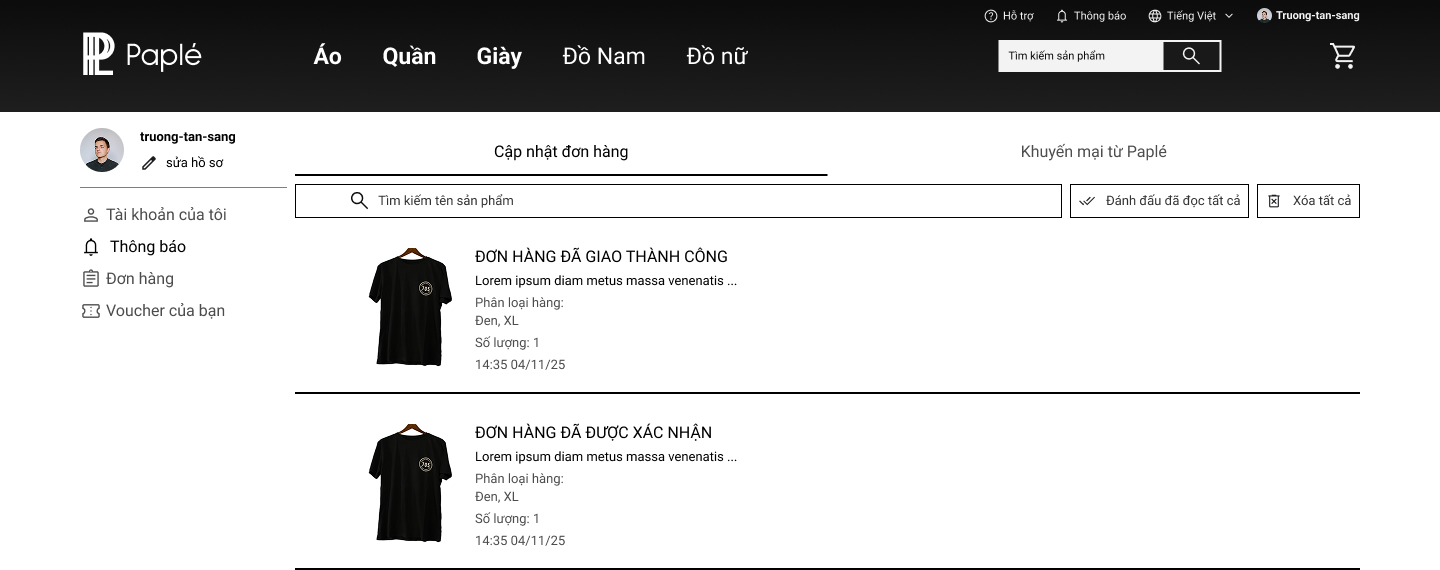
\includegraphics[width=1\textwidth]{Images/MockUp/Customer/Notifications/Order updates.png}
              \vspace{0.5cm}
              \caption{Giao diện thông báo cập nhật đơn hàng}
              \label{fig: Giao diện thông báo cập nhật đơn hàng}
          \end{figure}
          \noindent\textbf{Các thao tác chính:} Hiển thị thông báo về trạng thái đơn hàng (xác nhận, thanh toán, đang giao, đã giao), xem chi tiết thông báo, đánh dấu đã đọc, và xóa thông báo.

    \item Thông báo khuyến mãi:
          \begin{figure}[H]
              \centering
              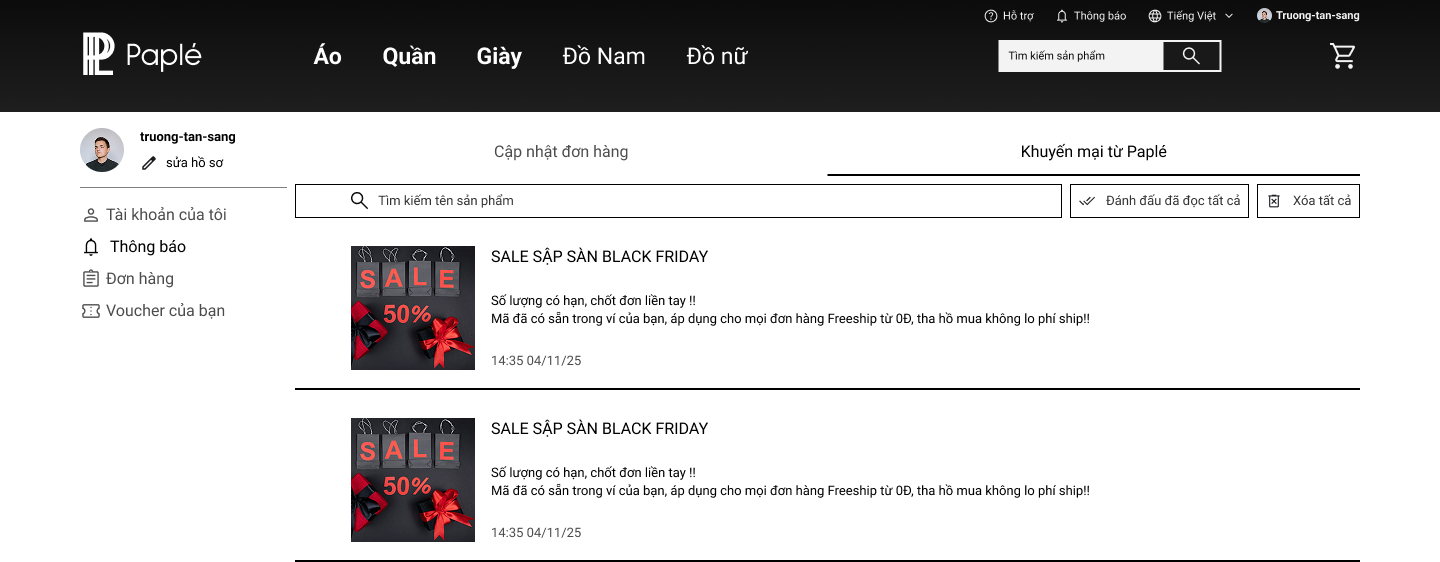
\includegraphics[width=1\textwidth]{Images/MockUp/Customer/Notifications/Sales.png}
              \vspace{0.5cm}
              \caption{Giao diện thông báo khuyến mãi}
              \label{fig: Giao diện thông báo khuyến mãi}
          \end{figure}
          \noindent\textbf{Các thao tác chính:} Hiển thị thông báo về khuyến mãi, giảm giá, và sản phẩm mới, xem chi tiết chương trình khuyến mãi, lưu thông báo, và điều hướng đến sản phẩm liên quan.
\end{enumerate}

\subsubsection{Thiết kế giao diện cho quản trị viên}
\subsubsubsection {Trang tổng quan (Dashboard)}
\begin{figure}[H]
    \centering
    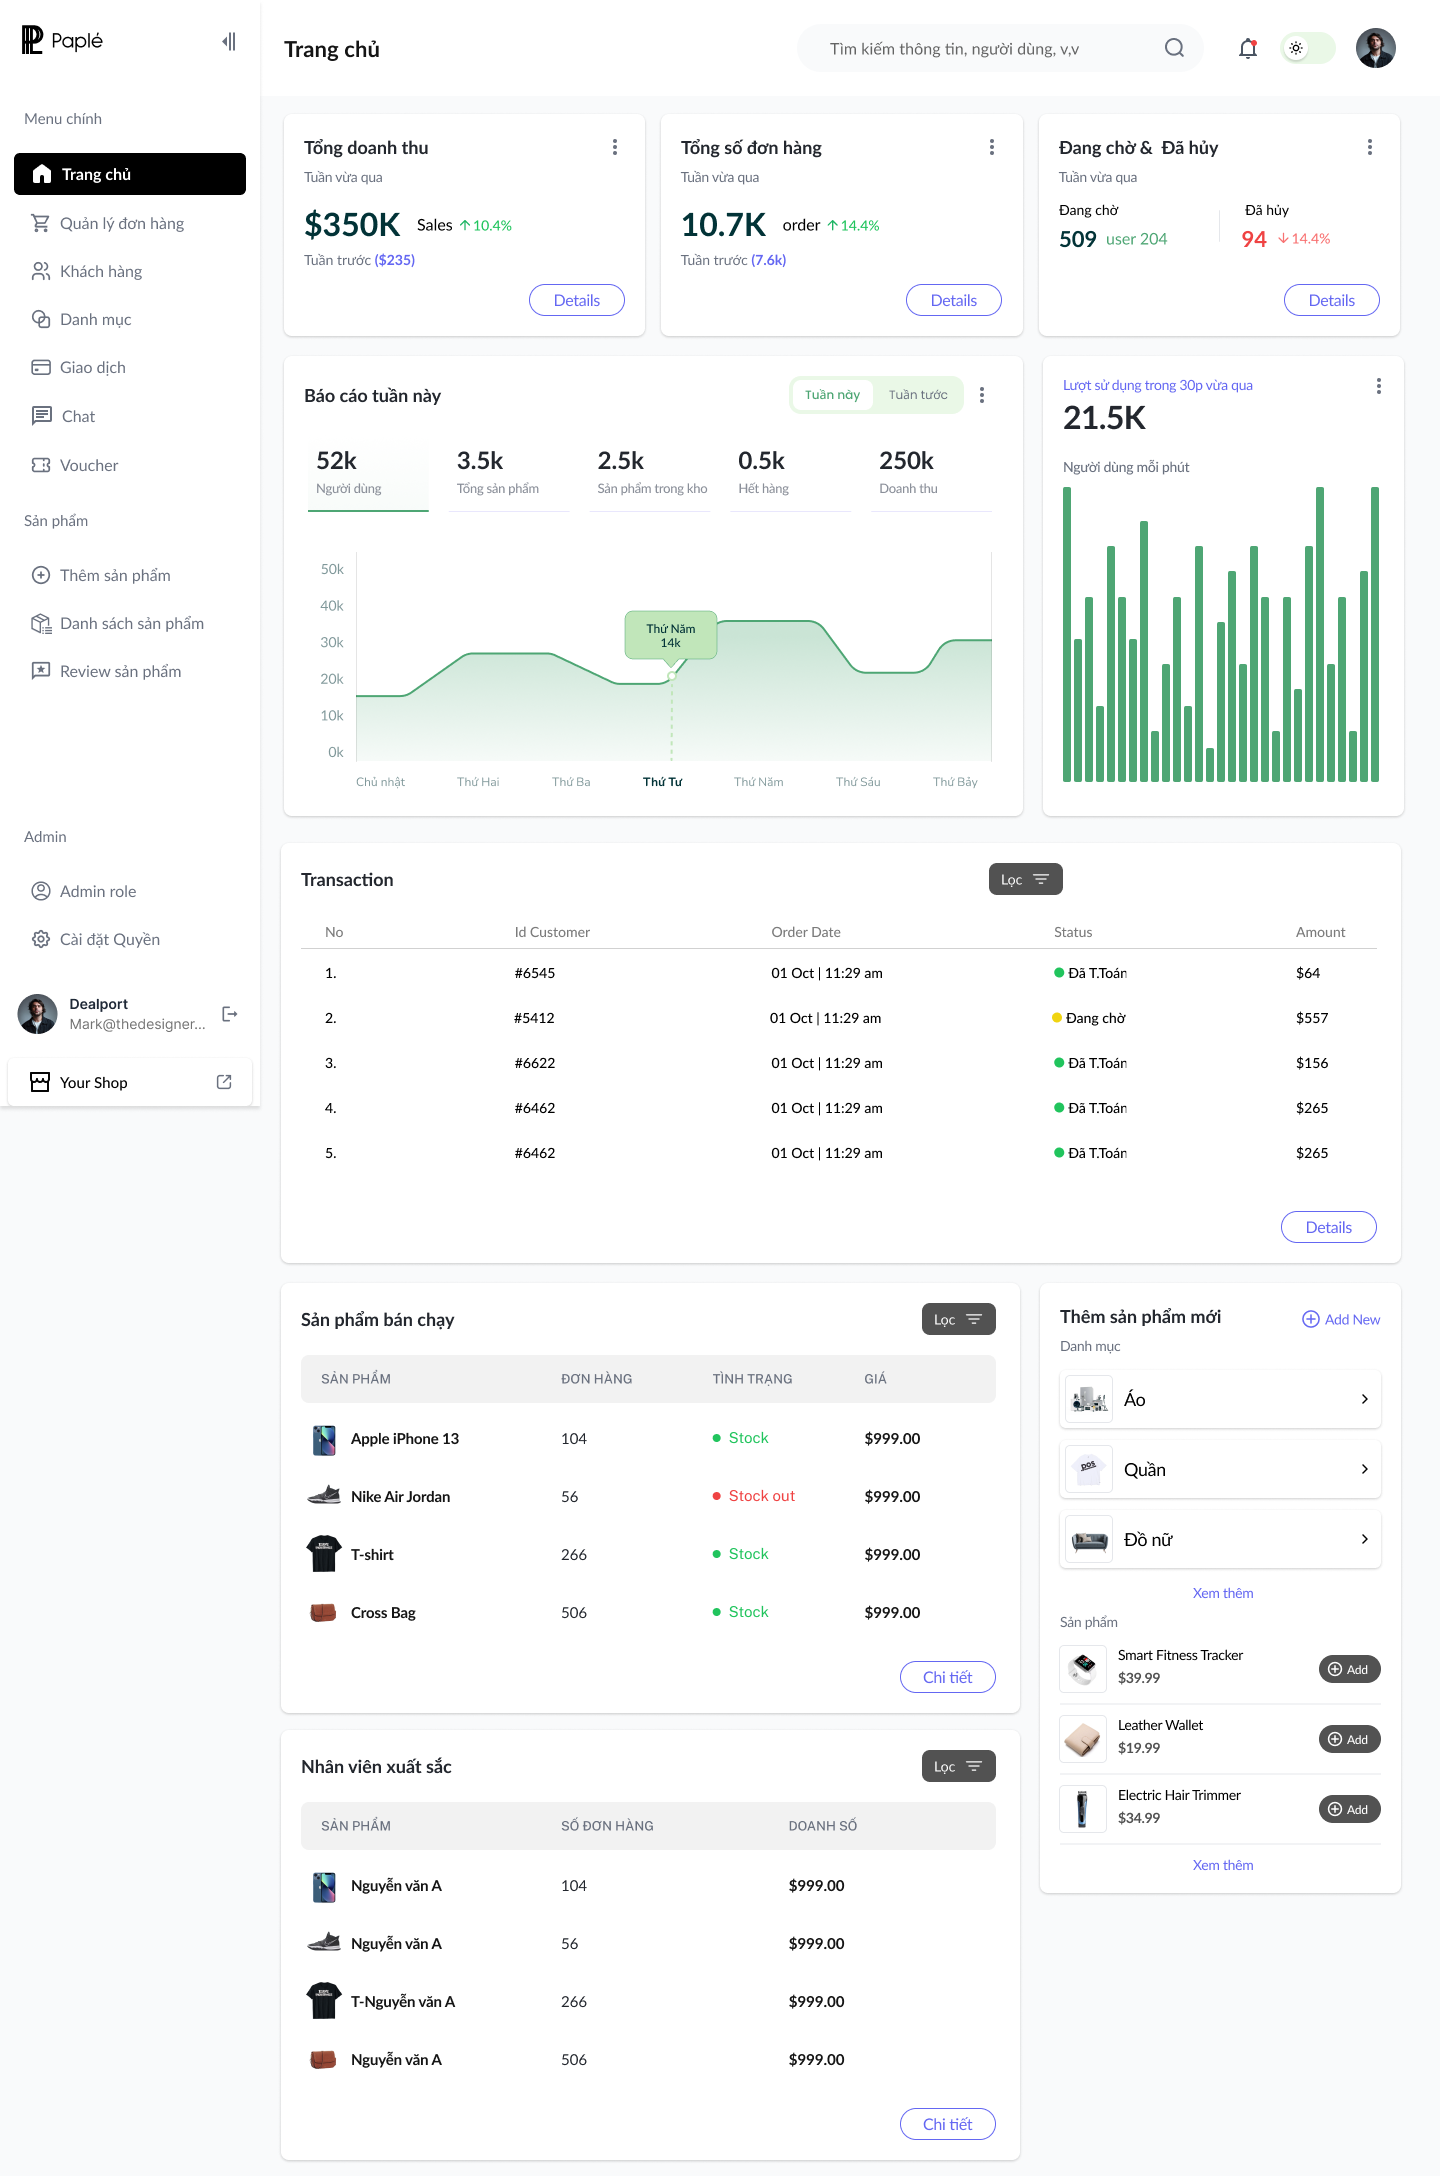
\includegraphics[width=0.8\textwidth]{Images/MockUp/Admin/Dashboard.png}
    \vspace{0.5cm}
    \caption{Giao diện trang tổng quan}
    \label{fig: Giao diện trang tổng quan}
\end{figure}
\noindent\textbf{Các thao tác chính:} Xem tổng quan về doanh thu, số đơn hàng, số khách hàng mới, xem các biểu đồ thống kê, và truy cập nhanh đến các chức năng quản lý chính.

\subsubsubsection {Quản lý đơn hàng}
\begin{figure}[H]
    \centering
    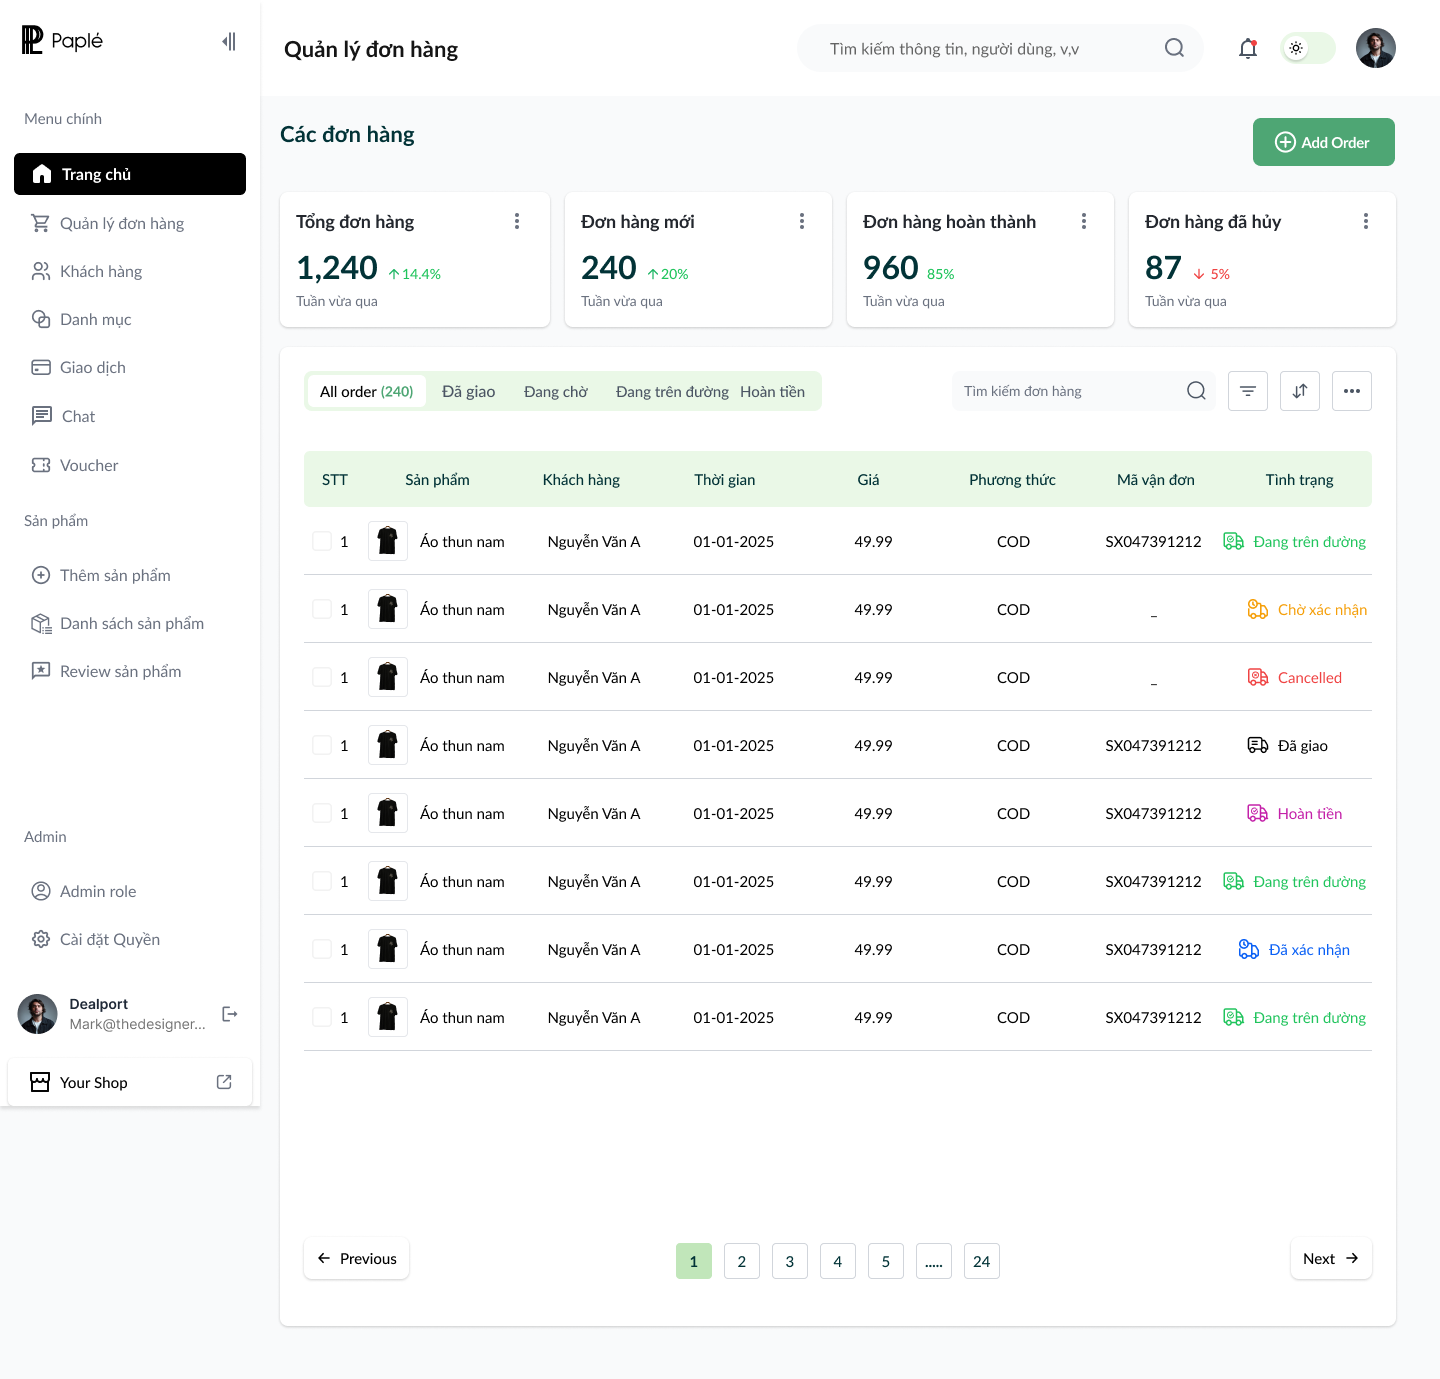
\includegraphics[width=1\textwidth]{Images/MockUp/Admin/Order Management.png}
    \vspace{0.5cm}
    \caption{Giao diện quản lý đơn hàng}
    \label{fig: Giao diện quản lý đơn hàng}
\end{figure}
\noindent\textbf{Các thao tác chính:} Xem danh sách tất cả đơn hàng, lọc theo trạng thái, cập nhật trạng thái đơn hàng, xác nhận thanh toán, và quản lý vận chuyển.

\subsubsubsection {Chi tiết đơn hàng (Admin)}
\begin{enumerate}
    \item Đơn hàng bình thường:
          \begin{figure}[H]
              \centering
              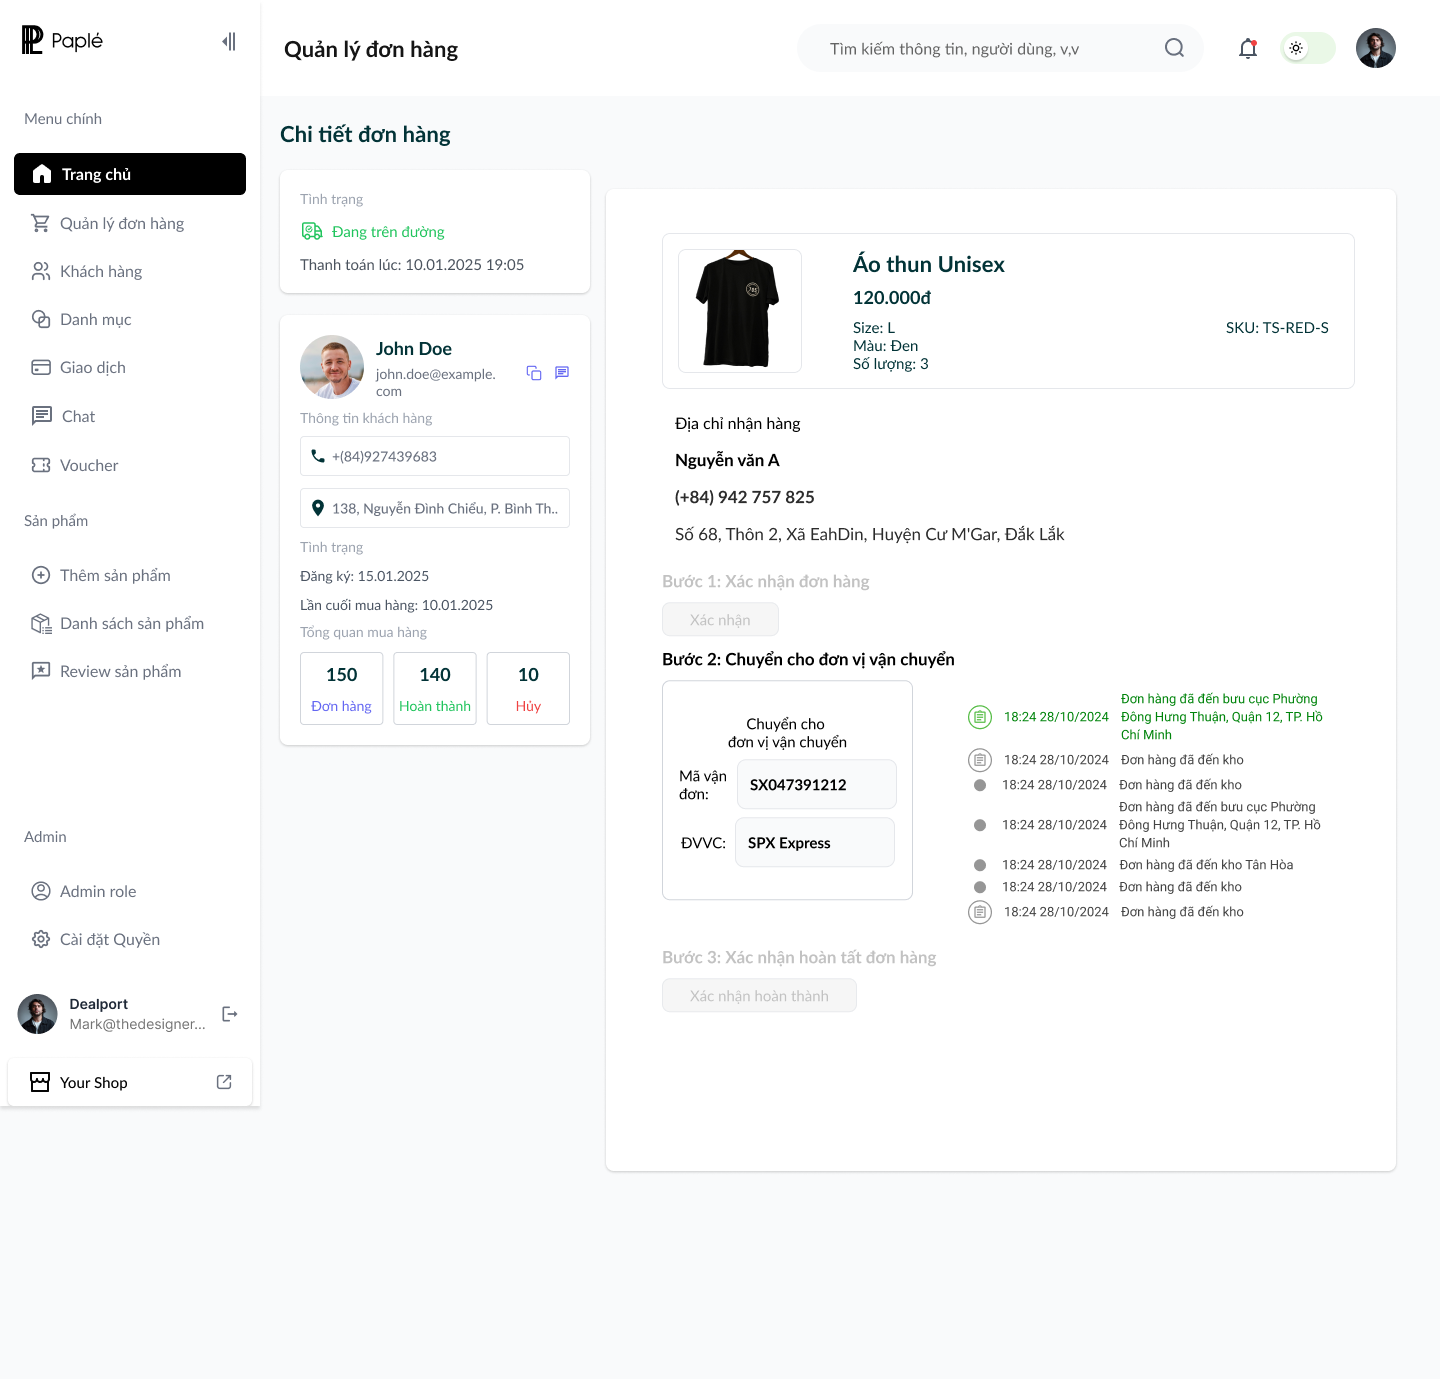
\includegraphics[width=1\textwidth]{Images/MockUp/Admin/Order Detail.png}
              \vspace{0.5cm}
              \caption{Giao diện chi tiết đơn hàng bình thường (Admin)}
              \label{fig: Giao diện chi tiết đơn hàng bình thường (Admin)}
          \end{figure}
          \noindent\textbf{Mô tả:} Hiển thị ngày đặt, trạng thái, khách hàng, địa chỉ giao, phương thức thanh toán, chi tiết sản phẩm (biến thể, số lượng, giá), phí vận chuyển, voucher, tổng tiền, lịch sử cập nhật trạng thái. Cho phép xác nhận, đóng gói, bàn giao vận chuyển, cập nhật trạng thái.

          \newpage
    \item Đơn hàng yêu cầu đổi/trả:
          \begin{figure}[H]
              \centering
              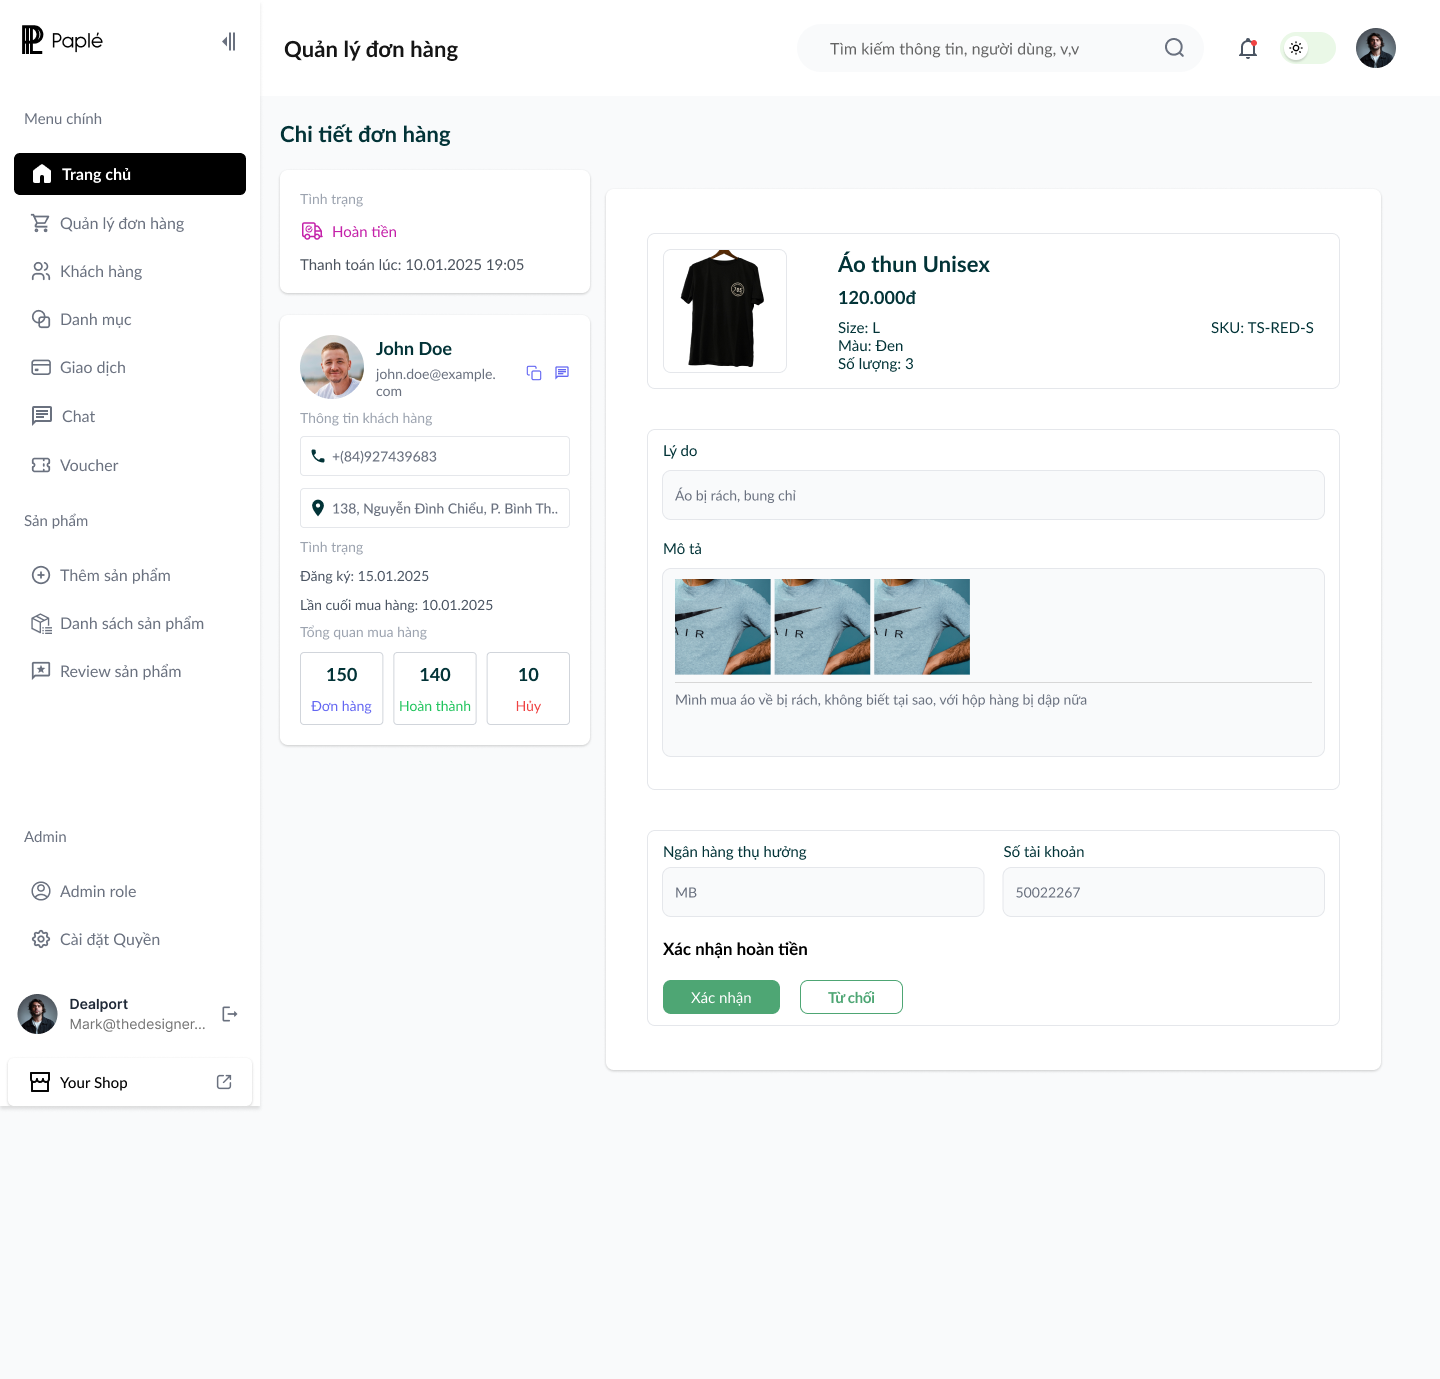
\includegraphics[width=1\textwidth]{Images/MockUp/Admin/Returned Order 1.png}
              \vspace{0.5cm}
              \caption{Giao diện chi tiết đơn hàng yêu cầu đổi/trả (Admin)}
              \label{fig: Giao diện chi tiết đơn hàng yêu cầu đổi/trả (Admin)}
          \end{figure}
          \noindent\textbf{Mô tả:} Hiển thị thông tin đơn hàng yêu cầu đổi/trả bao gồm lý do trả hàng, hình ảnh/video minh họa từ khách hàng, thông tin đơn hàng gốc. Từ trang này, quản trị viên có 2 lựa chọn:
          \begin{itemize}
              \item \textbf{Xác nhận hoàn tiền:} Khi chấp nhận yêu cầu, hệ thống sẽ mở modal thanh toán để xác nhận thực hiện hoàn tiền cho khách hàng.
                    \begin{figure}[H]
                        \centering
                        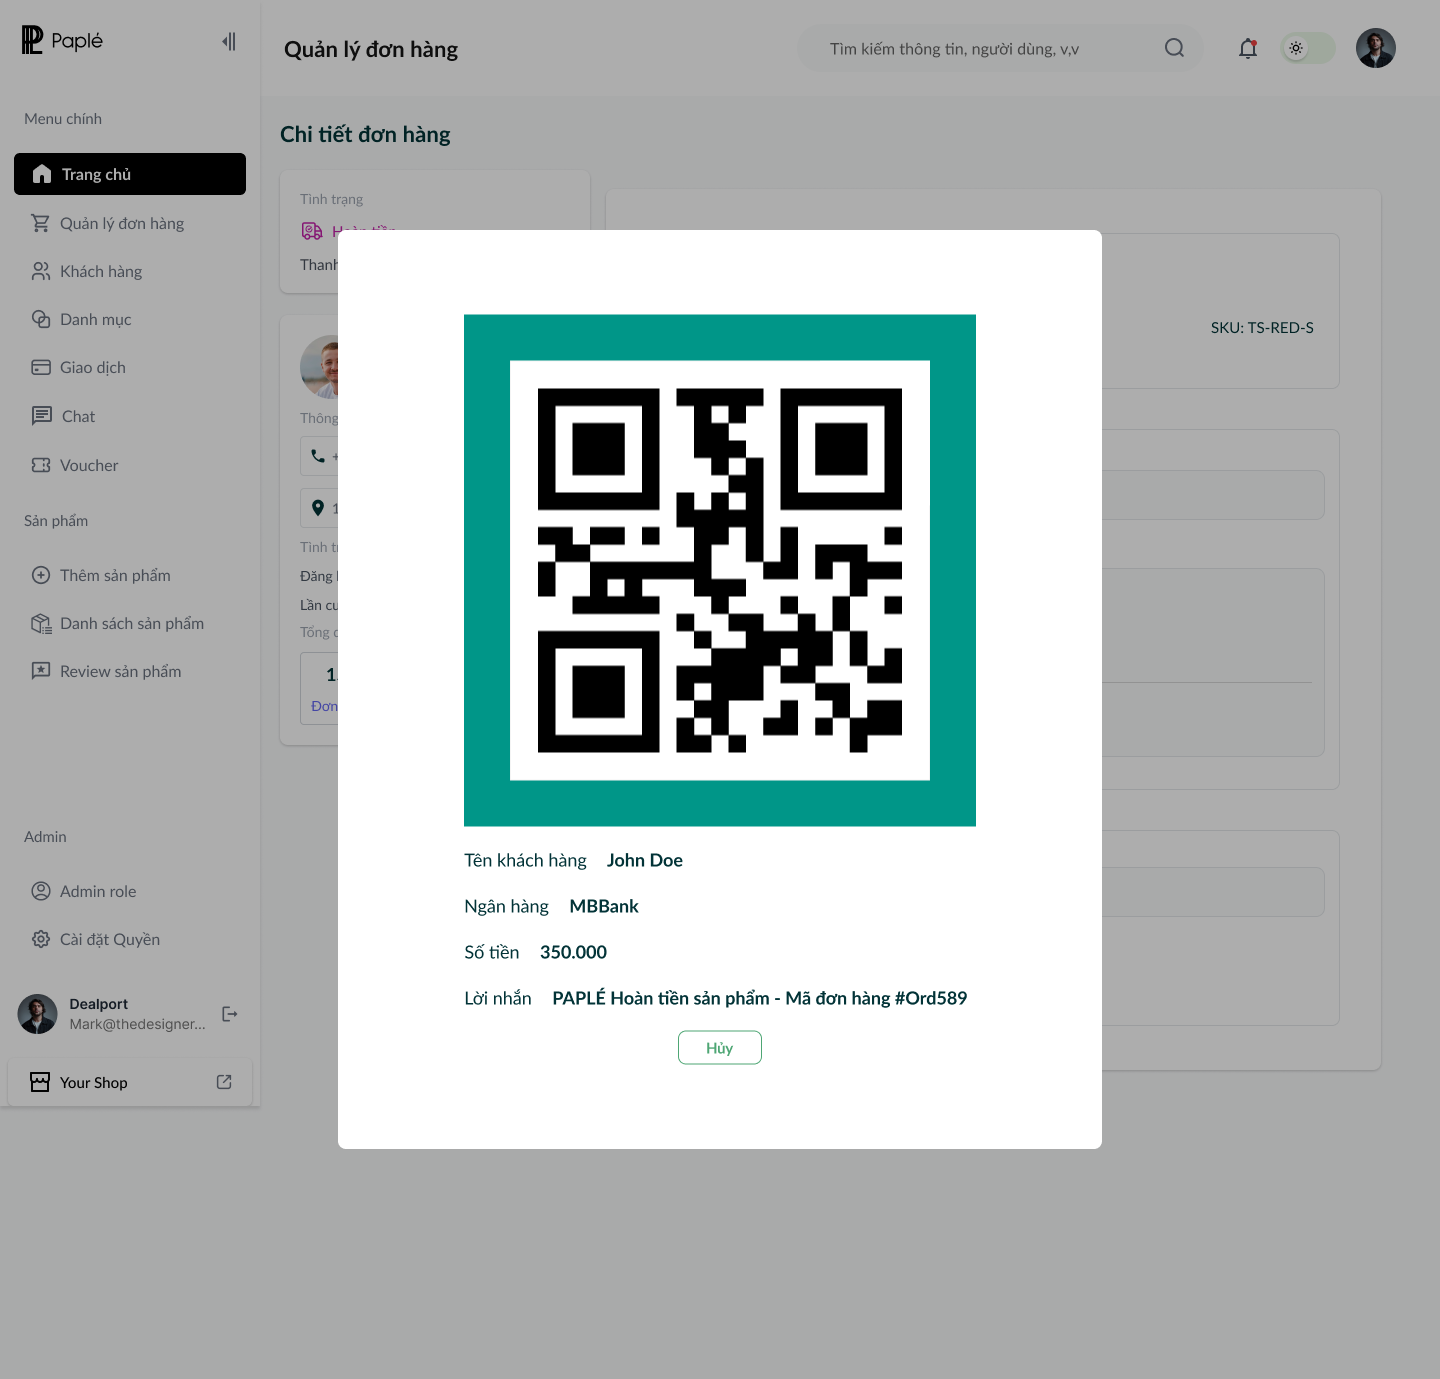
\includegraphics[width=1\textwidth]{Images/MockUp/Admin/Returned Order 1A.png}
                        \vspace{0.5cm}
                        \caption{Modal xác nhận hoàn tiền}
                        \label{fig: Modal xác nhận hoàn tiền}
                    \end{figure}
              \item \textbf{Từ chối yêu cầu:} Khi từ chối yêu cầu, hệ thống sẽ mở modal yêu cầu nhập lý do từ chối để thông báo cho khách hàng.
                    \begin{figure}[H]
                        \centering
                        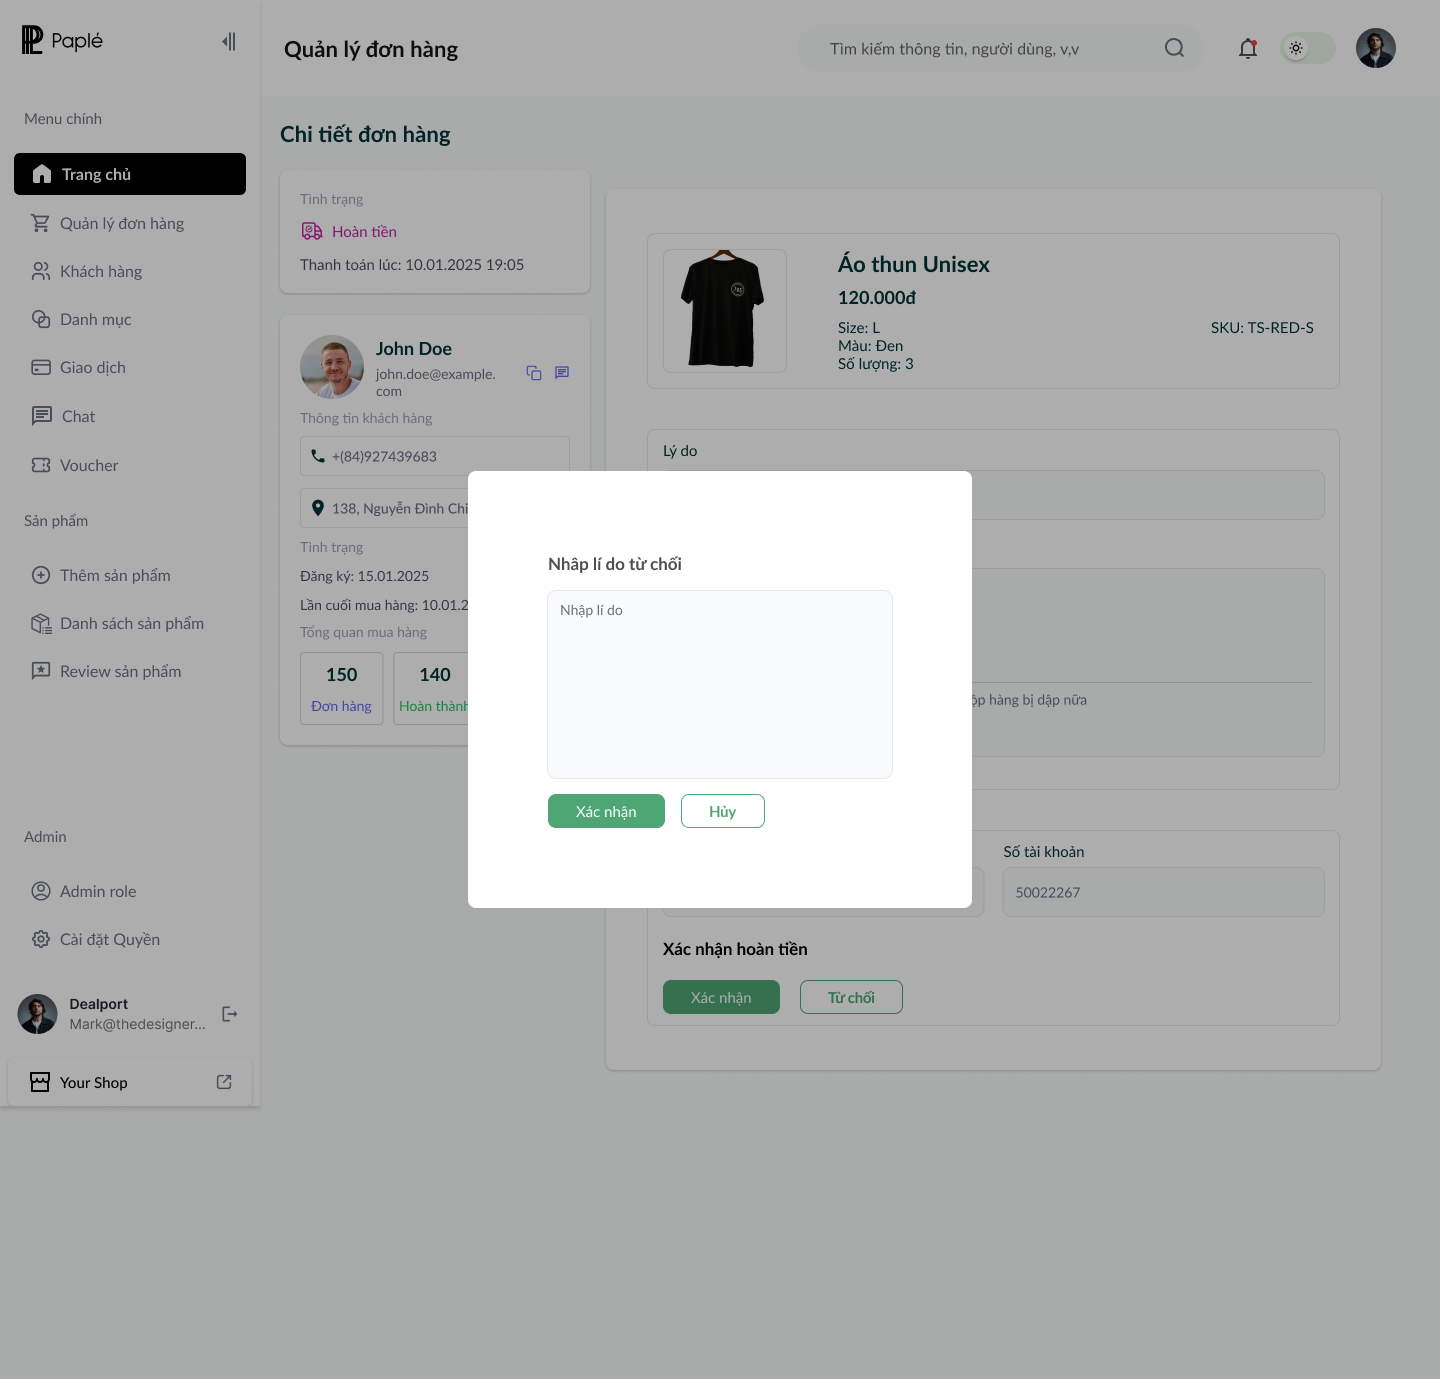
\includegraphics[width=1\textwidth]{Images/MockUp/Admin/Returned Order 1B.png}
                        \vspace{0.5cm}
                        \caption{Modal nhập lý do từ chối}
                        \label{fig: Modal nhập lý do từ chối}
                    \end{figure}
          \end{itemize}
\end{enumerate}

\subsubsubsection {Quản lý khách hàng}
\begin{figure}[H]
    \centering
    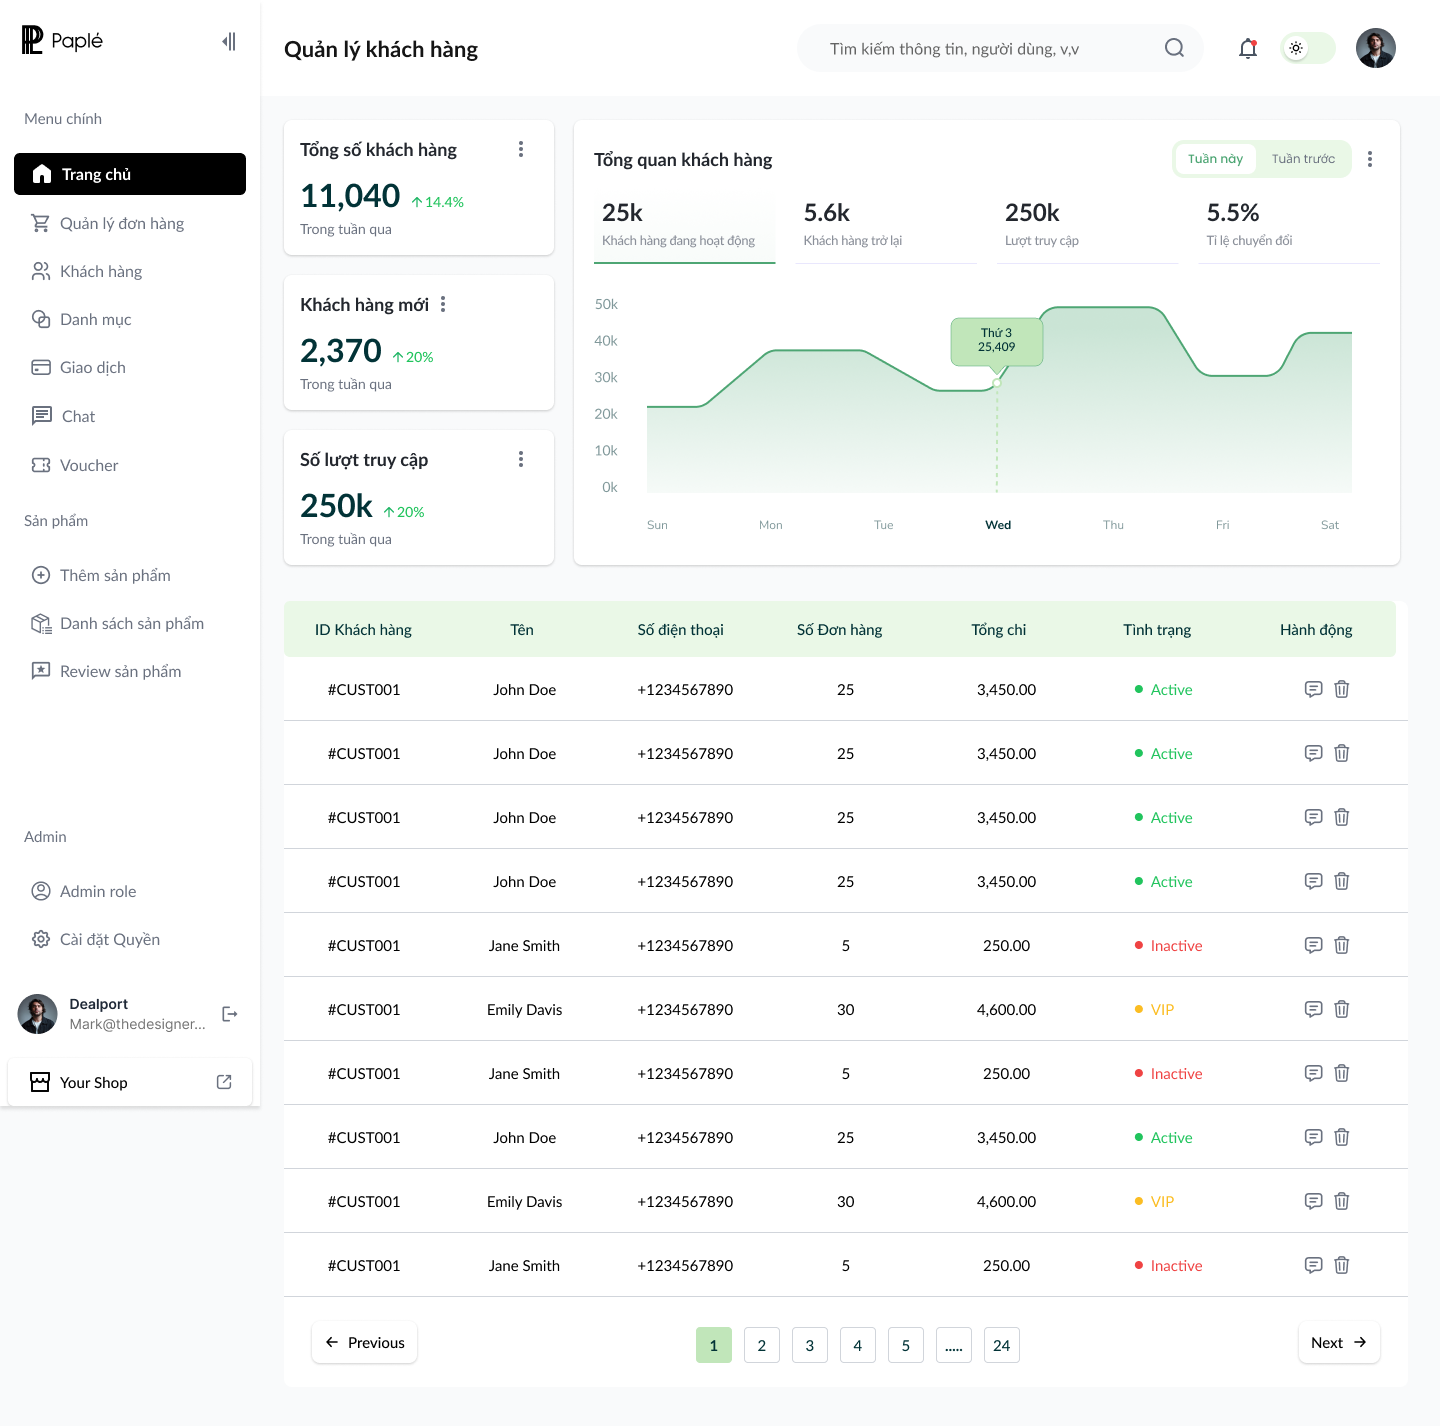
\includegraphics[width=1\textwidth]{Images/MockUp/Admin/Customer.png}
    \vspace{0.5cm}
    \caption{Giao diện quản lý khách hàng}
    \label{fig: Giao diện quản lý khách hàng}
\end{figure}
\noindent\textbf{Các thao tác chính:} Xem danh sách khách hàng, tìm kiếm và lọc khách hàng, xem chi tiết tài khoản, quản lý quyền truy cập, và theo dõi hoạt động khách hàng.

\subsubsubsection {Chi tiết khách hàng}
\begin{figure}[H]
    \centering
    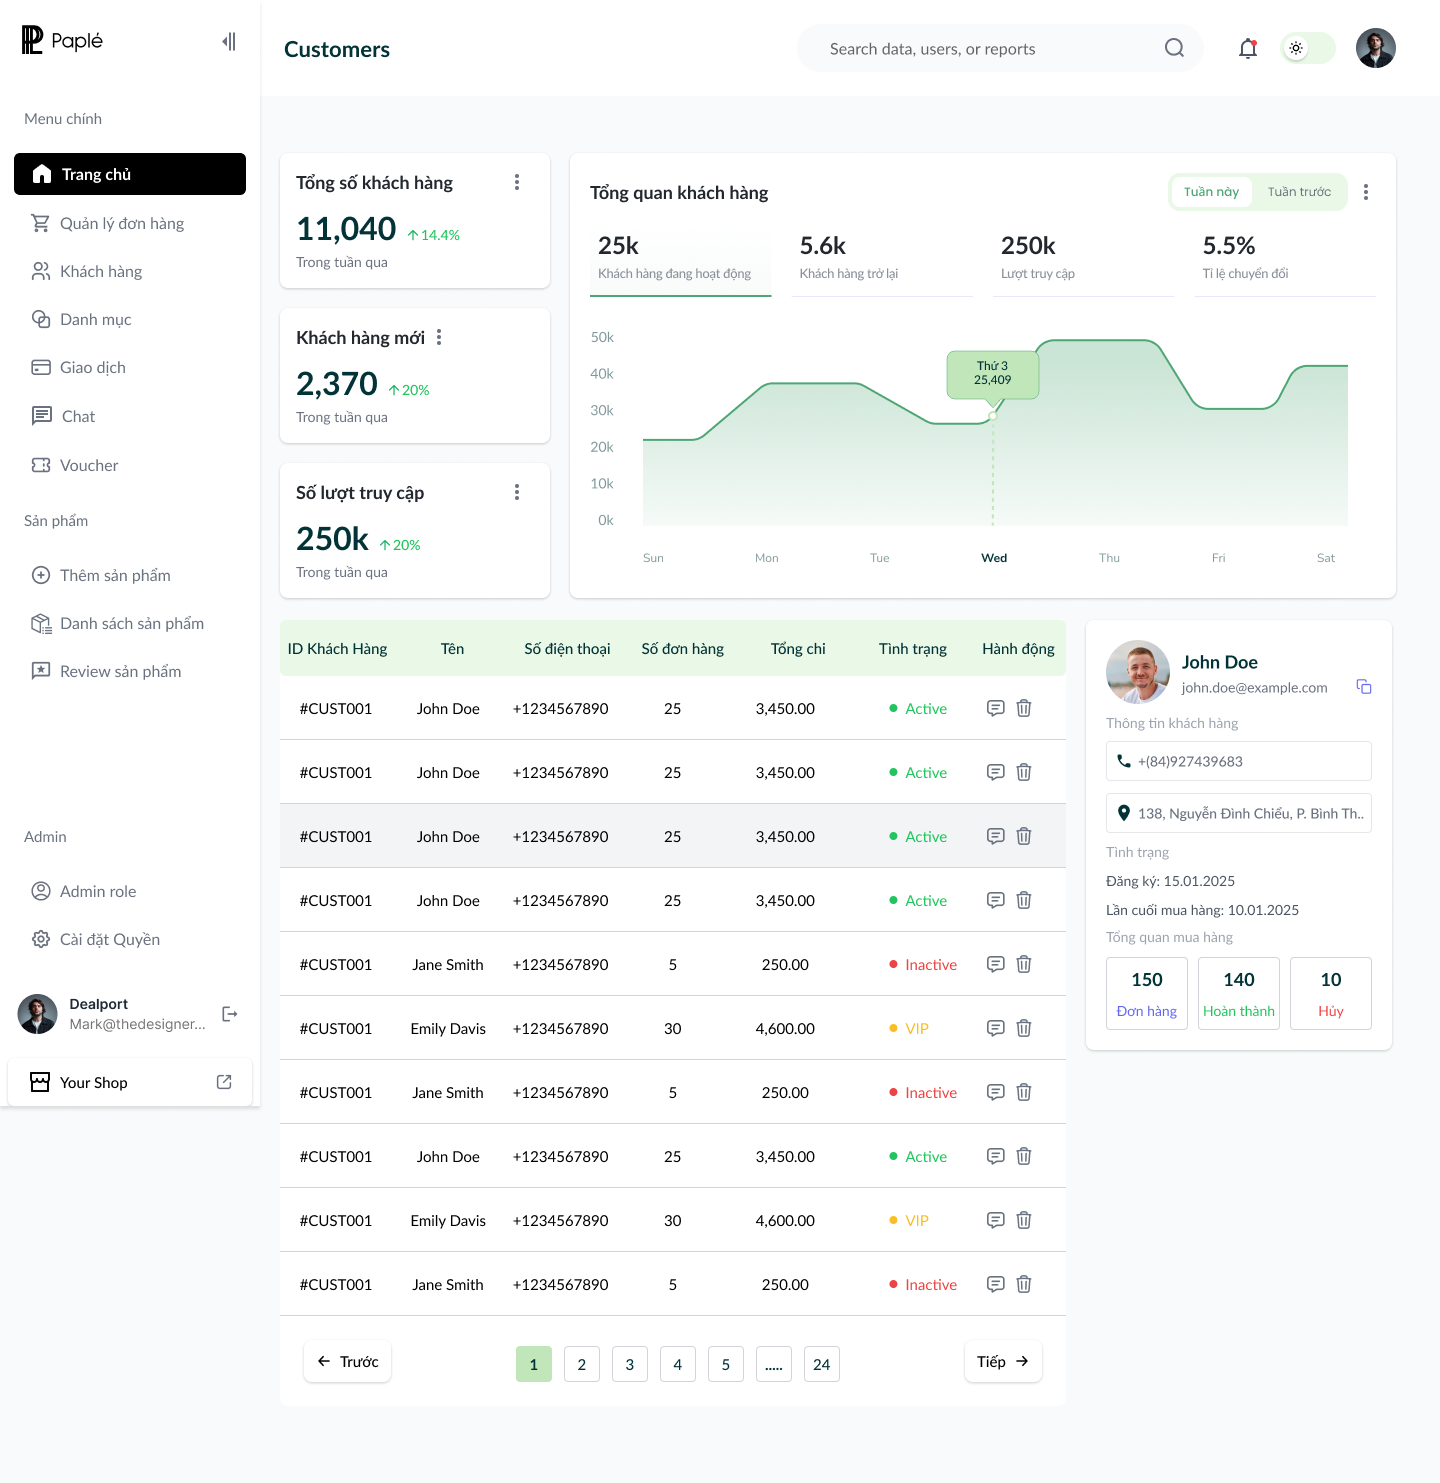
\includegraphics[width=1\textwidth]{Images/MockUp/Admin/Customer Details.png}
    \vspace{0.5cm}
    \caption{Giao diện chi tiết khách hàng}
    \label{fig: Giao diện chi tiết khách hàng}
\end{figure}
\noindent\textbf{Mô tả:} Hiển thị thông tin tài khoản khách hàng: tên, email, số điện thoại, địa chỉ mặc định, lịch sử đơn hàng.

\subsubsubsection {Quản lý voucher}
\begin{figure}[H]
    \centering
    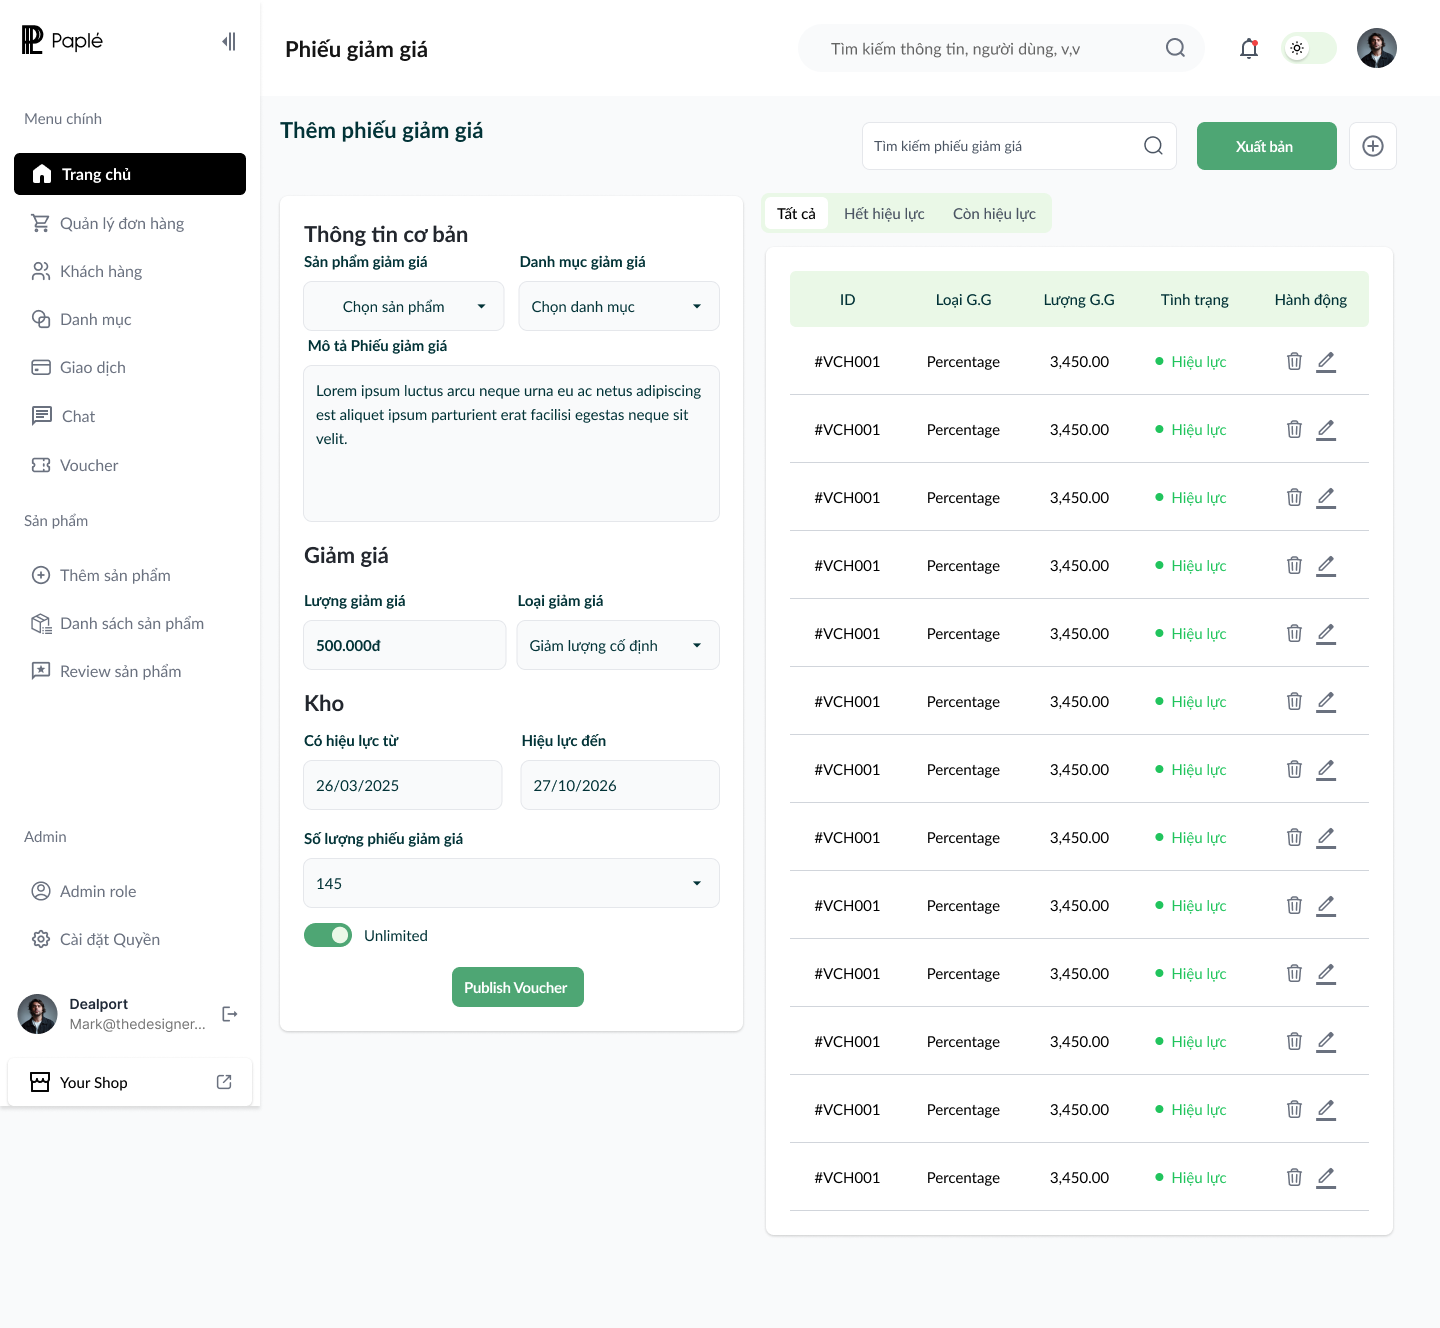
\includegraphics[width=1\textwidth]{Images/MockUp/Admin/Add Voucher.png}
    \vspace{0.5cm}
    \caption{Giao diện quản lý voucher}
    \label{fig: Giao diện quản lý voucher}
\end{figure}
\noindent\textbf{Các thao tác chính:} Xem danh sách voucher đã tạo, lọc theo trạng thái, xem chi tiết sử dụng, và quản lý hạn mức voucher.

\subsubsubsection {Quản lý danh mục}
\begin{figure}[H]
    \centering
    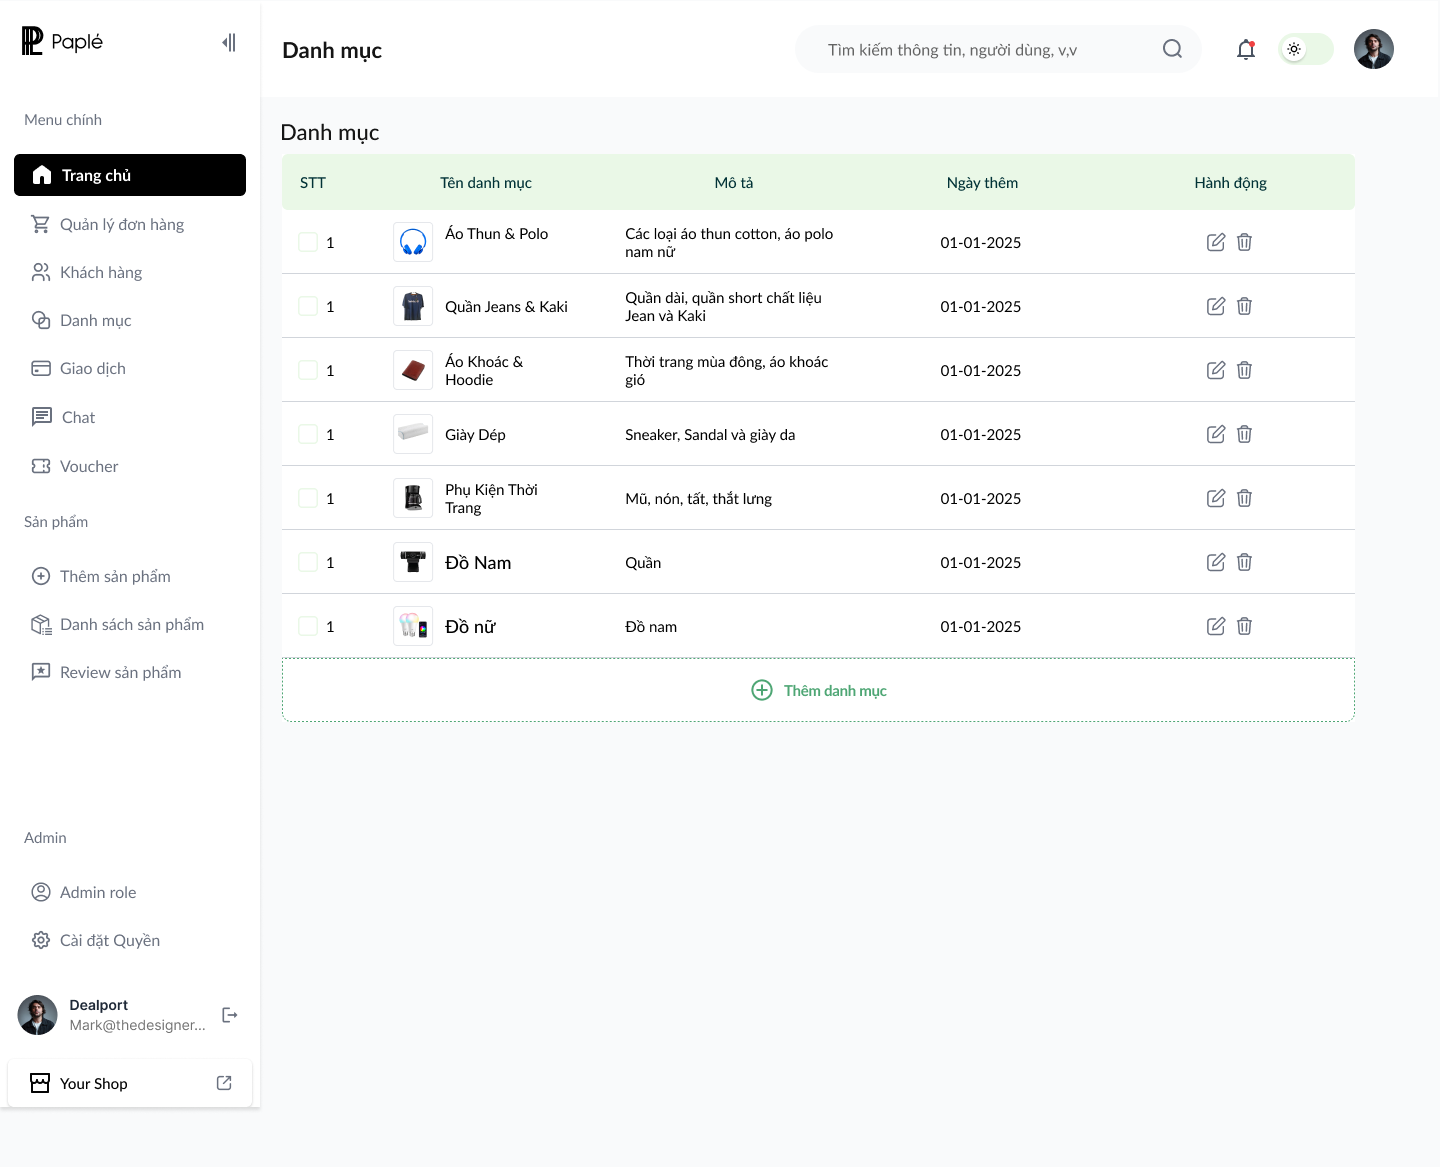
\includegraphics[width=1\textwidth]{Images/MockUp/Admin/Categories.png}
    \vspace{0.5cm}
    \caption{Giao diện quản lý danh mục}
    \label{fig: Giao diện quản lý danh mục}
\end{figure}
\noindent\textbf{Các thao tác chính:} Xem danh sách danh mục sản phẩm, thêm danh mục mới, chỉnh sửa và xóa danh mục, sắp xếp danh mục.

\subsubsubsection {Quản lý giao dịch}
\begin{figure}[H]
    \centering
    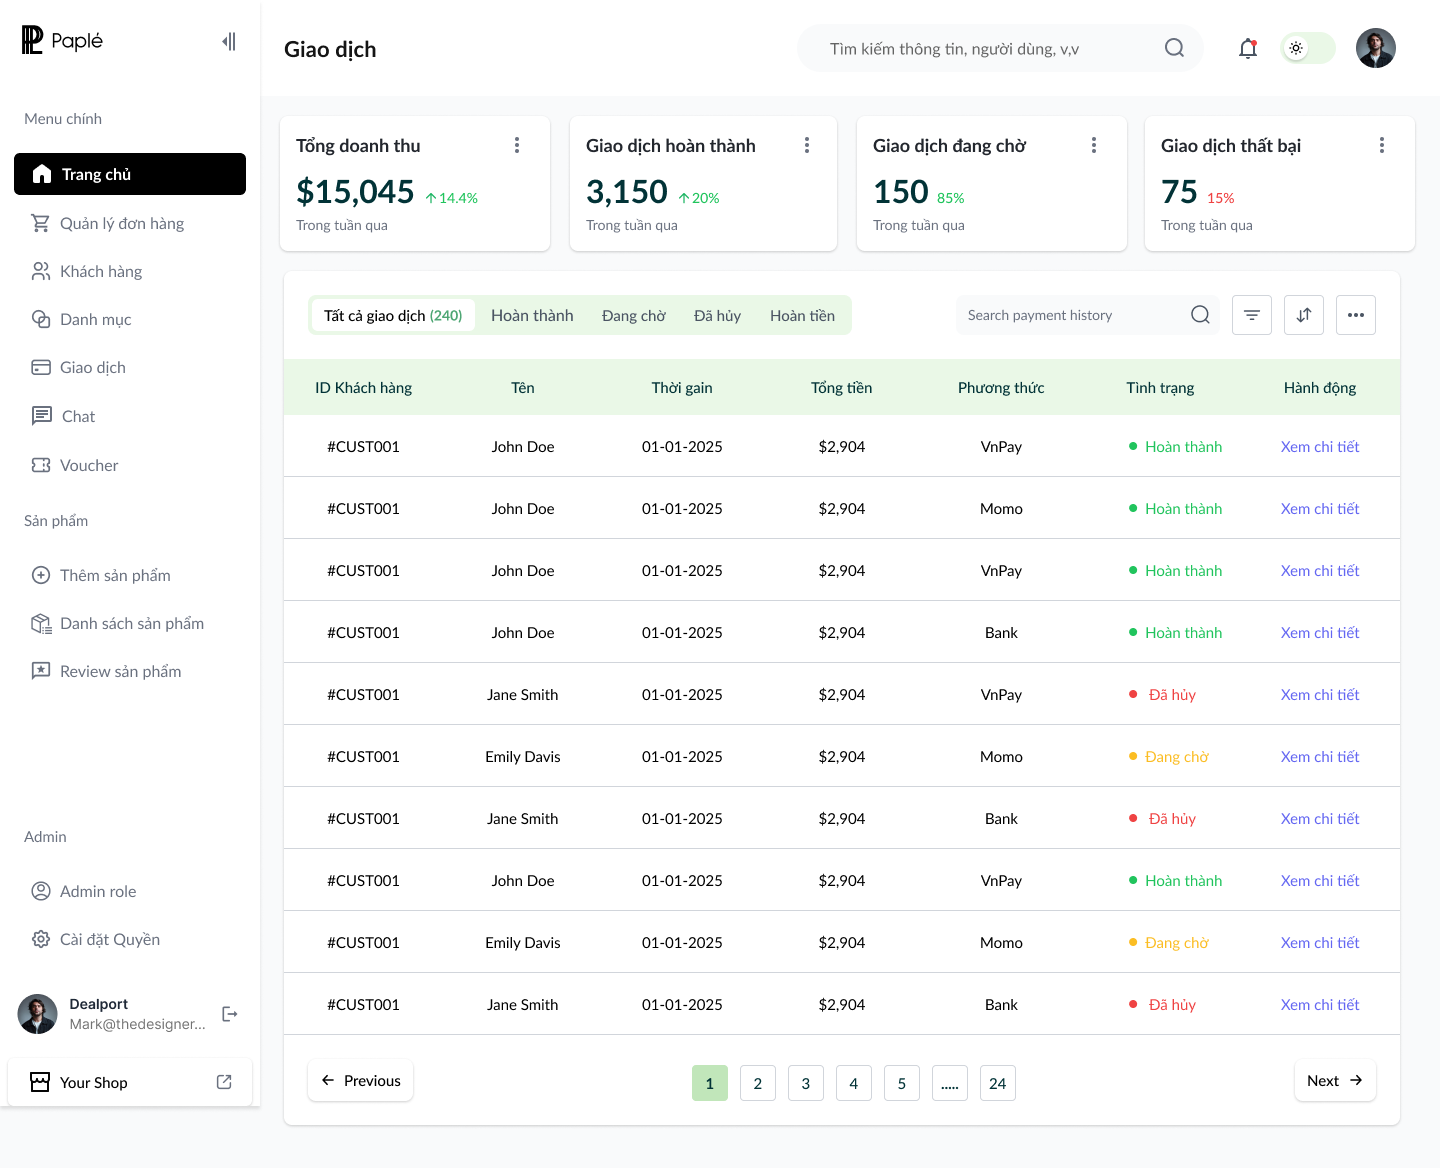
\includegraphics[width=1\textwidth]{Images/MockUp/Admin/Transaction.png}
    \vspace{0.5cm}
    \caption{Giao diện quản lý giao dịch}
    \label{fig: Giao diện quản lý giao dịch}
\end{figure}
\noindent\textbf{Các thao tác chính:} Xem lịch sử giao dịch, lọc theo loại giao dịch, xem chi tiết thanh toán, và kiểm tra xác minh thanh toán.

\subsubsubsection {Chi tiết giao dịch}
\begin{figure}[H]
    \centering
    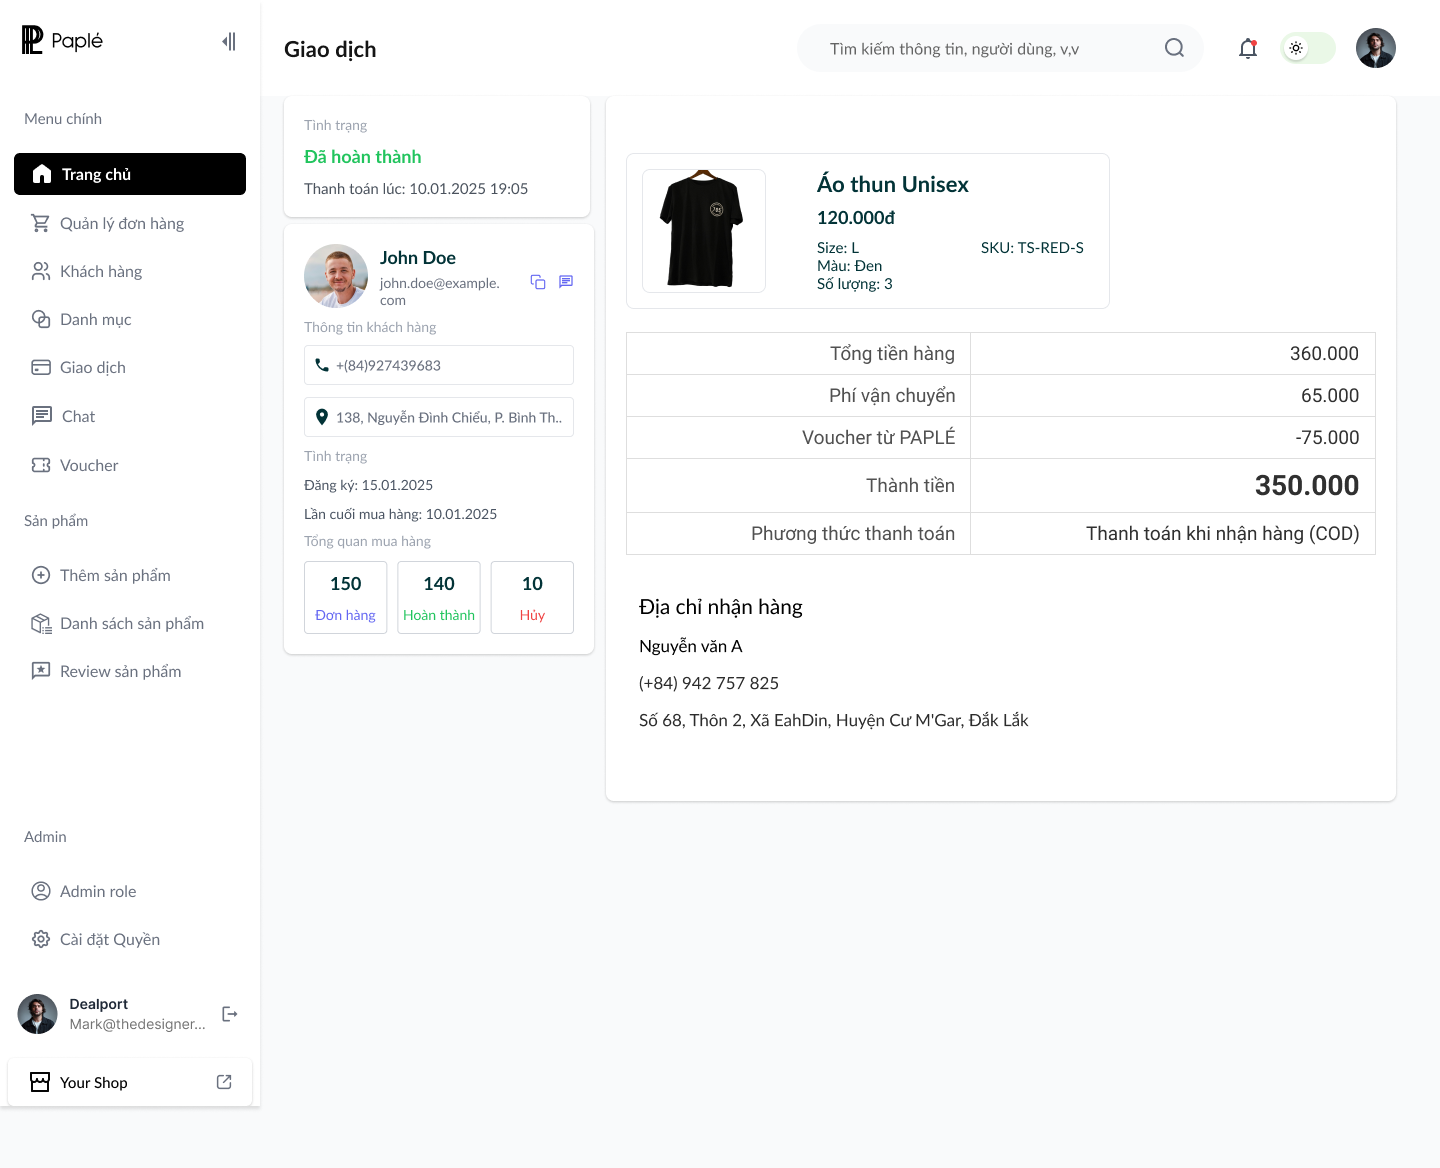
\includegraphics[width=1\textwidth]{Images/MockUp/Admin/Transaction Details.png}
    \vspace{0.5cm}
    \caption{Giao diện chi tiết giao dịch}
    \label{fig: Giao diện chi tiết giao dịch}
\end{figure}
\noindent\textbf{Mô tả:} Hiển thị thông tin thanh toán: đơn hàng liên quan, số tiền, phương thức (VNPay/COD), trạng thái, biên lai/hoá đơn, lịch sử đối soát. Hỗ trợ xác minh, xuất báo cáo, và xử lý hoàn tiền khi cần.

\subsubsubsection {Chat hỗ trợ}
\begin{figure}[H]
    \centering
    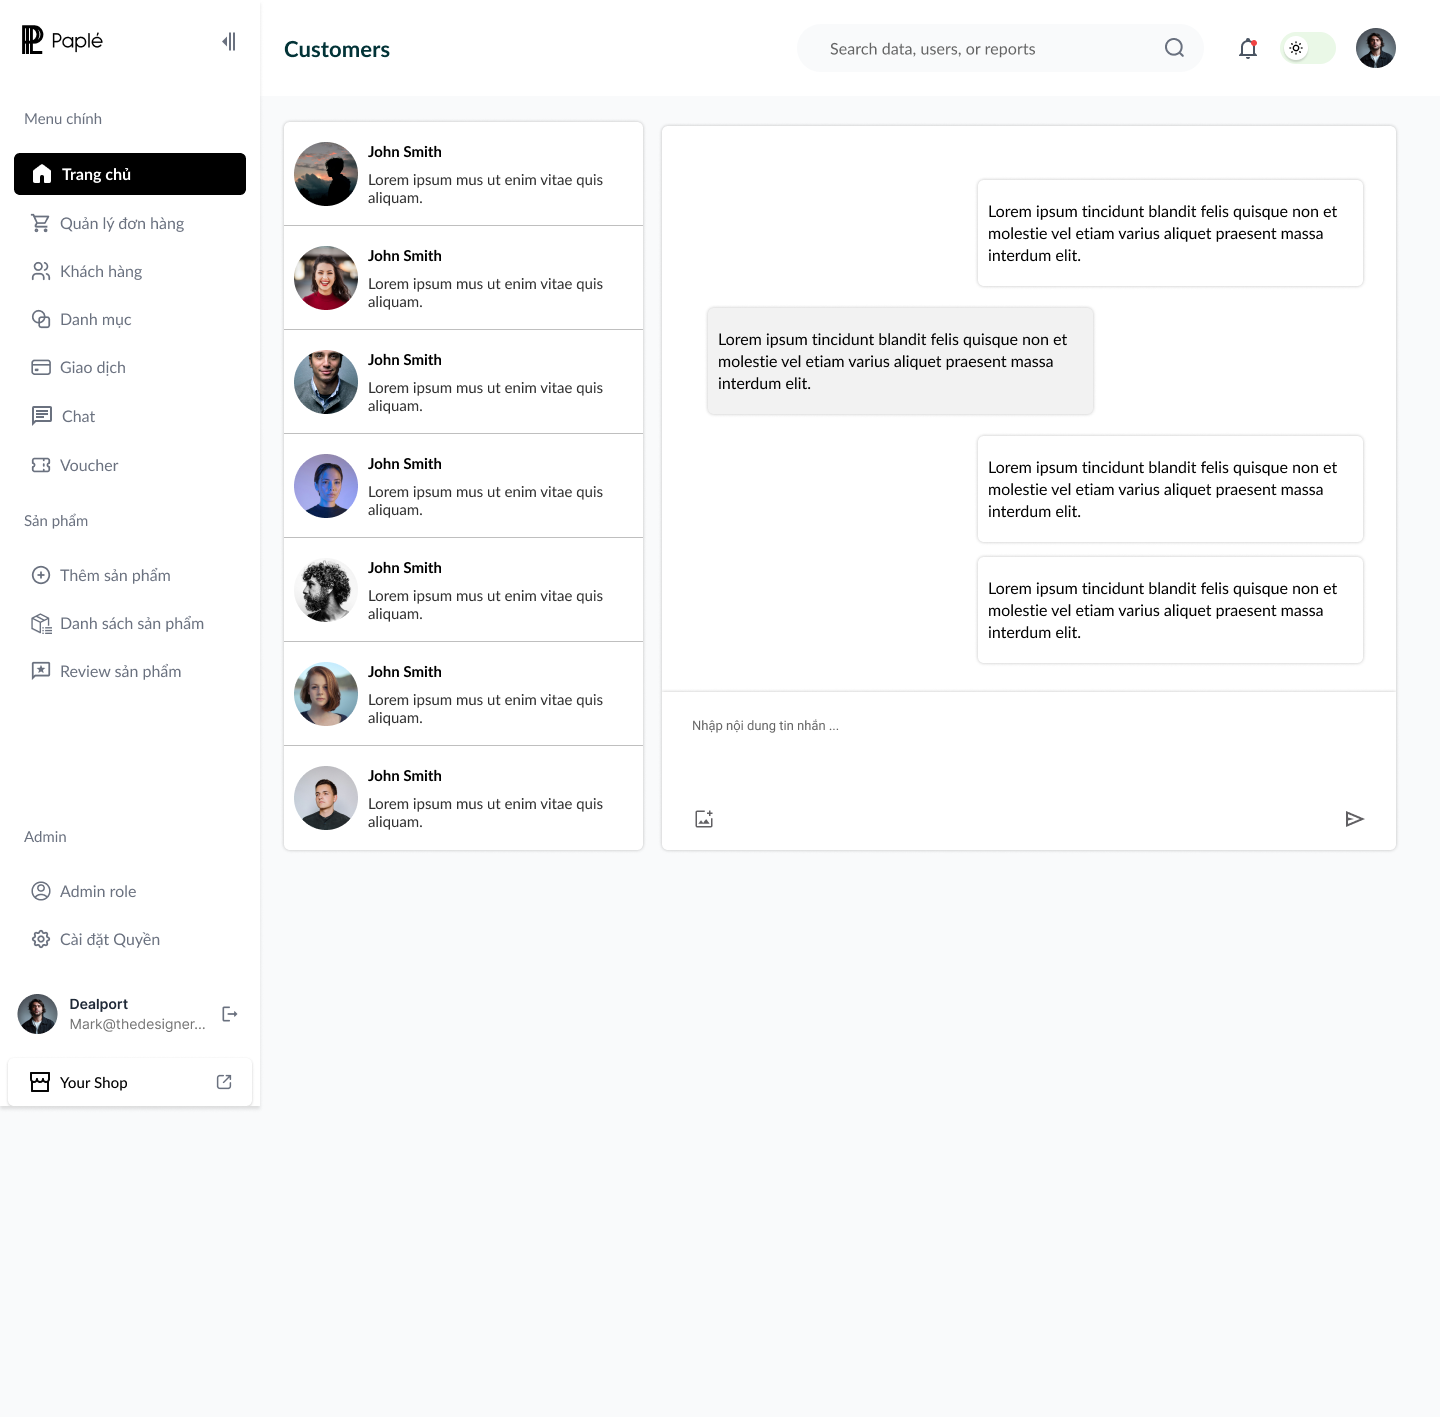
\includegraphics[width=1\textwidth]{Images/MockUp/Admin/Chat.png}
    \vspace{0.5cm}
    \caption{Giao diện chat hỗ trợ}
    \label{fig: Giao diện chat hỗ trợ}
\end{figure}
\noindent\textbf{Các thao tác chính:} Xem danh sách cuộc trò chuyện với khách hàng, trả lời tin nhắn, gửi hình ảnh hoặc tệp, và quản lý các yêu cầu hỗ trợ.

\subsubsubsection {Thêm/Chỉnh sửa sản phẩm}
\begin{figure}[H]
    \centering
    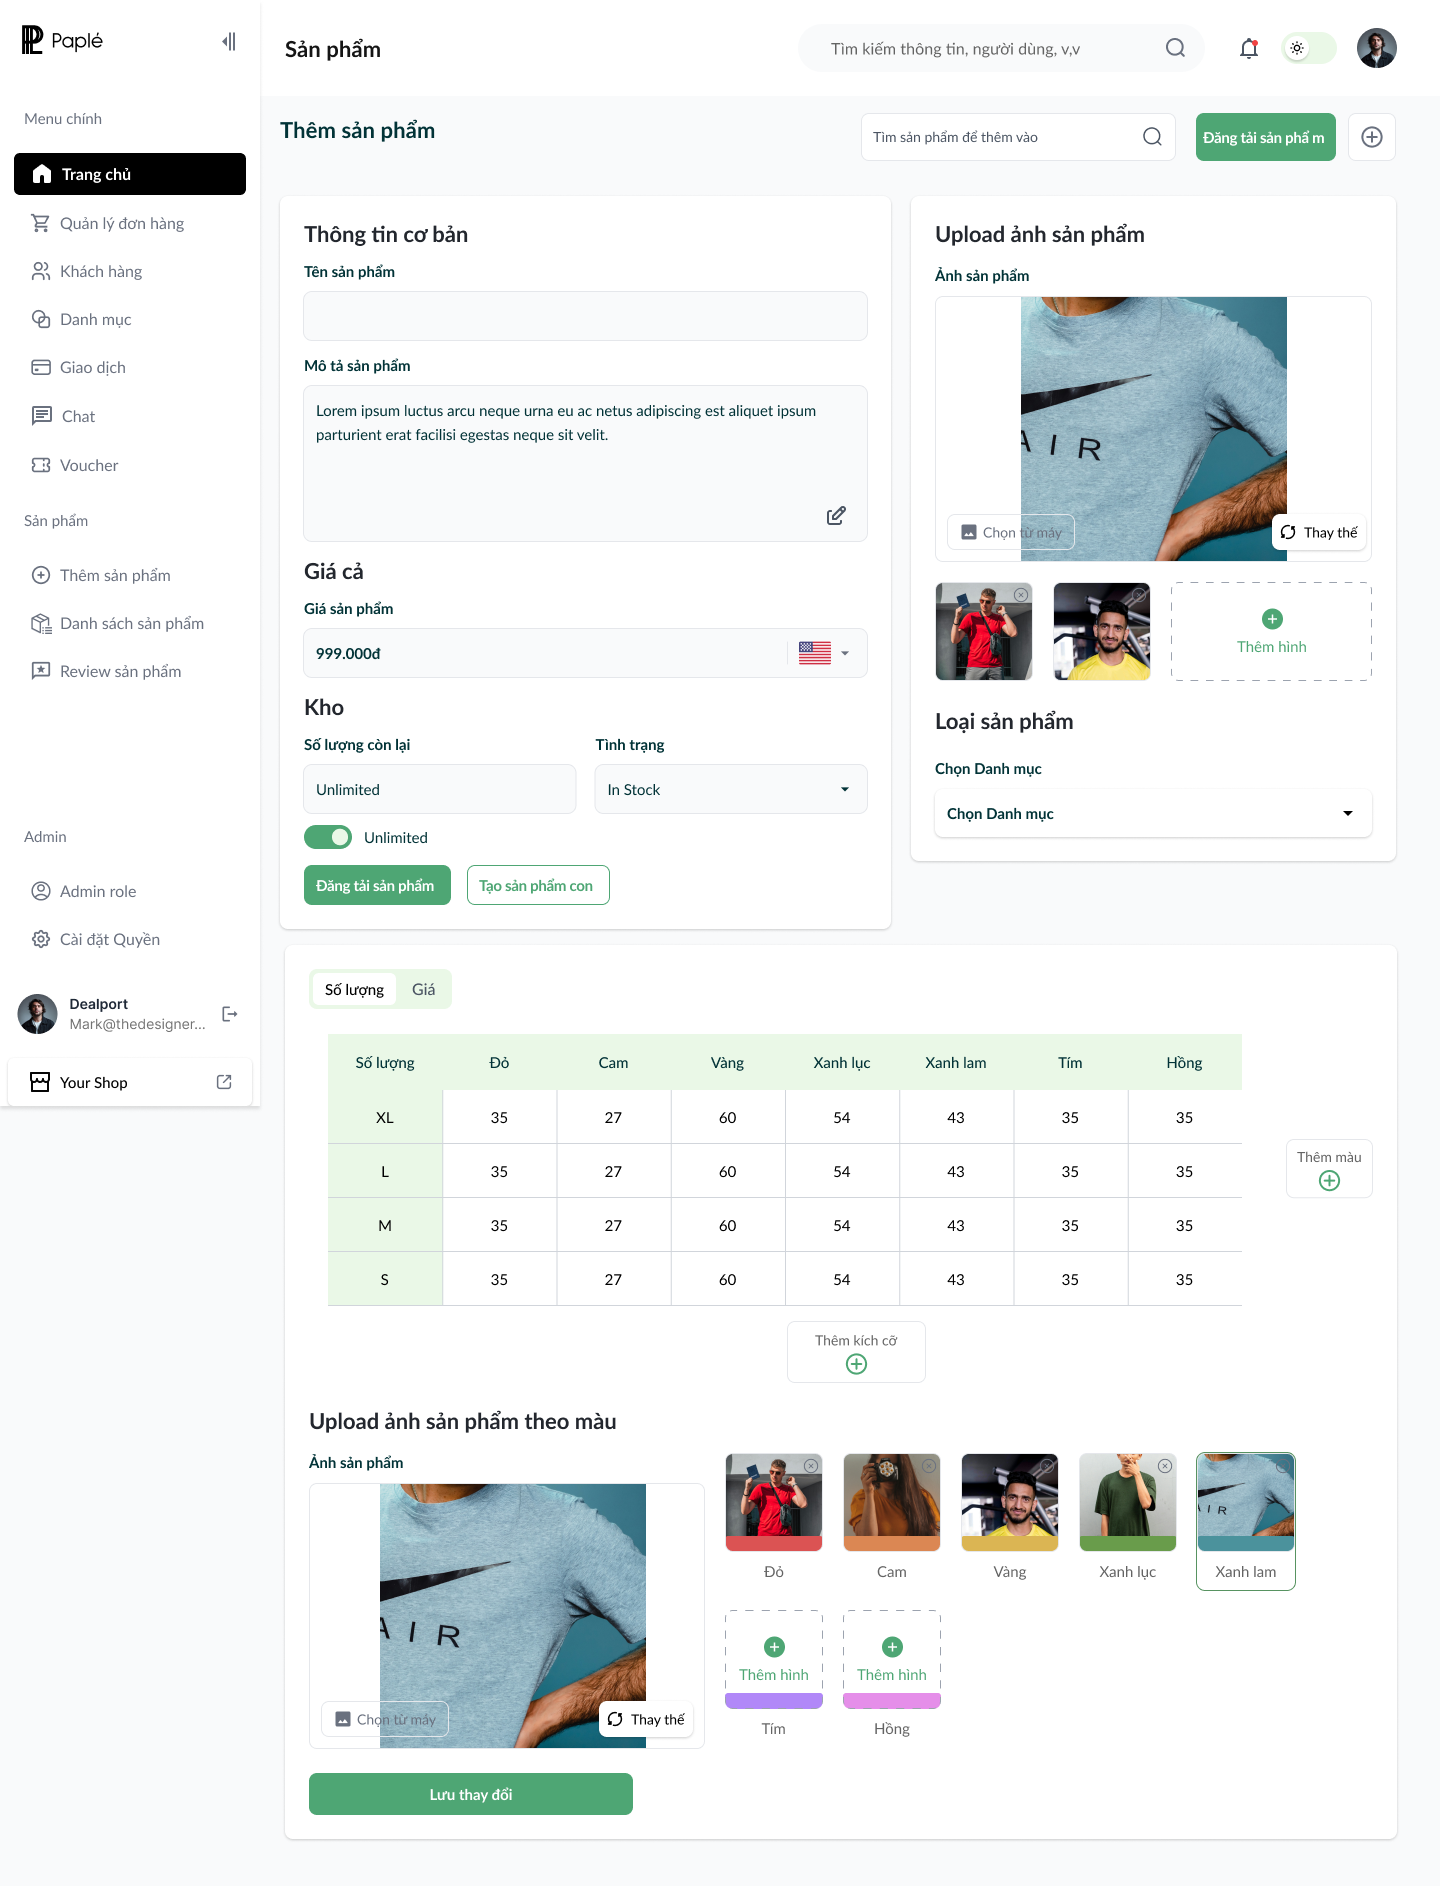
\includegraphics[width=1\textwidth]{Images/MockUp/Admin/Add+edit Product.png}
    \vspace{0.5cm}
    \caption{Giao diện thêm/chỉnh sửa sản phẩm}
    \label{fig: Giao diện thêm/chỉnh sửa sản phẩm}
\end{figure}
\noindent\textbf{Các thao tác chính:} Nhập thông tin cơ bản của sản phẩm bao gồm tên sản phẩm, giá bán, mô tả chi tiết sản phẩm với trình soạn thảo văn bản định dạng. Chọn danh mục sản phẩm từ danh sách có sẵn. Tải lên nhiều hình ảnh sản phẩm. Thiết lập các biến thể sản phẩm (product variants) với các thuộc tính như kích cỡ (S, M, L, XL), màu sắc, quản lý số lượng tồn kho  và giá cho từng biến thể.

\subsubsubsection {Danh sách sản phẩm}
\begin{figure}[H]
    \centering
    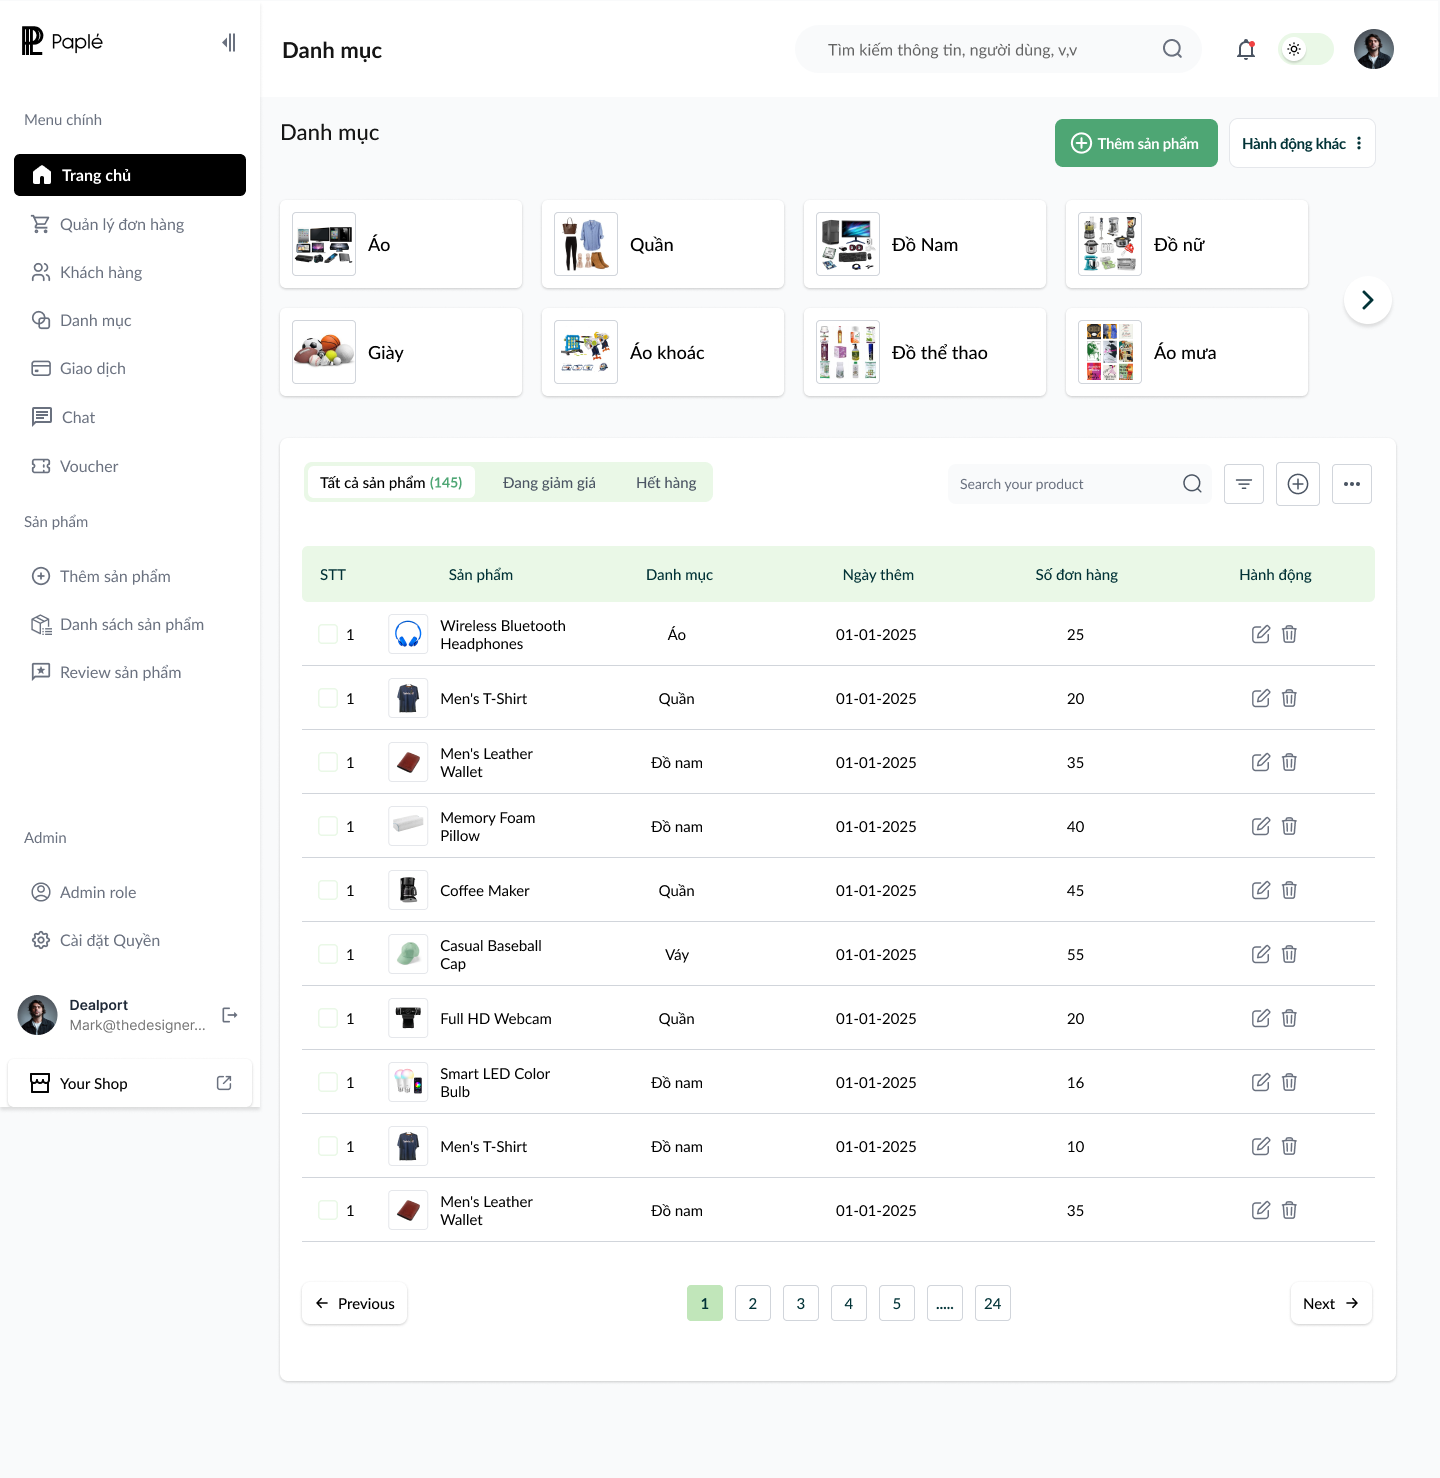
\includegraphics[width=1\textwidth]{Images/MockUp/Admin/Products.png}
    \vspace{0.5cm}
    \caption{Giao diện danh sách sản phẩm}
    \label{fig: Giao diện danh sách sản phẩm}
\end{figure}
\noindent\textbf{Mô tả:} Hiển thị bảng sản phẩm với các cột: hình ảnh, tên, danh mục, giá, tồn kho, trạng thái hiển thị. Cho phép tìm kiếm, lọc theo danh mục/trạng thái, sắp xếp theo giá/tồn kho, chỉnh sửa nhanh trạng thái, và truy cập chi tiết/chỉnh sửa.

\subsubsubsection {Phân quyền vai trò}
\begin{figure}[H]
    \centering
    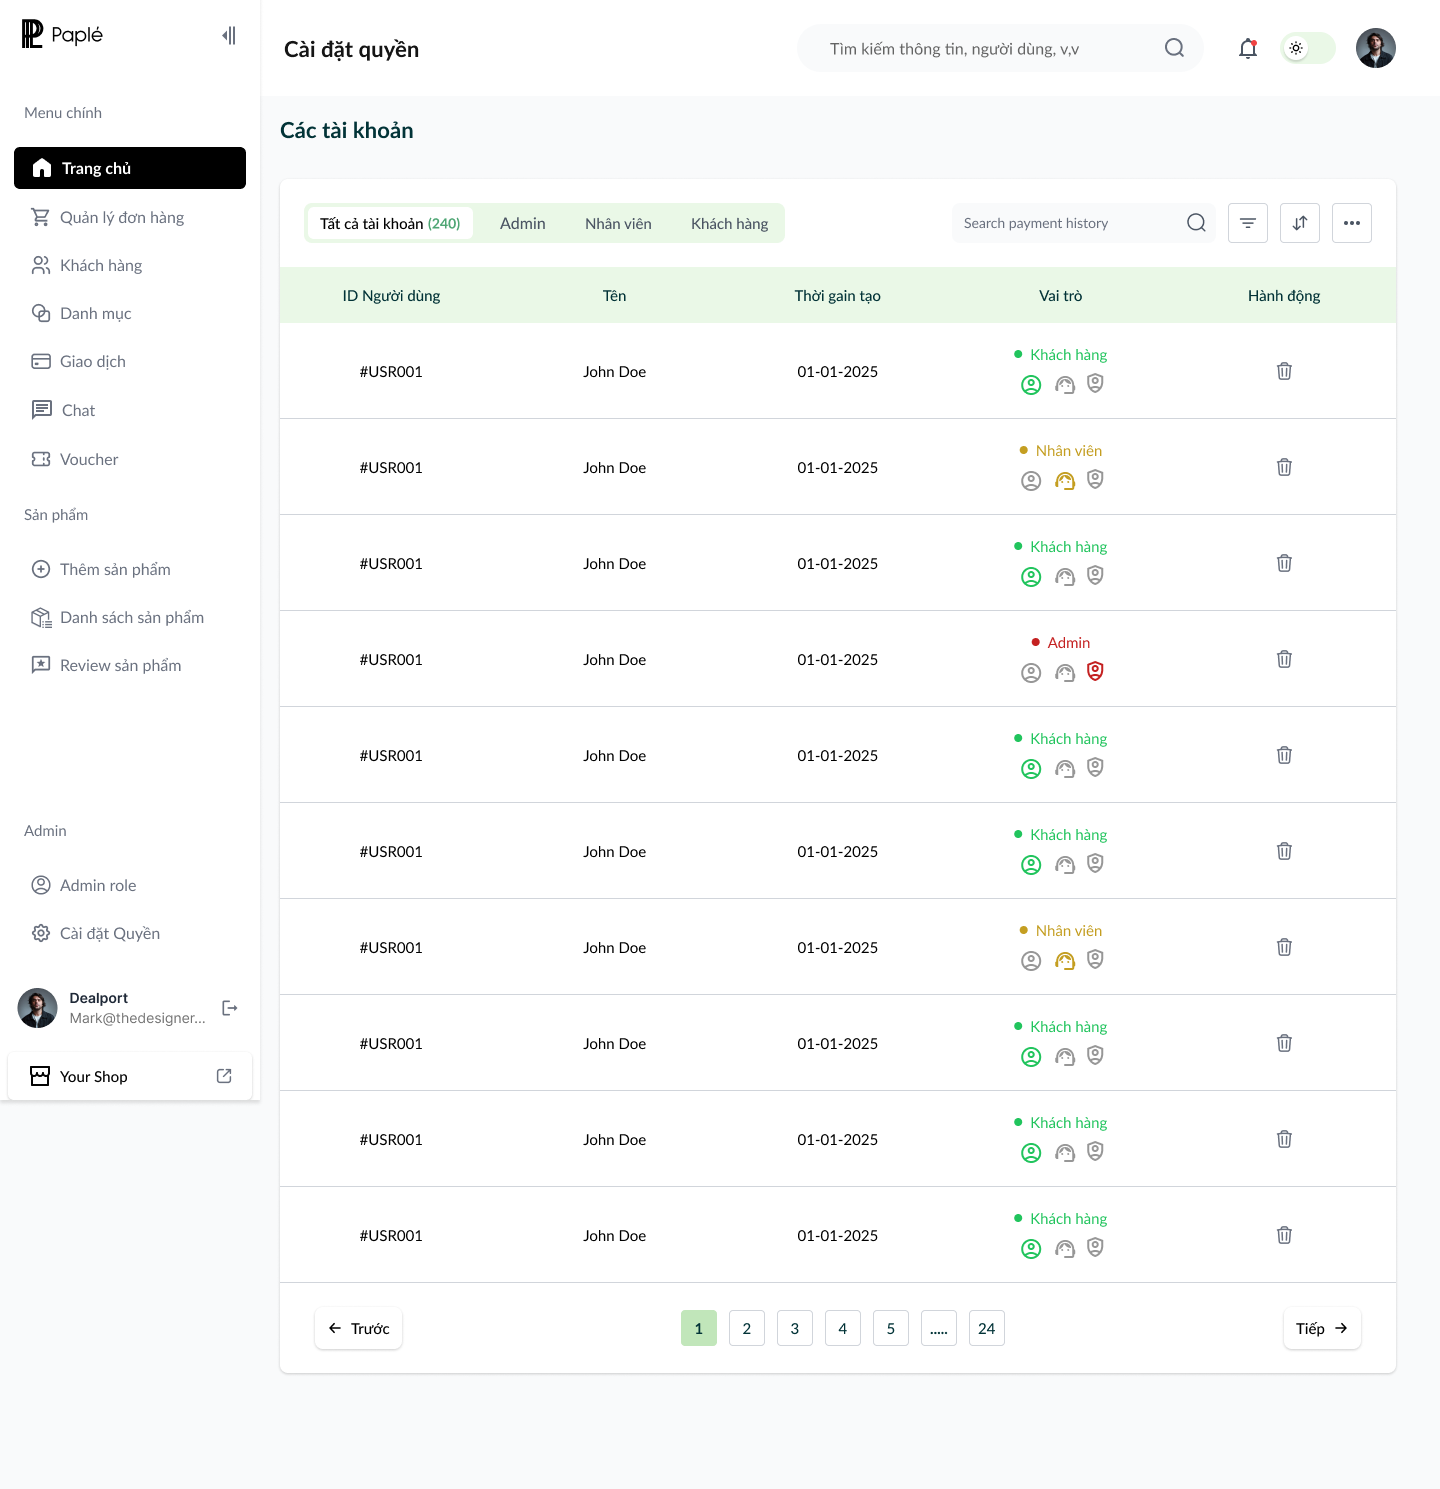
\includegraphics[width=1\textwidth]{Images/MockUp/Admin/Role Control.png}
    \vspace{0.5cm}
    \caption{Giao diện phân quyền vai trò}
    \label{fig: Giao diện phân quyền vai trò}
\end{figure}
\noindent\textbf{Mô tả:} Quản lý quyền truy cập theo vai trò (Admin, Staff). Cho phép gán vai trò cho người dùng.

\subsubsubsection {Quản lý trang cá nhân}
\begin{figure}[H]
    \centering
    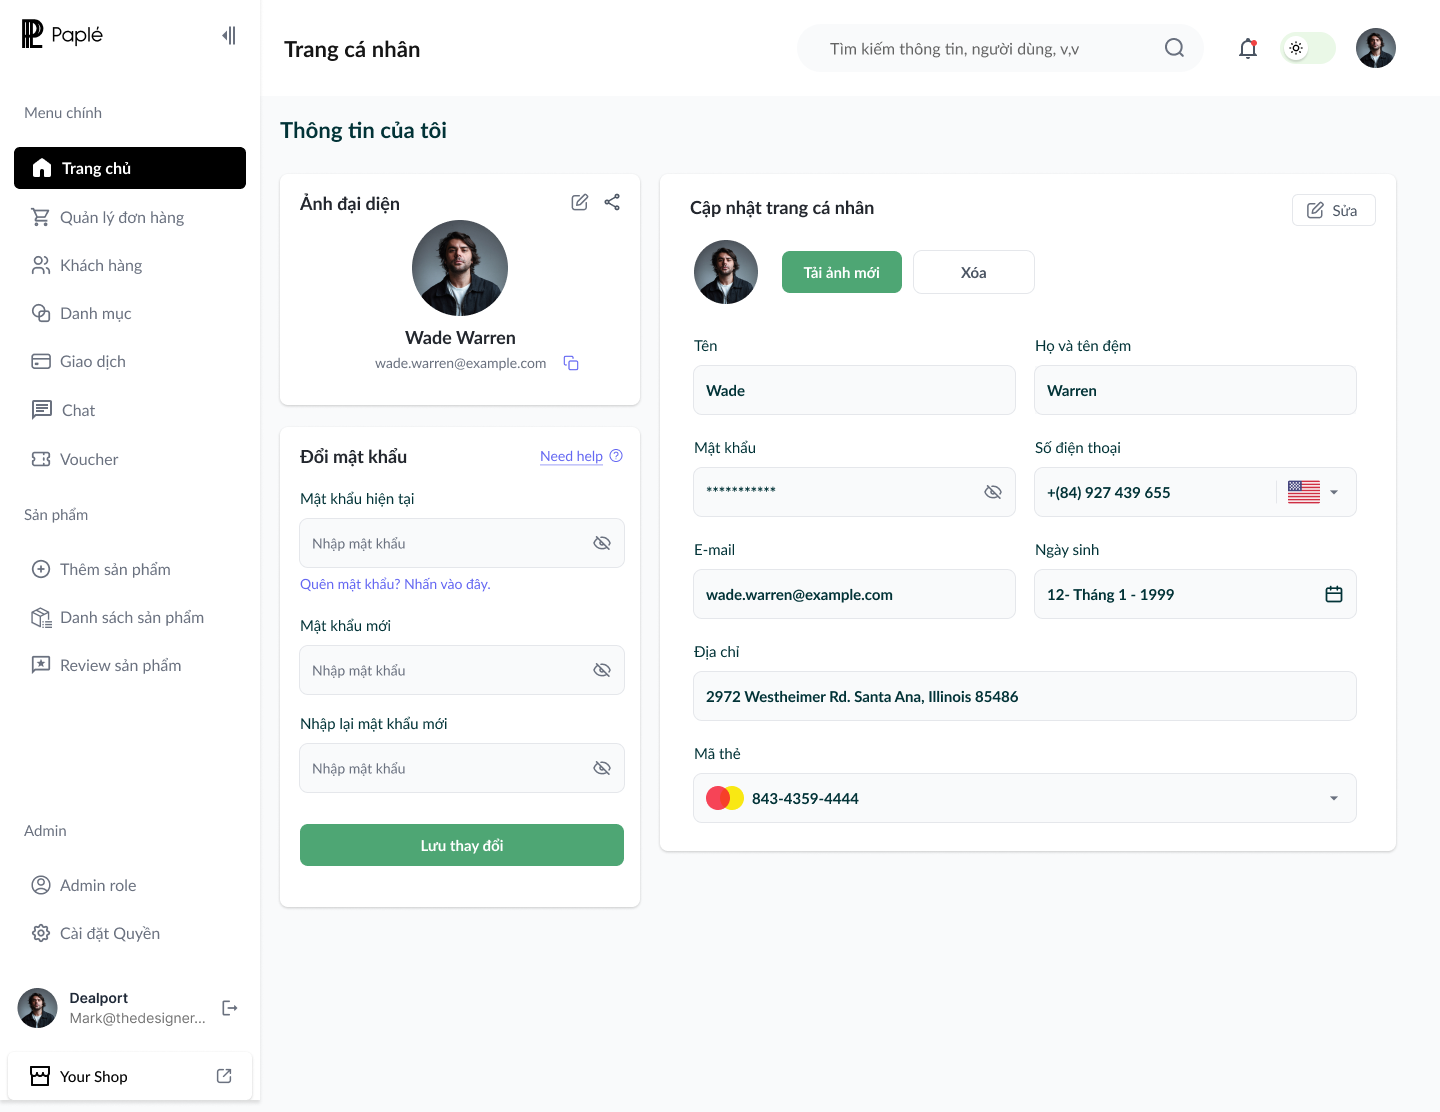
\includegraphics[width=1\textwidth]{Images/MockUp/Admin/Admin Role.png}
    \vspace{0.5cm}
    \caption{Giao diện quản lý trang cá nhân}
    \label{fig: Giao diện quản lý trang cá nhân}
\end{figure}
\noindent\textbf{Các thao tác chính:} Xem danh sách người dùng hệ thống, phân quyền và vai trò (admin, nhân viên), chỉnh sửa quyền truy cập, khóa tài khoản, và xem lịch sử hoạt động.

\subsubsection{Thiết kế giao diện cho nhân viên}

\subsubsubsection {Quản lý đơn hàng}
\begin{figure}[H]
    \centering
    
\includegraphics[width=1\textwidth]{Images/MockUp/Staff/Order Management.png}
    \vspace{0.5cm}
    \caption{Giao diện quản lý đơn hàng (Nhân viên)}
    \label{fig: Giao diện quản lý đơn hàng nhân viên}
\end{figure}
\noindent\textbf{Các thao tác chính:} Xem danh sách đơn hàng, lọc theo trạng thái, cập nhật trạng thái xử lý đơn hàng, xác nhận đơn hàng. Không có quyền tạo/sửa/xóa sản phẩm, voucher.

\subsubsubsection {Chi tiết đơn hàng}
\begin{figure}[H]
    \centering
    
\includegraphics[width=1\textwidth]{Images/MockUp/Staff/Order Detail.png}
    \vspace{0.5cm}
    \caption{Giao diện chi tiết đơn hàng (Nhân viên)}
    \label{fig: Giao diện chi tiết đơn hàng nhân viên}
\end{figure}
\noindent\textbf{Mô tả:} Hiển thị thông tin chi tiết đơn hàng: mã đơn, khách hàng, địa chỉ giao hàng, danh sách sản phẩm, tổng tiền. Cho phép cập nhật trạng thái đơn hàng, xem lịch sử xử lý.

\subsubsubsection {Danh sách sản phẩm}
\begin{figure}[H]
    \centering
    
\includegraphics[width=1\textwidth]{Images/MockUp/Staff/Products.png}
    \vspace{0.5cm}
    \caption{Giao diện danh sách sản phẩm (Nhân viên)}
    \label{fig: Giao diện danh sách sản phẩm nhân viên}
\end{figure}
\noindent\textbf{Mô tả:} Hiển thị danh sách sản phẩm với thông tin: tên,giá, tồn kho, trạng thái. Nhân viên chỉ có quyền xem (read-only) để tra cứu thông tin sản phẩm phục vụ tư vấn khách hàng. Không có quyền thêm, sửa, xóa sản phẩm hay thay đổi giá.

\subsubsubsection {Chi tiết sản phẩm}
\begin{figure}[H]
    \centering
    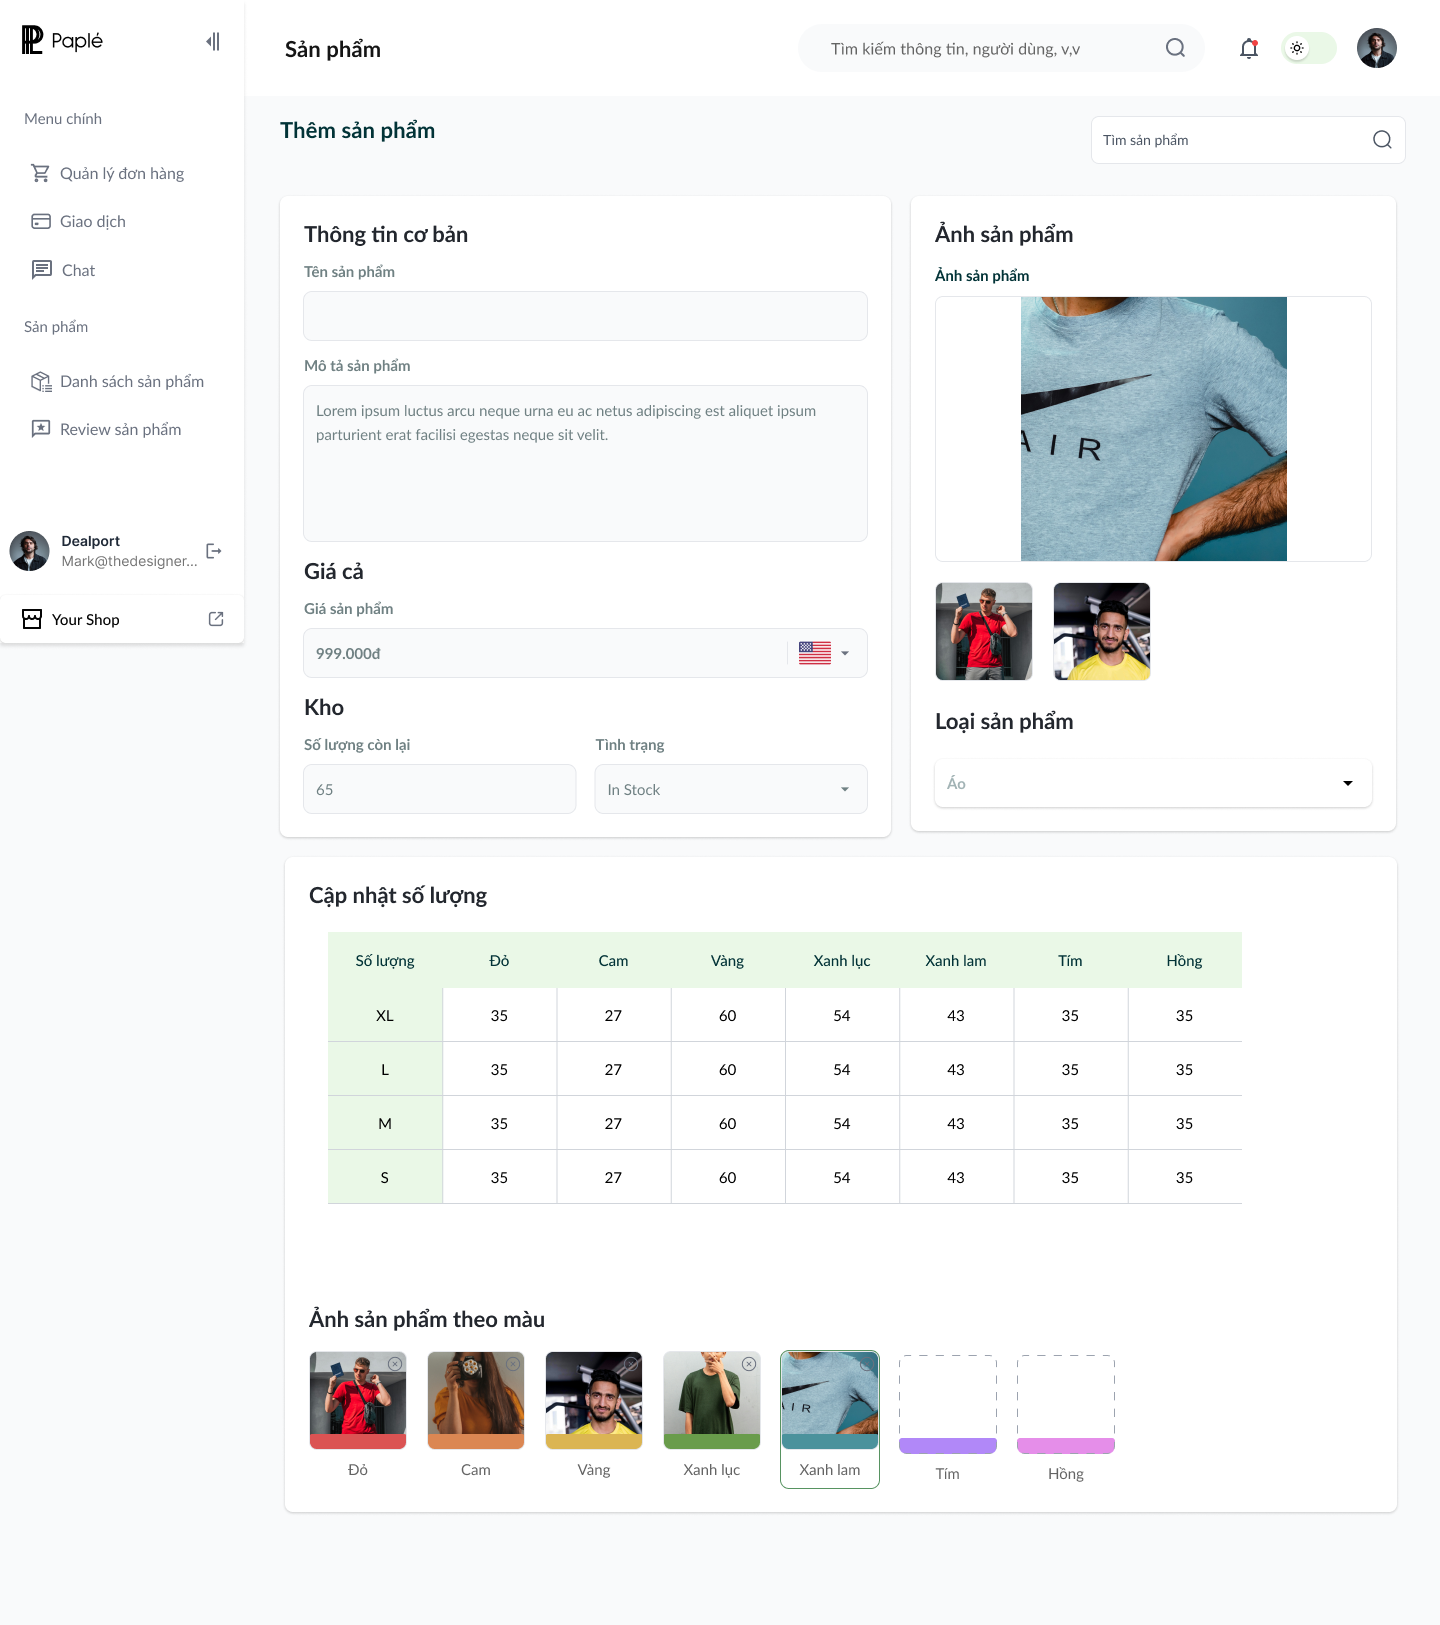
\includegraphics[width=1\textwidth]{Images/MockUp/Staff/Product Detail.png}
    \vspace{0.5cm}
    \caption{Giao diện chi tiết sản phẩm (Nhân viên)}
    \label{fig: Giao diện chi tiết sản phẩm nhân viên}
\end{figure}
\noindent\textbf{Mô tả:} Hiển thị thông tin đầy đủ về sản phẩm: tên, mô tả, giá, các biến thể (màu sắc, kích cỡ), số lượng tồn kho từng biến thể, hình ảnh sản phẩm. Chế độ chỉ xem, không cho phép chỉnh sửa bất kỳ thông tin nào trừ tồn kho.

\subsubsubsection {Quản lý giao dịch}
\begin{figure}[H]
    \centering
    
\includegraphics[width=1\textwidth]{Images/MockUp/Staff/Transaction.png}
    \vspace{0.5cm}
    \caption{Giao diện quản lý giao dịch (Nhân viên)}
    \label{fig: Giao diện quản lý giao dịch nhân viên}
\end{figure}
\noindent\textbf{Các thao tác chính:} Xem lịch sử giao dịch thanh toán liên quan đến đơn hàng, lọc theo trạng thái, xác minh thanh toán.

\subsubsubsection {Chi tiết giao dịch}
\begin{figure}[H]
    \centering
    
\includegraphics[width=1\textwidth]{Images/MockUp/Staff/Transaction Details.png}
    \vspace{0.5cm}
    \caption{Giao diện chi tiết giao dịch (Nhân viên)}
    \label{fig: Giao diện chi tiết giao dịch nhân viên}
\end{figure}
\noindent\textbf{Mô tả:} Hiển thị thông tin chi tiết giao dịch: mã giao dịch, đơn hàng, số tiền, phương thức thanh toán, trạng thái, thời gian. Chế độ chỉ xem, không cho phép thực hiện chỉnh sửa thông tin giao dịch.

\subsubsubsection {Chat hỗ trợ}
\begin{figure}[H]
    \centering
    
\includegraphics[width=1\textwidth]{Images/MockUp/Staff/Chat.png}
    \vspace{0.5cm}
    \caption{Giao diện chat hỗ trợ (Nhân viên)}
    \label{fig: Giao diện chat hỗ trợ nhân viên}
\end{figure}
\noindent\textbf{Các thao tác chính:} Xem và trả lời tin nhắn của khách hàng, gửi hình ảnh/tệp đính kèm, tư vấn sản phẩm, hỗ trợ xử lý đơn hàng.
